\documentclass[upright, contnum]{umemoria}
\depto{DEPARTAMENTO DE INGENIERÍA MATEMÁTICA}
\author{TABITA ANDREA CATALÁN MUÑOZ}
\title{Desarrollo de un modelo epidemiológico lagrangiano multiclase de tiempos de residencia y riesgos en ambientes, aplicado al brote de Covid19 en la Región Metropolitana de Chile}
\auspicio{Proyecto Fondecyt 1191903 y \break CMM ANID PIA AFB170001.}
\date{MARZO 2022}
\guia{AXEL OSSES ALVARADO}
\carrera{INGENIERA CIVIL MATEMÁTICA}
\tesis{TESIS PARA OPTAR AL GRADO DE MAGÍSTER EN CIENCIAS DE LA
INGENIERÍA, MENCIÓN MATEMÁTICAS APLICADAS}
\memoria{MEMORIA PARA OPTAR AL TÍTULO DE INGENIERA CIVIL MATEMÁTICA}
\comision{HÉCTOR RAMÍREZ CABRERA, CARLA CASTILLO LABORDE, PEDRO GAJARDO ADARO}

\usepackage{lipsum}

% paquete para hacer algoritmos
% spanish solo cambia el titulo a Algoritmo
% onelanguage cambia las keywords
\usepackage[spanish,onelanguage,ruled,vlined,linesnumbered]{algorithm2e} 

% para usar subfiguras
\usepackage{subcaption} % NO se puede usar porque el template usa subfig 

% para hacer cuadritos destacados personalizados

% IMPORTACIÓN DEL TEMPLATE

\usepackage[framemethod=tikz]{mdframed}
%\usepackage{mdframed}

\mdfdefinestyle{mystyle}{%
  rightline=true,
  innerleftmargin=10,
  innerrightmargin=10,
  outerlinewidth=3pt,
  topline=false,
  rightline=true,
  bottomline=false,
  skipabove=\topsep,
  skipbelow=\topsep
}

\newcommand\parameterstring{gamma_e_0-2083_gamma_i_0-1493_beta_2_68-0000}

\newcommand\stringparamtwo{gamma_e_0-1961_gamma_i_0-1389_beta_2_0-1200}

\newcommand\stringparamthree{gamma_e_0-1724_gamma_i_0-1220_beta_2_0-1200}

\newcommand\stringsensiparam{sensibeta1-2_0-3_3-4_alpha0-15_0-1_0-45}

\newcommand\stringrealandcovsparam{b2real1-88_gereal0-1961_gireal0-1389_acov0-8_aini0-27675_gcov0-05}



\decimalpoint




\usepackage{multirow}

\usepackage{tikzit}
\input{sample.tikzstyles}
%\usepackage[latin1]{inputenc}
%\usepackage[T1]{fontenc}

\begin{document}

\frontmatter
\maketitle

\begin{abstract}
\lipsum[1-4]
\end{abstract}

\begin{dedicatoria}
Una dedicatoria corta.
\end{dedicatoria}

\begin{thanks}
\lipsum[1-2]
\end{thanks}

\cleardoublepage
\tableofcontents
\cleardoublepage
\listoftables
\cleardoublepage
\listoffigures

\mainmatter

\begin{intro}
%\chapter{Introducción}


% Las enfermedades transmisibles han jugado un rol importante en la historia [Insertar ejemplos]. Incluso ahora enfermedades transmisibles como la malaria, el VIH, y la tuberculosis afectan a miles de millones de personas en el mundo y causan más de cuatro millones de muertes cada año [Cita WHO].

% Durante el periodo en que se desarrolló este trabajo, la enfermedad provocada por coronavirus COVID-19, que apareció por primera vez en Wuhan (China) el 31 de diciembre de 2019 y a la fecha ha cobrado más de [INSERTAR NUMERO] víctimas en todo el mundo. 

% Enfrentar este tipo de emergencias sanitarias requiere de la planificación e implementación de políticas para disminuir el impacto de la enfermedad sobre la población. La recopilación y análisis de datos es crucial a la hora de tomar decisiones, y los modelos epidemiológicos tienen un rol central en este análisis.

\section*{Motivación y antecedentes}

El COVID-19 es una enfermedad provocada por el virus SARS-CoV-2. Fue descubierta a finales de 2019, se convirtió en pandemia en 2020 y ha sido un desafío sanitario a nivel mundial; hacia marzo de 2022 ya ha causado más de 6 millones de muertes en todo el mundo según datos de la Universidad John Hopkins \cite{}. % \href{https://ourworldindata.org/explorers/coronavirus-data-explorer?facet=none&pickerSort=desc&pickerMetric=total_cases&Metric=Confirmed+deaths&Interval=Cumulative&Relative+to+Population=false&Color+by+test+positivity=false&country=~OWID_WRL}{COVID-19 Data Repository by the Center for Systems Science and Engineering (CSSE) at Johns Hopkins University.} 

El COVID-19 se transmite por microgotas emitidas al respirar, hablar, toser o estornudar, o por contacto estrecho. Se ha intentado mitigar mediante diferentes medidas, que incluyen varias formas de distanciamiento social como reducciones de movilidad voluntarias, cuarentenas totales o parciales, teletrabajo, distancias mínimas entre personas, etc. Se han fomentado además distintas medidas de higiene como el uso de mascarillas, lavado frecuente de manos, ventilación de espacios, entre otras.

Con respecto a las medidas farmacéuticas, durante 2020 se estudiaron y desarrollaron varios intentos de vacunas, utilizando conocimientos adquiridos en la lucha contra virus como SARS-CoV y MERS-CoV. En 2021 se comenzó la vacunación masiva y hacia marzo de 2022, más de la mitad de la población mundial ha recibido al menos una dosis, con países como China y Singapur teniendo más de 85\% de su población vacunada según datos de \textit{Our World in Data} \cite{}.

El impacto de la enfermedad ha sido heterogéneo entre la población. Se sabe que la edad es un factor a considerar; la susceptibilidad a la infección y la probabilidad de desarrollar síntomas luego del contagio aumentan con la edad \cite{Davies2020}. Similarmente, tanto el porcentaje de infectados cuya gravedad requiere hospitalización como el porcentaje que termina falleciendo es más alto entre los adultos mayores \cite{Verity2020}. El nivel socioeconómico tampoco puede ser ignorado; el menor acceso a la salud \cite{Wang2020}, sumado al desempleo y la existencia de enfermedades crónicas previas \cite{Ahmed2020} son un agravante que hace más vulnerables a los niveles socioeconómicos más pobres.

Los datos de movilidad han sido utilizados ampliamente para modelar el avance de la enfermedad \cite{Lai2020}\cite{Oliver2020}, se correlacionan bien con los contactos \cite{Prem2020} y la transmisibilidad \cite{Nasan2021}. \cite{Chang2021} nota como las diferencias en movilidad explican las diferencias en transmisión en diferentes grupos económicos, notando que además las clases de menor nivel socioeconómico se enfrentan a ambientes más riesgosos.

El IPCC define \cite{Field2012} el riesgo como una combinación entre tres factores: amenaza, exposición y vulnerabilidad. La amenaza se refiere a la posible ocurrencia de un evento que podría tener efectos adversos en los elementos expuestos y vulnerables. La exposición se refiere al hecho de estar presente en el lugar donde ocurre ese evento. La vulnerabilidad se refiere a qué tan propensos son los elementos expuestos a sufrir efectos adversos al ser impactados por una amenaza, y se relaciona con su predisposición y fragilidad.

Lo anterior motiva la siguiente idea: estudiar el riesgo de contagio de COVID-19 al que se enfrentan los distintos grupos socioeconómicos en diversos ambientes, utilizando un modelo que considere estos tres factores. ¿En qué lugares pasan su tiempo? ¿Cuántas amenazas hay en esos lugares? ¿Cuánto tiempo pasan expuestos a esas amenazas? ¿Qué tan vulnerables son a esas amenazas? 

Algunos lugares interesantes a considerar son el hogar, el trabajo, la escuela, el transporte público, entre otros. La amenaza sería la posibilidad de ser contagiado en cierto lugar, lo que está relacionado a la cantidad de personas presentes en dicho lugar, cuántas de ellas están infectadas y a las características del lugar en sí; no es lo mismo estar en el transporte público que en un parque. La vulnerabilidad es alguna característica del grupo que le hace estar peor preparado ante la amenaza, por ejemplo, la falta o mala aplicación de medidas de cuidado como uso de la mascarilla, lavado de manos, mantenerse a una distancia mínima de los demás, etc. También incluye la susceptibilidad del grupo al contagio.

Con esto en mente, se busca un modelo epidemiológico que considere estos factores. Suponiendo que hay varias clases \(i \in 1 \dots n\) y ambientes \(j \in 1 \dots m\), se propone una idea de amenaza de la forma \(\beta_j I_j/N_j\), que incluye la fracción de infectados en un lugar y un factor \(\beta_j\) dependiente de las características del lugar. Se consideran además valores \(p_{ij}\), que representan la fracción de tiempo que la clase \(i\) está en el ambiente \(j\), y un factor de vulnerabilidad \(\alpha_i\) dependiente de la clase \(i\). Al combinar lo anterior se obtiene la expresión \ref{eq:idea}, que da una idea de la tasa de contagios de la clase \(i\) buscada.

\begin{equation}\label{eq:idea}
\alpha_i \sum_{j = 1}^m \beta_j p_{ij} \frac{I_j}{N_j}
\end{equation}


El modelo propuesto es una variante del modelo de dispersión virtual presentado por \cite{Bichara2015} y desarrollado posteriormente en \cite{Bichara2018} como un \textit{framework} para incorporar clases y ambientes en un modelo epidemiológico. Este enfoque tiene dos ventajas que lo hacen interesante: por una parte permite trabajar con heterogeneidad espacial y en clases simultáneamente. Pero además de eso utiliza los tiempos de residencia \(p_{ij}\) y el riesgo \(\beta_j\) del ambiente como un \textit{proxy} del número de contactos efectivos.

Si bien la noción de contactos efectivos es clara para enfermedades de transmisión sexual o de enfermedades transmitidas por vectores, para el caso de enfermedades transmitidas por contacto estrecho la noción es mucho más vaga y difícil de definir. Suele modelarse con matrices del tipo WAIFW (\textit{Who aquires infection from whom?} o ¿Quién adquiere la infección de quién?), que a su vez son aproximadas por matrices de mezcla social o \textit{social mixing} \cite{Mossong2008}\cite{Prem2017}. Este método ha sido aplicado al COVID-19 \cite{Prem2020}. 

\cite{Bichara2015} y \cite{Bichara2018} utilizan un enfoque diferente; en lugar de intentar estimar quién tiene contacto con quién, las distintas clases interactúan en ambientes, de forma que no se cuenta cuántas veces una clase interactúa con otra, sino que se busca saber cuánto tiempo pasa cada clase en un ambiente. A este tiempo se le llamará tiempo de residencia. Los ambientes visitados por cada grupo y el tiempo pasado ahí se asocia directamente con la movilidad, de hecho, la relación entre viajes y tiempos de actividad es utilizada en varios modelos \cite{Kitamura1988}\cite{Axhausen1992} y aprovechada para obtener información de encuestas de viajes como la Origen-Destino \cite{Munizaga2011}. 

Puesto que la movilidad y los tiempos de residencia pueden considerarse conocidos, y que los riesgos \(\beta_j\) pueden ser aproximados, se busca estimar la vulnerabilidad. Esta vulnerabilidad al contagio \(\alpha_i\), que en este modelo está desacoplada de la movilidad, la llamaremos de ahora en adelante ``factor sanitario'', puesto que se relaciona con las distintas medidas de distanciamiento social no relacionadas a la movilidad, como lo son el uso de mascarillas, lavado de manos, cumplimiento de la distancia mínima entre personas, entre otras.

Consideraremos que el factor sanitario es variable en el tiempo. Para estimar parámetros, una técnica común es Mínimos Cuadrados o Mínimos Cuadrados Recursivo (RLS) \cite{Sameni2020}\cite{Piccolomini2020}.
Una alternativa es utilizar Filtro de Kalman, una técnica ampliamente utilizada en ingeniería \cite{Auger2013}, y que también se ha usado en algunos modelos de COVID-19 \cite{Hasan2020}\cite{Song2021}\cite{Sameni2020} para estimar el número reproductivo efectivo \(\mathcal{R}_t\)


\begin{figure}[h]
\centering
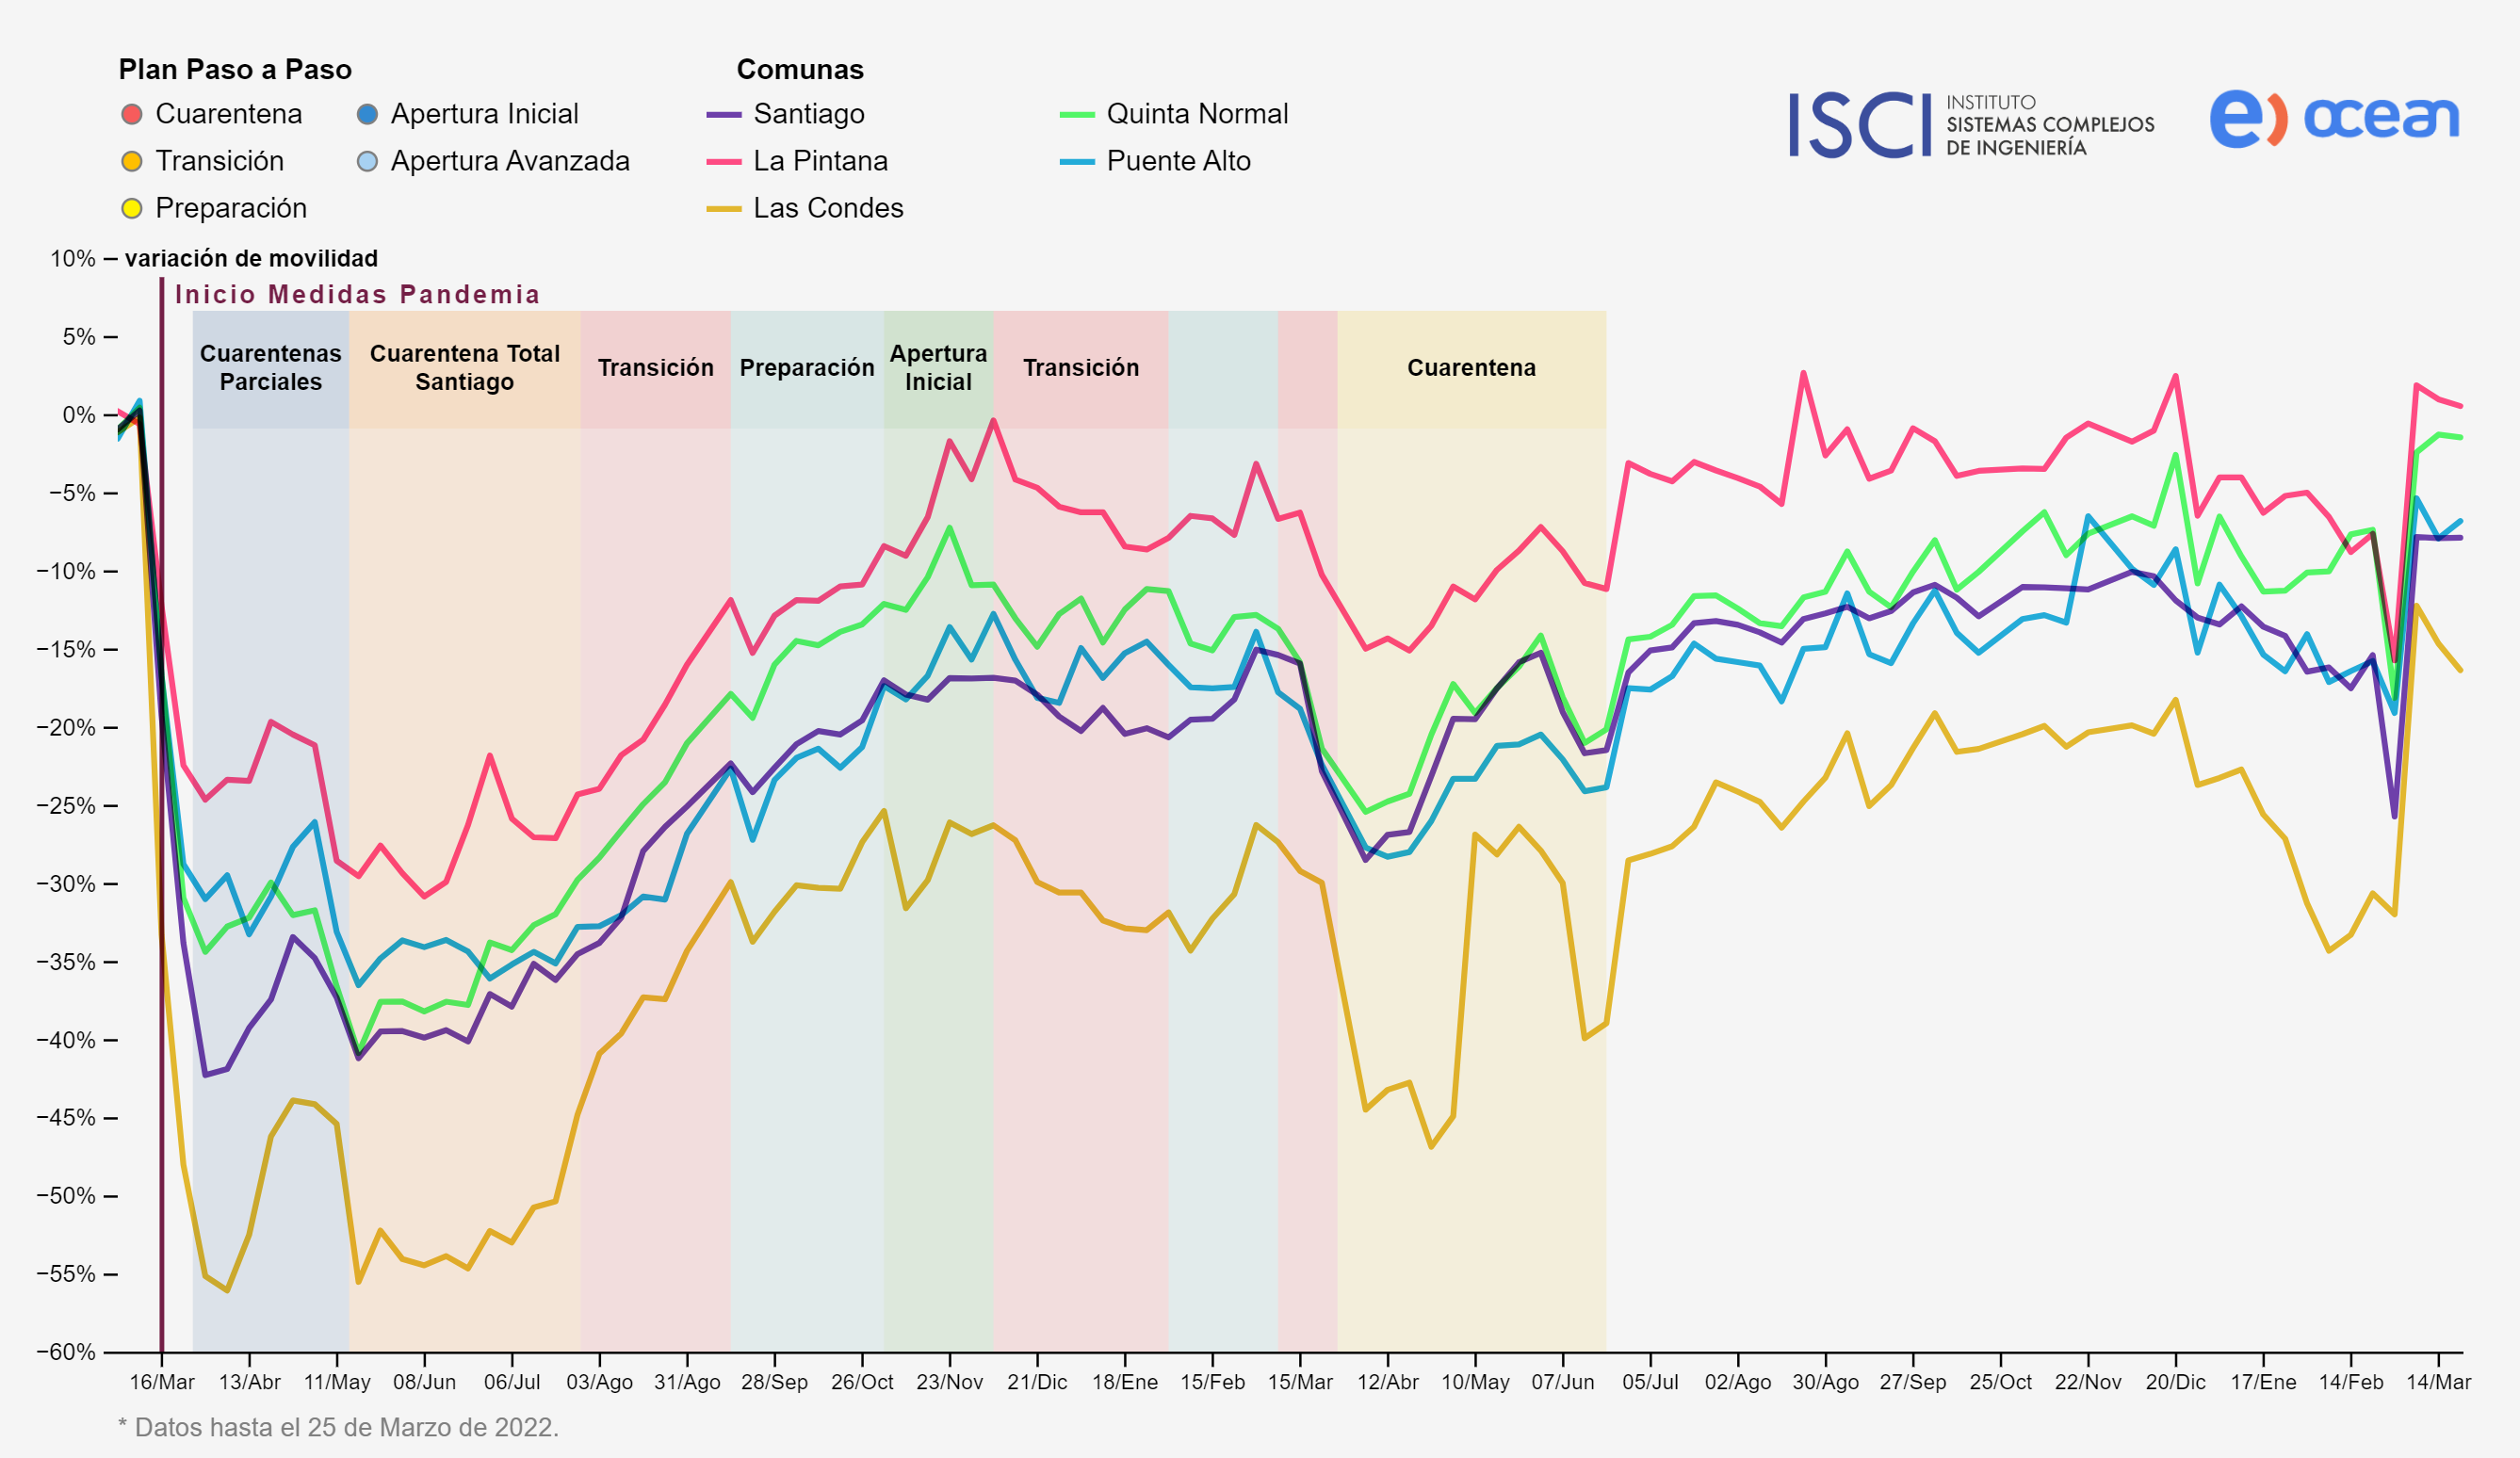
\includegraphics[width=\textwidth]{img/metodologia/datos/movilidad-RM.png}
\caption[Diferencias en la variación de movilidad de cinco comunas de la Región Metropolitana.]{Diferencias en la variación de movilidad de cinco comunas de la Región Metropolitana, desde marzo de 2020 a marzo de 2022. Fuente: ISCI Covid Analytics.}
\label{img:ISCI-movilidad-RM-1}
\end{figure}

La metodología será puesta a prueba estudiando el desarrollo de la pandemia por COVID-19 en la ciudad de Santiago de Chile. Ya desde el comienzo de la pandemia en Santiago, \cite{Olivares2020} hacía notar las dificultades de las clases socioeconómicas más bajas para cumplir las cuarentenas. Esto puede verse claramente en la figura \ref{img:ISCI-movilidad-RM-1}; comunas más acomodadas como Las Condes y Vitacura tienen una reducción de movilidad superior a comunas con menos recursos como La Pintana, a lo largo de toda la pandemia. Varios estudios \cite{Mena2021}\cite{Bennett2021}\cite{Gozzi2021} han notado las significativas diferencias en el impacto de la pandemia en los distintos sectores socioeconómicos de la capital del país, atribuyéndolas, entre otros factores, a la capacidad de cumplimiento de las cuarentenas y las diferencias en el acceso a salud.

Además de lo anterior, el Ministerio de Ciencia, Tecnología, Conocimiento e Innovación de Chile ha hecho disponibles públicamente \cite{MINCIENCIA} varias series de datos epidemiológicos de casos infectados confirmados, hospitalizados, hospitalizados UCI, fallecidos, vacunados, etc. Estos datos poseen diversos niveles de segregación, por comuna, edad o sexo. Todas estas características hacen de la ciudad de Santiago un buen escenario escenario donde implementar el modelo.




\section*{Objetivos}

El objetivo principal del trabajo es estimar el factor sanitario de distintas clases sociales, por medio del \textit{framework} lagrangiano de clases y ambientes de \cite{Bichara2018}. Este objetivo se descompone en dos objetivos específicos. En primer lugar, se necesita definir una metodología que permita estimar el factor sanitario. En segundo lugar, se debe implementar y evaluar la metodología, aplicándola al caso de estudio: la pandemia de COVID-19 en Santiago. 

Definir la metodología requiere plantear el modelo lagrangiano, haciéndole los ajustes necesarios al planteado por \cite{Bichara2018} y considerando las características del COVID-19. Se debe además definir cómo estimar la matriz de tiempos de residencia en base a los datos disponibles. Finalmente, es necesario elegir la variante de filtro de Kalman específica a utilizar en la estimación de parámetros. La implementación requiere de la obtención de datos, el cálculo de la matriz de tiempos de residencia, y la escritura del código para el modelo y el filtro de Kalman.

% Idealmente:
% Este trabajo busca poner a prueba el modelo propuesto en \cite{Bichara2015}, mediante su aplicación al estudio de la evolución de la pandemia de COVID-19 en la ciudad de Santiago de Chile. 
% la idea es que ya no se necesitan las interacciones en cada clase. % Pero a cambio necesito saber en qué ambientes está la gente. 
% De verdad me estoy preguntando qué pasa si solo lo dejo con dos ambientes. Siento que puedo dejarlo con hogar y fuera del hogar. Eso me permitiría meter casi directamente la información de movilidad. Creo que lograría tener movilidad por nivel socioeconómico, en base a la info por comunas. Pero la movilidad por edad creo que está harto más difícil de determinar. 

% Poner a prueba en qué? Bajo qué criterios? El principal criterio es que no necesito conocer cómo interactúa la gente, quiero tener resultados interesantes sin necesariamente saber de qué forma se mezclan todos.

% Cómo puedo evaluar? Comparando la cercanía con los resultados obtenidos con algún otro modelo multiclase?  

%El objetivo general de este trabajo es implementar el \textit{framework} lagrangiano multiclase con dispersión virtual presentado por \cite{Bichara2018}, 

% ... La idea que tengo es... este modelo es lagrangiano, y dice que apaña para evitar tener que calcular las tasas de contacto específicas entre clases, es difícil saber cómo se relaciona la gente... y las opciones que hay son encuestas no necesariamente aplicables. La alternativa presentada es ...

% Una vez que tenemos esa opción...

%Más específicamente, y utilizarlo en la estimación del impacto de las medidas de contención del COVID-19 en la ciudad de Santiago de Chile. 

% Modelos multiclase en Santiagooooo, estoy segura de que hay gente haciendo eso, la fundación ciencia y vida estaba trabajando con un modelo de todas las comunas, haciendo algo parecido a lo que hacía yo pero mucho más complejo. 


% Siempre deben ser verbos terminados en -ar -er -ir 
% Mi objetivo es implementAR el modelo ... qué acciones hay que cumplir 
% \begin{itemize}
% \item Qué compartimientos usar? 
% \item Qué clases elegir? 
% \item Qué ambientes elegir? <-
% \item Cómo formo la matriz de tiempos de residencia, de dónde obtengo los datos? 
% \item Cómo actualizo esa matriz, ya que ha ido cambiando en el tiempo. 
% \item Cómo elijo los parámetros para ajustarlo a los datos existentes de avance de la pandemia? Qué dejo constante? Qué dejo variable? Qué método uso para los constantes? 
% \item Cómo evalúo lo bien que funciona el modelo?
% \end{itemize}

% - Elección del modelo. Esto aún tengo que discutirlo... pero incluye: qué clases usar, que compartimientos usar, cuántos ambientes, etc.
% - Datos disponibles: EOD, datos de movilidad comunal, datos de movilidad de Google por ambiente. Esto para la matriz de 
% - Metodologías dependen de cada objetivo específico 
% - Ajuste del modelo: datos que le voy a dar para ajustar. De qué forma ajusto. 
% - Datos que usaré para verificación, pa cachar qué tan bien funciona la cuestión. 


 

\section*{Metodología}

Para cumplir los objetivos antes expuestos se lleva a cabo la siguiente metodología, la cual se divide en varias etapas. En primer lugar, es necesario explorar las distintas fuentes de datos disponibles, tanto de movilidad y viajes como las series de tiempo epidemiológicas, como cantidad de casos registrados, fallecidos, etc. Esto permite decidir el modelo específico a utilizar, lo que debe considerar las características del COVID-19 para elegir los compartimientos a utilizar (susceptibles, expuestos, infectados, etc), y también los datos disponibles para elegir clases y ambientes.

Una vez decididas las clases y ambientes, es necesario estimar una matriz de tiempos de residencia, que diga cuánto tiempo pasa cada clase en cada lugar. Se desea que esta matriz sea variable en el tiempo, de forma que incorpore cambios en la movilidad causados por las medidas de mitigación, como cuarentenas, teletrabajo, etc.

Todo lo anterior ya permite correr un modelo de la ciudad de Santiago, definiendo factores sanitarios sintéticos y obtener simulaciones. Se busca ahora estimar el factor sanitario a partir de observaciones del modelo. Para esto se utiliza Filtro de Kalman, y es necesario elegir e implementar una de sus muchas variantes (extendido, \textit{unscented}, filtro por ensambles, etc), y elegir cómo usar el filtro para hacer estimación de parámetros (estado aumentado, filtro de Kalman con múltiples modelos, etc).

Posteriormente se estiman los factores sanitarios para cada una de las clases elegidas, ajustando el modelo a los datos reales de la ciudad de Santiago. Para esto es necesario definir qué variables del modelo observar, que datos utilizar como observación y cómo ajustar los parámetros específicos del filtro.

Finalmente, se utiliza la matriz de tiempos de residencia y los factores sanitarios obtenidos para generar varios casos hipotéticos; distintas variaciones en cuarentenas, diferentes niveles de cuidado. Esto entrega varios desarrollos hipotéticos de la pandemia, y se usará para evaluar el modelo.


\section*{Contribuciones y trabajos relacionados}

A continuación se describen las principales contribuciones de este trabajo. En primer lugar, la propuesta de una metodología que permite estudiar las medidas de cuidado de forma independiente a la movilidad. En segundo lugar, la aplicación del \textit{framework} lagrangiano de clases y ambientes presentado por \cite{Bichara2018} a un caso de estudio, lo cual no había sido hecho con anterioridad. Este trabajo guarda, sin embargo, cierta similitud con \cite{Shikhmurzaev}, que plantea un modelo que incorpora patrones de actividad.

En tercer lugar, la implementación en Matlab de la técnica propuesta por \cite{Munizaga2011} de obtención de uso del tiempo partir de los viajes de una Encuesta Origen-Destino. Esta implementación es de código abierto y se encuentra isponible en el repositorio \url{https://github.com/tabitaCatalan/lagrangian-time}. Se utilizan datos de la Encuesta Origen-Destino Santiago 2012.

En cuarto lugar, el desarrollo de una librería, escrita en el lenguaje Julia, para el trabajo con Filtro de Kalman con dinámica y observadores lineales y/o no lineales. Esta se encuentra documentada, es extensible y de código abierto. Está disponible en el repositorio \url{https://github.com/tabitaCatalan/kalman}. Existen librerías similares en el mismo lenguaje como KalmanFilters.jl y Kalman.jl, pero estas no fueron usadas debido a que en la etapa de decidir qué Filtro utilizar, ninguna contaba con todas las opciones que se quería explorar. 

En quinto lugar, el planteamiento de una metodología para el ajuste de los hiperparámetros relacionados a la covarianza del filtro de Kalman, al estimar parámetros de un modelo epidemiológico. Este era un vacío en trabajos como \cite{Hasan2020} y \cite{Sameni2020}, donde se limitan a elegir un valor fijo para el caso particular que trabajan, sin ofrecer una justificación.

Finalmente, la aplicación del modelo al desarrollo de la pandemia de COVID-19 en la ciudad de Santiago de Chile, lo que permite una estimación de la vulnerabilidad/factor sanitario, de forma independiente a la movilidad. Modelos anteriores de Santiago como \cite{Gozzi2021} solo consideran movilidad.


\section*{Estructura de la tesis}
El resto de esta tesis está organizado como sigue. El capítulo \ref{chap:marco} establece las bases para entender el trabajo realizado. Se presentan varios conceptos relevantes de modelos epidemiológicos y de la teoría de filtro de Kalman. Se exponen también los antecedentes del caso de estudio; la enfermedad COVID-19 y su desarrollo en la ciudad de Santiago de Chile.

El capítulo \ref{chap:metod} justifica y detalla los procedimientos seguidos; cómo se usó el framework de \cite{Bichara2018}, los datos utilizados, los supuestos y simplificaciones hechas, el modelo final utilizado y las técnicas específicas implementadas.

El capítulo \ref{chap:results} presenta los principales resultados obtenidos; la matriz de tiempos de residencia, el caso sintético utilizado para ajustar los parámetros del filtro de Kalman y las estimaciones para el factor sanitario obtenidas utilizando datos reales. Se muestran también los diferentes escenarios hipotéticos generados a partir de esas estimaciones.

El capítulo \ref{chap:discus} discute los resultados obtenidos para el caso de estudio, sus implicaciones y limitaciones. Comenta además el  \textit{framework} lagrangiano planteado en \cite{Bichara2018}, sus ventajas y dificultades a la hora de implementarlo. Se plantean posibles extensiones y trabajo futuro.



\end{intro}
%%%%% ESTABLECER QUE EL NIVEL SOCIOECONOMICO NO QUEREMOS DEJARLO FUERA

%%%%%%%%%%%%%%%%%%%%%%%%%%%%%%%%%%%%%%%%%%%%%%%
% Indice 
%%%%%%%%%%%%%%%%%%%%%%%%%%%%%%%%%%%%%%%%%%%%%%%
% Enfermedades contagiosas y la amenaza que suponen. % Esto habla de la importancia del tema.
% Modelos epidemiológicos en general 
%\include{1-1-modelosepi}
% El modelo que nos interesa. También decir por qué es interesante y de qué limitaciones intenta hacerse cargo.
%\include{1-2-virtualdispersal}
% Con todo eso de arriba estoy estableciendo y delimitando mi territorio. 

% Ahora establezco mi nicho 
% El modelo no ha sido utilizado con datos reales ... blah blah 




\chapter{Marco teórico}

% Para pasar a la parte más matemática, debería comenzar con sistemas lineales y no lineales, que es lo más general. Esto me permite enmarcar filtro de kalman y sistema epidemiológicos dentro de una misma cosa.
% Luego puedo pasar a modelos epidemiológicos, para describir el Rt 
% O bien puedo pasar al filtro de Kalman. 

% Discutir idea de estado, modelo, etc. 
% El objetivo de este apartado es dar las bases teóricas que serán necesarias para comprender la metodología seguida. 
% También aquí debería incluirse una revisión bibliográfica. 

En este apartado se presentarán las bases teóricas que sustentan el trabajo realizado. A lo largo de este trabajo se dan por sentadas varias nociones de sistemas lineales y no lineales, ya sea continuos o discretos. Estas se encuentran en el Anexo \ref{sec:lineal}.

Este capítulo se organiza como sigue; en primer lugar, en la sección \ref{sec:epi-model}, se presentan los modelos epidemiológicos compartimentales deterministas, y se explican dos enfoques que permiten tratar con poblaciones heterogeneas: lagrangiano y euleriano. 

En segundo lugar, la sección \ref{modelo-clases-vs-ambientes} presenta el modelo lagrangiano propuesto en \cite{Bichara2015}, que se usará en este trabajo. En tercer lugar, la sección \ref{sec:R0} presenta la técnica de la matriz de próxima generación, esencial en la estimación del número reproductivo básico \(\mathcal{R}_0\).
% Estructura del apartado 

La sección \ref{sec:kalman} está dedicada a la teoría del Filtro de Kalman, una técnica que permite la estimación de estados en sistemas lineales y que ha sido ampliamente extendida y utilizada, contando con aplicaciones en diversos ámbitos de ingeniería y ciencias como climatología, control de vehículos autónomos, etc. Se presentará la teoría básica del filtro y las principales extensiones que se utilizan durante el trabajo.

Contando ya con las bases teóricas, la sección \ref{sec:antecedentes} presenta los antecedentes relevantes al caso de estudio a tratar; el brote de Covid-19 en la ciudad de Santiago de Chile. Se describen características particulares de esta enfermedad y cómo influyen en el modelamiento. Se presentan características de la ciudad de Santiago que han influido el desarrollo de la pandemia y las medidas tomadas para ralentizar su avance.


%%%%%%%%%%%%%%%%%%%%%%%%%%%%%%%%%%%%%%%%%%%%
% Índice 
%%%%%%%%%%%%%%%%%%%%%%%%%%%%%%%%%%%%%%%%%%%%
% Explicación de la idea de estados, debería ser lo primero porque se va a usar mucho. 

% Sistemas lineales y no lineales, discretización, conceptos que se necesitan como base para entender todo el resto 
% \include{2-1sistemaslineales} % ahora en el anexo

% 


\section{Modelos epidemiológicos}\label{sec:epi-model}

Se presentan ahora los modelos epidemiológicos compartimentales deterministas. Primero, \ref{subsec:sir-seir} explica brevemente los modelos SIR y SEIR. A continuación, \ref{subsec:euler-lag} explica los enfoques lagrangiano y euleriano, que permiten tratar con poblaciones heterogéneas. Finalmente, \ref{modelo-clases-vs-ambientes} presenta el modelo lagrangiano propuesto en \cite{Bichara2018} que se usará en este trabajo.

\subsection{Modelos compartimentales SIR y SEIR}\label{subsec:sir-seir}

Los modelos compartimentales son ampliamente utilizados a la hora de modelar una enfermedad contagiosa. La idea tras ellos es simple: separar a la población en grupos o compartimientos de acuerdo al grado de avance de la enfermedad, y asignar reglas para pasar de un compartimiento a otro.

Un modelo muy sencillo es el \textbf{SIR}, que separa a la población en \textbf{S}usceptibles, \textbf{I}nfectados y \textbf{R}emovidos. En este trabajo se trata este modelo de manera determinista, viéndolo como el sistema de ecuaciones diferenciales ordinarias \ref{eq:sir}, pero también es posible tratarlo de manera estocástica \cite{Daley1984}.

\begin{equation}
\label{eq:sir}
\begin{aligned}
S'(t) &=  -\alpha \frac{S(t)I(t)}{N} \\
I'(t) &= \alpha \frac{S(t)I(t)}{N}- \gamma_I I(t) \\
R'(t) &= \gamma_I I(t).
\end{aligned}
\end{equation}

Los susceptibles son el grupo de la población que puede ser contagiado con la enfermedad. La enfermedad solo es propagada por los individuos infectados. Cuando un susceptible se infecta, inmediatamente comienza a contagiar a otros. Tras un tiempo los infectados dejan de contagiar y son removidos. Esto puede deberse a una recuperación de la enfermedad con inmunidad completa (no pueden volver a contagiarse), al aislamiento del contagiado o bien a su muerte debido a la enfermedad. El diagrama de flujo para pasar de un compartimiento a otro puede verse en la figura \ref{fig:sir}.

En este modelo, el total de la población dado por \(N = S + I + R\) permanece constante a lo largo del tiempo. Este modelo supone que un individuo hace en promedio \(\alpha\) contactos  ``efectivos'' o ``suficientes'' para contagiar la enfermedad por unidad de tiempo. Esto, en conjunto con la probabilidad \(S/N\) de que el individuo contactado sea susceptible, deja una cantidad de \(\alpha S I / N\) nuevos contagios por unidad de tiempo. Suponer una tasa de recuperación de la forma \(\gamma_I I\), con \(\gamma_I\) un valor positivo, implica un periodo de infección con distribución exponencial y media \(1/\gamma_I\) (más detalles en \cite{Brauer2019}).




% \ctikzfig{sir}
\begin{figure}[!h]
\centering
\begin{tikzpicture}
	\begin{pgfonlayer}{nodelayer}
		\node [style=black-edge] (0) at (-9, 0) {$S$};
		\node [style=black-edge] (4) at (-1, 0) {$R$};
		\node [style=black-edge] (5) at (-5, 0) {$I$};
		\node [style=none] (6) at (-7, 0.5) {$\alpha I/N$};
		\node [style=none] (7) at (-3, 0.5) {$\gamma_I$};
	\end{pgfonlayer}
	\begin{pgfonlayer}{edgelayer}
		\draw [style=arrow] (0) to (5);
		\draw [style=arrow, in=180, out=0] (5) to (4);
	\end{pgfonlayer}
\end{tikzpicture}

\caption{Diagrama de flujo del modelo SIR dado por las ecuaciones \ref{eq:sir}.} \label{fig:sir}
\end{figure}



Es posible complejizar este modelo añadiendo compartimientos extras. El compartimiento de \textbf{E}xpuestos permite pasar por un periodo de incubación o latencia, de \(1/\gamma_E\) en promedio, antes de comenzar a contagiar la enfermedad, como se ve en las ecuaciones \ref{eq:seir}. Esto da lugar al modelo \textbf{SEIR}, cuyo diagrama puede verse en la figura \ref{fig:seir}. Es posible agregar otro compartimientos como hospitalizados, fallecidos, etc. Desde luego, los compartimientos del modelo dependen de la enfermedad a modelar.


\begin{equation}
\label{eq:seir}
\begin{aligned}
S' &=  -\alpha \frac{SI}{N} \\
E' &= \alpha \frac{SI}{N} - \gamma_E E \\
I' &= \gamma_E E - \gamma_I I \\
R' &= \gamma_I I.
\end{aligned}
\end{equation}


% \ctikzfig{sir}
\begin{figure}[!h]
\centering
\begin{tikzpicture}
	\begin{pgfonlayer}{nodelayer}
		\node [style=black-edge] (0) at (-9, 0) {$S$};
		\node [style=black-edge] (4) at (-1, 0) {$I$};
		\node [style=black-edge] (5) at (-5, 0) {$E$};
		\node [style=none] (6) at (-7, 0.5) {$\alpha I/N$};
		\node [style=none] (7) at (-3, 0.5) {$\gamma_E$};
		\node [style=black-edge] (8) at (3, 0) {$R$};
		\node [style=none] (9) at (1, 0.5) {$\gamma_I$};
	\end{pgfonlayer}
	\begin{pgfonlayer}{edgelayer}
		\draw [style=arrow] (0) to (5);
		\draw [style=arrow, in=180, out=0] (5) to (4);
		\draw [style=arrow] (4) to (8);
	\end{pgfonlayer}
\end{tikzpicture}
\caption{Diagrama de flujo del modelo SEIR dado por las ecuaciones \ref{eq:seir}.} \label{fig:seir}
\end{figure}



\subsection{Enfoques euleriano y lagrangiano}\label{subsec:euler-lag}

Los modelos dados por las ecuaciones \ref{eq:sir} y \ref{eq:seir} suponen que la población se mezcla perfectamente, de forma que las interacciones entre individuos son homogéneas. Una forma de incluir heterogeneidad es separar a la población en grupos, en un modelo multiclase. Esto permite considerar las distintas capacidades de enfrentar y sobrevivir a la enfermedad de cada grupo, así como las diferencias en comportamiento.

La edad es un factor a considerar en varias enfermedades; niños menores de 5 años son especialmente vulnerables a enfermedades como la malaria o la tuberculosis. Adultos mayores tienen mayor probabilidad de experimentar síntomas graves al contraer influenza. En las enfermedades de transmisión sexual, las parejas tienen edades similares en muchos casos. Para más detalles de cómo considerar la edad dentro del modelamiento epidemiológico puede verse el capítulo 13 de \cite{Brauer2019}.

La ubicación espacial es otro factor a tener en cuenta; en una sociedad interconectada las enfermedades se propagan rápidamente entre un lugar y otro, y cambios en los patrones de movimiento alteran la transmisión de una enfermedad. Este tema es tratado brevemente en el capítulo 14 de \cite{Brauer2019}.

El objetivo de esta subsección es presentar dos enfoques distintivos que se observan al utilizar modelos con mezcla espacial heterogénea; euleriano y lagrangiano. Los nombres derivan de cierta similitud entre estos enfoques y las especificaciones euleriana y lagrangiana del movimiento de fluidos; en el enfoque lagrangiano, es posible ``seguir la trayectoria'' de las personas/partículas, mientras que en el euleriano, el enfoque está en las regiones y en los flujos de personas/partículas que entran o salen de ahí. Estas definiciones son bastante generales y no son excluyentes entre sí \cite{Cosner2009}.

Se supone una situación con \(n\) regiones, donde la personas puede moverse de una región a otra. Por simplicidad se supone además que infección no altera los patrones de movimiento de la población.\\


%\noindent \textbf{Enfoque euleriano}
\subsubsection*{Enfoque euleriano}

El enfoque euleriano podría describirse como ``migratorio''; las personas no pertenecen a ninguna región, sino que se mueven entre ellas. El movimiento de la población entre dos regiones cualesquiera es conocido.

Se presenta ahora un ejemplo más específico, tomado de una simplificación del modelo euleriano de \cite{Hsieh2007}. Se supone conocida una matriz \(C = (c_{ij})_{i, j = 1\dots n}\) de tasas de migración entre regiones.  \(c_{ij} \geq 0\) corresponde al número de personas por unidad de tiempo que sale desde la región \(i\) hacia la región \(j\). Por definición \(c_{ii} = 0\). 


Similar a \cite{Cosner2009}, si \(N_i(t)\) corresponde a la población presente en la región \(i\) a tiempo \(t\), entonces se puede formar un modelo migratorio considerando las personas que salen y las que entran, con las ecuaciones \ref{eq:migration}.

\begin{equation}\label{eq:migration}
N_i' = \sum_{j = 1}^n c_{ji} N_j - \sum_{j = 1}^n c_{ij} N_i.
\end{equation}

Luego, es posible considerar la propagación de la enfermedad dentro de cada región. Si \(S_{i}(t), I_i(t)\) corresponden al número de susceptibles e infectados en la región \(i\) a tiempo \(t\), y \(\alpha_{i}\) es el número promedio de contactos efectivos que hace un individuo en la región \(i\). La dinámica de los susceptibles en este ejemplo puede verse en la ecuación \ref{eq:migration-transmis}.

\begin{equation}\label{eq:migration-transmis}
S'_i = - \alpha_i\frac{S_iI_i}{N_i}.
\end{equation}

%\noindent \textbf{Enfoque lagrangiano}
\subsubsection*{Enfoque lagrangiano}

Otra forma de modelar esta situación es enfocarse en las personas; cada una habita en cierta región, aunque puede visitar otras regiones. Esto permite calcular el número de infectados que residen (no están solo de visita) en cada región. Los habitantes de una región usualmente comparten parámetros epidemiológicos (tasa de exposición, recuperación, etc). 

Los nuevos contagios se calculan a partir del número de infectados y susceptibles presentes en la región, comparado al total de personas en cada región, que pueden ser visitantes de otras regiones, o habitantes de esa región.

Un ejemplo de modelo lagrangiano se encuentra en \cite{Ruan2006}. Este define \(S_{ij}(t), I_{ij}(t), R_{ij}(t)\) como los suceptibles, infectados y recuperados de la clase \(i\) que se encuentran en la clase \(j\) a tiempo \(t\).  Esto permite calcular, definiendo \(N_{ij} = S_{ij} + I_{ij} + R_{ij}\), el total de residentes de la región \(i\) como \(N^r_i := \sum_{j = 1}^n N_{ij}\) y el total de personas presentes en la región \(i\) como \(N^p_i := \sum_{j = 1}^n N_{ji}\). La tasa de infección de la población de la región \(i\) debido a los contagios producidos en la región \(k\) se calcula simplemente como la suma de todos los contactos efectivos entre susceptibles de la clase \(i\) con algún infectado de cualquier clase, como se ve en la ecuación \ref{eq:lagran-trans}. \(\alpha_{ikj}\) corresponde a la cantidad de contactos efectivos entre la clase \(i\) y la clase \(j\) que ocurren en la región \(k\).

\begin{equation}\label{eq:lagran-trans}
S'_{ik} = -\sum_{j = 1}^n \alpha_{ikj} \frac{S_{ik}I_{jk}}{N^p_j}.
\end{equation}

Este modelo, guardando similitud con el modelo euleriano expuesto antes, supone que los residentes susceptibles de la región \(i\) viajan a otras regiones a una tasa constante \(\sigma_i\). Desde la región \(i\) van a la región \(j\) con probabilidad \(\nu_{ij}\), y vuelven a su región con tasa \(\rho_{ij}\). Esta, sin embargo, no es la única forma de trabajar con la movilidad de la población. Los artículos \cite{Cosner2009} y \cite{Bichara2015} utilizan matrices \(P = (p_{ij})_{i, j = 1 \dots n}\) de tiempos de residencia, donde \(p_{ij}\) corresponde a la fracción de su tiempo que los residentes de la clase \(i\) pasan en la región \(j\). Desde luego se cumple \(\sum_{j = 1}^n p_{ij} = 1\) para cada \(i\). Esta forma de abordar la movilidad será la más interesante para este trabajo, y se verá en más detalle en la siguiente sección.






\subsection{Modelo multiclase con dispersión virtual}\label{modelo-clases-vs-ambientes}

Si bien separar a la población en distintos grupos permite incorporar heterogeneidad en las interacciones, estos modelos añaden dificultades extra, puesto que ahora es necesario conocer de qué manera interactúan los distintos grupos. La primera dificultad reside en la noción de contacto efectivo. Si bien esta es clara en el contexto de enfermedades de transmisión sexual o enfermedades transmitidas por vectores (como la malaria y el dengue, que son transmitidas por mosquitos), el concepto es mucho más vago al referirnos a enfermedades transmitidas por contacto estrecho o por microgotas al toser, estornudar o hablar.

Otra dificultad está en la necesidad de conocer en gran detalles las interacciones entre grupos. En la sección anterior, el modelo euleriano presentado requería una matriz \(C = (c_{ij})_{i,j = 1 \dots n} \) con las tasas de migración entre cualquier par de regiones. El modelo lagrangiano, similarmente, requería las probabilidades \(\nu_{ij}\) de pasar de una región a otra, para cualquier par de regiones. Más aún, necesitaba de una matriz \(\alpha_{ikj}\) que detallara quién estaba en contacto con quién y dónde.

Este tipo de matrices de contacto es conocida como WAIFW (\textit{Who Acquires Infection From Whom} o  ¿Quién adquiere la infección de quién?) \cite{Anderson1992}. Este tipo de matrices suelen aproximarse por matrices de ``mezcla social'' o \textit{social mixing}; varios ejemplos para enfermedades transmitidas por contactos estrechos son \cite{Mossong2008}\cite{Wallinga2006}\cite{Edmunds2006}.

\cite{Bichara2015} sugiere una solución alternativa; utilizar un modelo lagrangiano con tiempos de residencia. De esta forma, el tiempo pasado en cada región y su riesgo sirve como \textit{proxy} de la probabilidad de contagios. \cite{Bichara2015} propone dos variantes de esta idea; en la primera, cada clase pertenece a una región pero pasa un tiempo en las otras regiones. Esta forma de abordar el problema es utilizada también por \cite{Cosner2009}. En la segunda variante, las clases interactúan en ambientes como hospitales, centros comerciales, escuelas, transporte público, lugares de trabajo, etc. Esto permite combinar clases y dispersión espacial en un mismo modelo. Esta variante es extendida posteriormente en \cite{Bichara2018} y es la que se usa en este trabajo.

%\textbf{euleriano} vs \textbf{lagrangeano} [Esto no he logrado entenderlo bien, las explicaciones son muy cortas].

% El primer modelo propuesto por \cite{Bichara2015} considera \(n\) clases, cada una de las cuales reside en una región (\textit{patch}). \(N_i(t), i = 1, \dots, n\) denota a la cantidad de personas que residen en la región \(i\) y \(p_{ij} \in [0,1]\) representa la fracción de tiempo que la clase \(i\) pasa en la región \(j\). En este trabajo, sin embargo, usaremos el modelo alternativo propuesto en el mismo artículo y desarrollado más ampliamente en \cite{Bichara2018}.
Se separa a la población en \(n\) clases, las cuales interactúan en \(m\) ambientes o áreas de riesgo. \(N_i(t), i = 1, \dots, n\) corresponde a la población de la clase \(i\). Suponemos que la población de la clase \(i\) pasa una proporción \(p_{ij} \in [0,1]\) de su tiempo en el ambiente \(j\), con \(\sum_{j = 1}^{m} p_{ij} = 1\) para cada \(i\). Para casos extremos, por ejemplo, podría darse que \(p_{ij} = 0\), es decir, la clase \(i\) no gasta nada de su tiempo en el ambiente \(j\), mientras que \(p_{ij} = 1\) significa que la clase \(i\) pasa todo su tiempo en el ambiente \(j\). 

Para ejemplificar se usan compartimientos SIR, sin embargo, esta metodología puede extenderse a otros compartimientos. Las ecuaciones en este caso están dadas por \ref{eq:virtual-disp}, donde \(\lambda_i\) está dado por \ref{eq:lambda}. Los términos \(b_i\) y \(d_i\) representan las tasas de natalidad y mortalidad de la clase \(i\) respectivamente.

\begin{equation}\label{eq:virtual-disp}
\begin{aligned}
%S_i(t)' &= -S_i(t) {\color{Red} \lambda_i(\vec{x}, t) } \\
S_i(t)' &=  b_i - d_i S_i - {\lambda_i(\vec{x}, t) } \\
I_i(t)' &= {\lambda_i(\vec{x}, t) } - \gamma_i I_i(t) - d_i I_i\\
R_i(t)' &= \gamma_i I_i(t)\\ 
\end{aligned}
\end{equation}

\begin{equation}\label{eq:lambda}
\lambda_i(\vec{x}, P) = \sum_{j=1}^m \beta_{j}p_{ij}S_i(t)\frac{\sum_{k=1}^{n} p_{kj} I_k}{\sum_{k=1}^{n} p_{kj}N_k}
\end{equation}

El valor \(\beta_j\) es una medida de riesgo propio del ambiente \(j\)-ésimo y depende de las condiciones ambientales y sanitarias. Representa la idea de que no es lo mismo pasar el tiempo en un parque que en el transporte público o en un bar.  la distancia que mantienen las personas ahí, la ventilación, entre otras.

Puesto que \(p_{ij}\) es la proporción del tiempo que la clase \(i\) reside en el ambiente \(j\), entonces la cantidad de personas en promedio de la clase \(i\) en el ambiente \(j\), en algún momento de tiempo \(t\), está dada por \(N_i(t) p_{ij} = S_i(t) p_{ij} + I_i(t) p_{ij} + R_i(t) p_{ij}\). La población total en el ambiente \(j\) es \(\sum_{k = 1}^m N_k p_{ij}\), de la cual \(\sum_{k = 1}^m I_k p_{ij}\) están infectados. De esta forma, el número de infectados de la clase \(i\) en el ambiente \(j\) por unidad de tiempo está dado por la ecuación \ref{eq:infectados-explicado}.

\begin{equation}\label{eq:infectados-explicado}
\underbrace{b_j}_{\text{riesgo}} \cdot \underbrace{S_i p_{ij}}_{\substack{\text{susceptibles}\\\text{de la clase } i\\ \, \text{en el ambiente } j}} \cdot \underbrace{\frac{\sum_{k = 1}^m I_k p_{ij}}{\sum_{k = 1}^m N_k p_{ij}}}_{\substack{\text{proporción}\\\text{de infectados}\\\text{en el ambiente }j}}
\end{equation}


El modelo presentado supone que la etapa de la enfermedad no afecta el comportamiento de la población. Una forma más completa de modelarlo es seguir a \cite{Bichara2018} y utilizar distintas matrices de tiempos de residencia para cada compartimiente, representando la idea de que los infectados se queden en su casa guardando cuarentena, por ejemplo.
% estado del arte. Uso en Covid 
%El modelo original ha sido usado por Baltazar Espinoza (\textit{Mobility restrictions for the control of epidemics: When do they work?}) para mostrar la ineficacia de los cordones sanitarios para reducir la cantidad total de infectados, si se usan, por ejemplo, para aislar una población de una región de bajo riesgo (una baja densidad poblacional por ejemplo) y buen acceso a salud de una de alto riesgo y acceso sanitario deficiente. 






% Modelos epidemiológicos como un caso particular de sistemas no lineales. 
\section{Número reproductivo básico y efectivo}\label{sec:R0}

%Se sigue la explicación dada por \cite{Brauer2019}, que está basada en [Buscar autores].

El número reproductivo básico \(\mathcal{R}_0\) se define como el número esperado de casos de una enfermedad producidos por un individuo `típico' en una población completamente susceptible [Tal vez cita, es traducción directa]. Solo se consideran las infecciones secundarias (las producidas por ese individuo, y no las producidas por otros que fueron infectados por él). Para epidemias donde se pueden ignorar los efectos demográficos y donde tras enfermarse los individuos tienen inmunidad completa, la línea \(\mathcal{R}_0=1\) es la línea divisoria entre una infección que desaparece (\(\mathcal{R}_0<1\)) y una que se transforma en una epidemia (\(\mathcal{R}_0>1\)).

Una forma bastante general para calcularlo en modelos de ecuaciones diferenciales es usar la \textit{next generarion matrix}. La idea es la siguiente: separar los compartimientos en dos tipos: enfermo y sano. Los enfermos no necesariamente son contagiosos. Si hay \(n\) compartimientos de tipo enfermo, \(m\) de tipo sano y \(x \in \mathbb{R}^n, y \in \mathbb{R}^m\) son subpoblaciones de cada uno de esos compartimientos. Denotaremos \(\mathcal{F}_i\) al flujo de entrada al compartimiento \(i\)-ésimo debido a infecciones secundarias y \(\mathcal{V}_i\) al flujo de salida del compartimiento \(i\)-ésimo debido a progresión de la enfermedad, recuperación o muerte. Esto permite escribir 
\begin{equation}
\label{model-flows}
\begin{aligned}
x_i' &= \mathcal{F}_i(x,y) - \mathcal{V}_i(x,y) & i = 1, \dots, n \\ 
y_j' &= g_j(x,y) & j = 1, \dots, m
\end{aligned}
\end{equation}

Se consideran los siguientes supuestos 
\begin{itemize}
\item \(\mathcal{F}(0, y) = 0\) y \(\mathcal{V}(0, y) = 0\) para \(y \geq 0\). Esto dice que todas las nuevas infecciones son secundarias, provienen de alguien infectado dentro del sistema; no hay inmigración de individuos infectados hacia los compartimientos de enfermedad.
\item El sistema libre de enfermedad \(y' = g(0,y) \) tiene un único equilibrio que es asintóticamente estable, ie. todas las soluciones con condiciones iniciales \((0,y)\) se aproximan a un punto \((0, y_0)\) a medida que \(t \to \infty\). Esto asegura que el equilibrio libre de enfermedad es un equilibrio del sistema.
\item \(\mathcal{F}_i(x,y) \geq 0\) para \(x,y\) no negativos e \(i = 1, \dots, n\).
\item \(\mathcal{V}_i(x,y) \leq 0\) si \(x_i = 0\), \(i = 1, \dots, n\).
\item \(\sum_{i=1}^n\mathcal{V}_i(x,y) \geq 0\) si \(x,y\) son no-negativos.
\end{itemize}

Supongamos que introducimos una persona infectada al sistema libre de enfermedad. Si linealizamos en torno al punto de equilibrio libre de enfermedad \(0, y_0\) notamos que 
\[
\frac{\partial \mathcal{F}_i}{\partial y_j} (0,y_0) = \frac{\partial \mathcal{V}_i}{\partial y_j} (0,y_0) = 0
\]

Esto implica que las ecuaciones para los compartimientos de enfermedad está desacopladas del resto, por lo que se pueden escribir como 
\[
x' = (F-V)x
\]
Donde 
\[
F = \frac{\partial \mathcal{F}_i}{\partial x_j}(0, y_0) \quad
V = \frac{\partial \mathcal{V}_i}{\partial x_j}(0, y_0) 
\]

Llamamos a la matriz \(FV^{-1}\) la \textit{matrix de próxima generación} o \textit{next generation matrix}. Su radio espectral \(\rho\), es decir, el valor propio con mayor módulo, corresponde a \(\mathcal{R}_0 = \rho(FV^{-1})\).

\begin{teo}
El equilibrio libre de enfermedad de \ref{model-flows} es localmente asintóticamente estable si \(\mathcal{R}_0 < 1\) pero inestable si \(\mathcal{R}_0 > 1\).
\end{teo}





% Filtro de Kalman, una teoría específica de sistemas lineales que vamos a utilizar 
\section{Filtro de Kalman}\label{sec:kalman}

% Una vez que se tiene el modelo, si se quiere aplicar a un contexto específico, es necesario incorporar los datos para ajustar los parámetros. Dos técnicas conocidas y ampliamente utilizadas para esto son, por una parte, resolver el problema de minimización de una función de costo dada por la diferencia entre los valores dados por el modelo y las observaciones, sobre los posibles parámetros. Por otra parte, es posible seguir un enfoque bayesiano, asignando densidades a priori a cada parámetro y luego usando los datos para actualizar esas densidades mediante el método de Monte Carlo. Una posibilidad menos explorada es la asimilación de datos usando el Filtro de Kalman.

Filtro de Kalman es un método ampliamente utilizado en diversas aplicaciones de ingeniería como navegación, control de vehículos, procesamiento de señales, etc \cite{Auger2013}. Se tiene un sistema cuya evolución está dada por ciertas ecuaciones. El estado del sistema es desconocido pero se cuenta con observaciones ruidosas de este. El objetivo es estimar el estado a partir de estas observaciones; por ejemplo, estimar la posición de un vehículo cuando solo se conoce su velocidad.

Para un instante \(k\)-ésimo, hay tres formas importantes de estimación del estado \(x_k\) del sistema. El suavizado (\emph{smoothing}) intenta obtener la mejor estimación posible de \(x_k\) usando la información, es decir las observaciones, disponibles hasta un instante posterior \(k+m\). El filtraje solo dispone de información hasta la iteración \(k\)-ésima, y la predicción tiene información hasta una iteración anterior \(k-m\). Debido a la cantidad de información que conoce, el suavizado desde luego debería dar el mejor resultado de los tres, seguido por el filtraje y finalmente la predicción. 

Si bien en su versión original el filtro de Kalman estaba enfocado en un problema lineal gaussiano \cite{Kalman1960}, han surgido diversas variantes para generalizarlo a otros problemas. Algunas de las más conocidas son el Filtro de Kalman Extendido (EKF) o el Filtro ``sin olor'' \textit{Unscented} (UKF) \cite{Cai2006}, que permiten trabajar con sistemas no lineales, el Filtro de Kalman por Ensambles (EnKF) \cite{Katzfuss2016}, que es menos costoso computacionalmente y que puede usarse en problemas con gran cantidad de estados, o el Filtro H\(^\infty\) que es más robusto ante incertezas en el modelo. Varios de estos filtros tienen versiones continuas y discretas \cite{Kulikov2014}.

Esta sección está fuertemente basada en \cite{Anderson2005} y \cite{Simon2006}, y se estructura como sigue: en la subsección \ref{filtro-lineal} comenzaremos estudiando en detalle el filtro de Kalman para el caso más sencillo, en que el sistema es lineal y gaussiano. A continuación, la subsección \ref{filtro-extendido} presenta el Filtro de Kalman Extendido, una variante que permite trabajar con sistemas no lineales, y que es la que usaremos en el trabajo.

Finalmente se exponen algunas técnicas que serán de utilidad. La subsección \ref{estimacion-de-parametros} muestra una forma de estimar parámetros desconocidos de la dinámica del sistema. La subsección \ref{casiperfect} muestra una forma de incorporar restricciones a las estimaciones, y la subsección \ref{smoother} se aparta del filtraje para presentar una forma de suavizado cuando son conocidas todas las observaciones para un intervalo de tiempo.

\subsection{Filtro de Kalman lineal discreto}\label{filtro-lineal}

Para comenzar a explicar el filtro de Kalman, se decide utilizar un caso sencillo. Se tiene un sistema como el de la ecuación \ref{eq:kalman-lineal-discreto}, donde \(x_k \in \mathbb{R}^{n}\) y \(F_k, G_k \in \mathbb{R}^{n \times n}\) y \(w_k \sim \mathcal{N}(0,Q_k)\) es un vector aleatorio que representa un ruido gaussiano en la dinámica del sistema. 

\begin{equation}\label{eq:kalman-lineal-discreto}
x_{k+1} = F_k x_k + G_k w_k
\end{equation}

Los estados \(x_k\) del sistema son desconocidos, y solo es posible conocer observaciones \(y_k\) de ellos, dadas por la ecuación \ref{eq:kalman-lineal-discreto-obs}, donde \(y_k \in \mathbb{R}^{m}, H_k \in \mathbb{R}^{m \times n}\) y \( v_k \sim \mathcal{N}(0, R_k)\) representa un ruido gaussiano en las observaciones.

\begin{equation}\label{eq:kalman-lineal-discreto-obs}
y_k = H_k x_k  + v_k
\end{equation}


Para una condición inicial gaussiana \(x_0 \sim \mathcal{N}(\hat{x}_0, P_0)\), la linealidad del sistema y el hecho de que el ruido es gaussiano, implica que cada uno de los \(x_k\) serán también gaussianos. Se busca estimar \(x_k\) a partir de las observaciones \(y_k\). Más específicamente, en términos bayesianos, se busca la distribución \textit{a posteriori} de \(x_k\) dado un conjunto de observaciones \(y_{1:l} := \{y_1, \dots, y_l\}\). Denotaremos a esta distribución \(x_{k,l}:= x_k | y_{1:l}\).

Existen tres formas de estimación, que dependen del valor de \(l\); en primer lugar, si \(l < k\), se está intentando estimar \(x_k\) con información hasta un instante \(l\) anterior a \(k\). A esta forma se le llama predicción o \textit{forecasting}. En segundo lugar, si \(l>k\), entonces se está estimando \(x_k\) con información hasta un instante \(l\) posterior a \(k\). Se llamará a esto suavizado o \textit{smoothing}. Finalmente, si \(l = k\) se llamará filtraje o \textit{filtering}. Es esta última forma la que nos presenta mayor interés y que facilita la explicación, por lo que es la forma que será utilizada.

Se sigue el siguiente procedimiento. Se comienza suponiendo que la distribución a posteriori de \(x_{k-1}\) con observaciones hasta el instante \(k-1\) es conocida, \(x_{k-1, k-1} \sim \mathcal{N}(\hat{x}_{k-1, k-1}, P_{k-1, k-1})\); se busca la distribución \(x_{k, k}\). Esto se logra mediante una iteración del filtro de Kalman, la cual se divide en dos etapas; una de predicción, que usa la dinámica para obtener \(x_{k+1, k}\), y una de análisis, que incorpora \(y_k\) para obtener \(x_{k, k}\).

La propiedad \ref{prop:conj-gauss-cond}, cuya demostración puede leerse en \cite{Anderson2005} y que ocupa el Teorema de Bayes, será útil a la hora de hacer los cálculos.


\begin{prop}
\label{prop:conj-gauss-cond}
Sean \(X, Y\) vectores aleatorios conjuntamente
gaussianos, ie. tal que

\[
Z := \begin{pmatrix}
X\\
Y
\end{pmatrix} \sim \mathcal{N}\left(
\begin{pmatrix}
\bar{x} \\
\bar{y}
\end{pmatrix}, 
\begin{pmatrix}
\Sigma_{xx} & \Sigma_{xy} \\
\Sigma_{yx} & \Sigma_{yy}
\end{pmatrix}
\right)
\] Entonces \[
(X|Y=y) \sim \mathcal{N} \left( \bar{x} + \Sigma_{xy}\Sigma_{yy}^{-1}(y-\bar{y}),
\Sigma_{xx} - \Sigma_{xy}\Sigma_{yy}^{-1}\Sigma_{yx}
 \right)
\]
\end{prop}


\begin{enumerate}
\def\labelenumi{\arabic{enumi}.}
\item
  En el paso de predicción se hace una suposición \emph{a priori} de dónde estará el estado real en la próxima iteración a partir de la dinámica y de la estimación actual, sin utilizar la observación \(y_k\). Usando que \(x_{k-1,k-1} \sim \mathcal{N}(\hat{x}_{k-1,k-1}, P_{k-1,k-1})\), y la ecuación \ref{eq:kalman-lineal-discreto}, no es difícil ver que \(x_{k,k-1} \sim \mathcal{N}(\hat{x}_{k,k-1}, P_{k,k-1})\), con 
    \begin{equation}
    \begin{aligned}
    \hat{x}_{k,k-1} &= F_{k-1} \hat{x}_{k-1,k-1} \\
    %P_{k,n-1} &= M_k P_{k-1,n-1} M_k' + F_k Q_k F_k'
    P_{k,k-1} &= F_{k-1} P_{k-1,k-1} F_{k-1}^{T} + G_k Q_k G_k^T
    \end{aligned}
    \end{equation}
\item
  En el paso de análisis, se incorpora la observación \(y_k\) para obtener una estimación \emph{a posteriori}. Para esto basta con usar la proposición \ref{prop:conj-gauss-cond}, calculando la distribución conjunta de \(x_k\) e \(y_k\) dado \(y_{1:k}\), para obtener la expresión \ref{eq:conjunta}. La propiedad \ref{prop:conj-gauss-cond} nos permite decir que \(
    x_{k,k} \sim
     \mathcal{N} \left( \hat{x}_{k,k}, P_{k,k} \right)
    \), con \(\hat{x}_{k,k}\) y \(P_{k,k}\) definidos en las ecuaciones \ref{eq:terminos-raros}.
  
    \begin{equation}\label{eq:conjunta}
    \begin{pmatrix}
    x_k \\
    y_k
    \end{pmatrix} \Big| y_{1:k} \sim \mathcal{N}\left(
    \begin{pmatrix}
    \hat{x}_{k, k-1} \\
    H_k \hat{x}_{k,k-1}
    \end{pmatrix},
    \begin{pmatrix}
    P_{k,k-1} & P_{k,k-1} H^T_{k}\\
    H_{k}P_{k,k-1}  & H_{k}P_{k,k-1}H_{k}^T + R_k
    \end{pmatrix}  
    \right)
    \end{equation}

    \begin{equation}\label{eq:terminos-raros}
    \begin{aligned}
    K_k &= P_{k,k-1} H'_{k}(H_{k}P_{k,k-1}H_{k}' + R_k)^{-1}\\
    \hat{x}_{k,k} &= \hat{x}_{k, k-1} + K_k(y_k-H_k \hat{x}_{k,k-1}) \\
    P_{k,k} &= P_{k,k-1}- K_k H_{k}P_{k,k-1} \\
    \end{aligned}
    \end{equation}
\end{enumerate}
Estos dos pasos de predicción y análisis entregan una regla que permite iterar; basta con definir la condición inicial como \(\hat{x}_{0,-1} := x_0\), \(P_{0,-1} := P_0\). El Teorema \ref{teo:min-var}, cuya demostración está en \cite{Anderson2005}, asegura que los valores \(\hat{x}_{k,k}\) son estimadores de mínima varianza para \(x_{k,k}\).

\begin{teo}
\label{teo:min-var}
Sean \(X, Y\) vectores aleatorios conjuntamente gaussianos. Sea también \(\hat{x} := \mathbb{E}(X|Y=y)\). Entonces \(\hat{x}\) es un
\emph{estimador de mínima varianza}, es decir, satisface

\[
\mathbb{E}(\| X - \hat{x}\|^2 | Y = y) \leq \mathbb{E}(\| X - z\|^2 | Y = y) \quad \forall z
\]
\end{teo}


\begin{mdframed}[style=mystyle,frametitle=Filtro de Kalman Lineal Discreto]

Para el caso lineal discreto como el presentado por las ecuaciones \ref{eq:system-ecs}, el filtro de Kalman se define como \ref{eq:kalman-final}, donde \(\hat{x}_{0,-1}:= x_0\) y \(P_{0,-1}:= P_0\). Los valores \(\hat{x}_{k,k}\) son estimadores de mínima varianza de \(x_{n,n}\). 

\begin{equation}\label{eq:system-ecs}
\begin{aligned}
x_{k+1} &= M_k x_k + F_k w_k \\ 
y_k &= H_k x_k + v_k
\end{aligned}
\end{equation}


\begin{equation}\label{eq:kalman-final}
\begin{aligned}
\hat{x}_{k,k-1} &= F_{k-1} \hat{x}_{k-1,k-1} \\
P_{k,k-1} &= F_{k-1} P_{k-1,k-1} F_{k-1}' + G_{k-1} Q_{k-1} G_{k-1}'\\
K_k &= P_{k,k-1} H'_{k}(H_{k}P_{k,k-1}H_{k}' + R_k)^{-1}\\
\hat{x}_{k,k} &= \hat{x}_{k, k-1} + K_k(y_k-H_k \hat{x}_{k,k-1}) \\
P_{k,k} &= P_{k,k-1}- K_k H_{k}P_{k,k-1} \\
\end{aligned}
\end{equation}

\end{mdframed}


% {[}Agregar recuadro con la variante que incorpora un control conocido{]}

% Similarmente, para el modelo 
% \[
% \begin{aligned}
% x_{k+1} &= M_k x_k + B_k u_k + F_k N_k \\ 
% y_k &= H_k x_k + v_k
% \end{aligned}
% \]

% Las ecuaciones correspondientes son 

% {[}Agregar un ejemplo y algún gráfico, para hacerse una idea de cómo funciona{]}

\subsection{Filtro de Kalman Extendido (EKF)}\label{filtro-extendido}

% agregar más intro

La idea de esta sección es extender los métodos a sistemas no lineales. Trabajaremos ahora con un modelo de la forma 

\begin{equation}
\begin{aligned}
x_{k+1} &= f_k(x_k) + g_k(x_k) w_k \\
y_{k} &= h(x_k) + v_k
\end{aligned}
\end{equation}

donde las funciones \(f_k, g_k, h_k\) son posiblemente no lineales. 

Denotaremos 
\begin{equation}
\begin{aligned}
F_k := \left. \frac{\partial f_k(x)}{\partial x} \right|_{x = \hat{x}_{k,n}} & H_k := \left. \frac{\partial h_k(x)}{\partial x} \right|_{x = \hat{x}_{k,n}} & G_k := g_k(\hat{x}_{k,n})
\end{aligned}
\end{equation}
Usando series de Taylor, podemos expandir 

\[
\begin{aligned}
f_k(x_k) &= f_k(\hat{x}_{k,n}) + F_k(x_k - \hat{x}_{k,n}) + \dots \\
g_k(x_k) &= g_k(\hat{x}_{k,n}) + \dots = G_k + \dots \\
h_k(x_k) &= f_k(\hat{x}_{k,n}) + H_k(x_k - \hat{x}_{k,n}) + \dots \\
\end{aligned}
\]

Despreciando los términos de mayor orden, y suponiendo conocidos \(\hat{x}_{k,n}\) y \(\hat{x}_{k,n-1}\) podemos aproximar el sistema como 

\begin{equation}
\begin{aligned}
x_{k+1} &= F_k x_k + G_k w_k + \overbrace{f_k(\hat{x}_{k,n}) - F_k \hat{x}_{k,n}}^{u_k} \\
y_{k} &= H_k x_k + v_k + \underbrace{h_k(\hat{x}_{k,n-1}) - H_k \hat{x}_{k,n-1}}_{z_k}
\end{aligned}
\end{equation}


Ahora podemos usar simplemente las ecuaciones del filtro de Kalman lineal, salvo en el paso de \textit{forecast}, donde conservaremos la dinámica no lineal. Definiendo \(\hat{x}_{0,-1}:= \bar{x}_0\) y \(P_{0,-1}:= P_0\), las ecuaciones del EKF son:

\begin{equation}\label{eq:kalman-extended}
\begin{aligned}
\hat{x}_{k,n-1} &= f_{k-1}( \hat{x}_{k-1,n-1}) \\
P_{k,n-1} &= F_{k-1} P_{k-1,n-1} F_{k-1}' + G_k Q_k G_k'\\
K_k &= P_{k,n-1} H'_{k}(H_{k}P_{k,n-1}H_{k}' + R_k)^{-1}\\
%z_k &= h_k(\hat{x}_{k,n-1}) - H_k \hat{x}_{k,n-1} \\
\hat{x}_{k,n} &= \hat{x}_{k, n-1} + K_k(y_k-h_k(\hat{x}_{k,n-1})) \\
P_{k,n} &= P_{k,n-1}- K_k H_{k}P_{k,n-1} \\
\end{aligned}
\end{equation}





% \subsection{Filtro continuo-discreto}\label{filtro-continuo-discreto}

% \cite{Kulikov2017} Queremos seguir extendiendo la idea anterior. Supondremos ahora que nuestro sistema es continuo y está definida por una ecuación diferencial estocástica de la forma 

% \[
% dx(t) = f(t, x(t))dt + g(t)dw(t)
% \]

% donde \(w(t)\) es un proceso browniano con matriz de difusión \(Q(t)\). Las observaciones son discretas y llegan cada intervalos de largo \(\delta := t_k - t_{k-1}\). Llamaremos a \(\delta\) \textit{tiempo de muestreo}. 

% Para poder usar las variantes anteriores es necesario discretizar la ecuación. Hay dos opciones; es posible linealizar primero y luego discretizar, dando lugar al filtro extendido \textit{continuo-discreto} (CD-EKF), o discretizar y luego linealizar, a lo que se llama filtro \textit{discreto-discreto}. Nos interesa el primer caso. 

% Obtendremos la siguiente Ecuación Diferencial Ordinaria (EDO) 
% \[
% \begin{aligned}
% \frac{d\hat{x}}{dt} &= f(t, \hat{x}) \\ 
% \frac{dP}{dt} &= \frac{\partial f(t, \hat{x})}{\partial \hat{x}} P + P \left( \frac{\partial f(t, \hat{x})}{\partial \hat{x}} \right)^{T} + g(t)Q(t)g(t)^{T} \\ 
% \end{aligned}
% \]
% la que tendremos que resolver en el intervalo \([t_{k-1}, t_{k}]\) con las condiciones iniciales \(\hat{x}(t_{k-1}) = \hat{x}_{k-1, n-1}, P(t_{k-1}) = P_{k-1, n-1}\), para luego definir \(\hat{x}_{k,n-1} := \hat{x}(t_k), P_{k,n-1} := P(t_k)\). El paso de análisis permanece sin cambios. 

% Notamos que este enfoque tiene dos problemas importantes; la ecuación debe ser tratada numéricamente, lo que introduce un error de discretización adicional. La segunda se relaciona con la semipositividad de la matriz \(P(t_k)\), la cual no está garantizada.

% \subsection{Filtro por ensambles}\label{filtro-por-ensambles}

% Esta sección está basada en \cite{Katzfuss2016}.

% El filtro de Kalman por ensambles (\textbf{EnKF} por su nombre en inglés \emph{Ensemble Kalman Filter}), es una versión aproximada del filtro de Kalman, donde la distrubución del estado se representa con una muestra o
% ``ensamble'' de esa distribución .

% Más específicamente, suponemos que \(\hat{x}^{(1)}_{k,n}, \dots, \hat{x}^{(N)}_{k,n}\) es una muestra de la distribución filtrada en tiempo \(k\), es decir, que \(\hat{x}^{(i)}_{k,n} \sim \mathcal{N}(\hat{x}_{k,n}, P_{k,n})\).

% Al igual que con el filtro de Kalman, una iteración de EnKF también se hará en un paso de \emph{forecast} y un paso de análisis.

% Durante el \emph{forecast}, nuestra distribución a priori será

% \[
% \hat{x}^{(i)}_{k+1,n} = f_k(\hat{x}^{(i)}_{k,n}, u_k, w^{(i)}_k)
% \]

% con \(w^{(i)}_k \sim \mathcal{N}(0,Q_k)\). Para el caso lineal en que \(f_k(x, u, w) = M_k x + B_k u + w\) se puede verificar que
% \(\hat{x}^{(i)}_{k+1,n} \sim \mathcal{N}(\mu, \Sigma)\) (COMPLETAR).

\subsection{Estimación de
parámetros}\label{estimacion-de-parametros}

Hasta ahora hemos trabajado con el supuesto de que las únicas cantidades desconocidas eran los vectores \(x_k\). Sin embargo, la mayoría de las veces tendremos además parámetros desconocidos \(p\), los cuales también necesitan ser estimados. \\

\noindent\textbf{Estado aumentado}

Este apartado está basado en la sección 13.4 de \cite{Simon2006}. Supongamos que tenemos un sistema donde las matrices dependen de forma no lineal de cierto parámetro desconocido \(p\). 

\[
\begin{aligned}
x_{k+1} &= F_k(p)(x_k) + G_k(p)u_k + L_k(p)w_k \\
y_{k} &= H_k x_k + v_k \\ 
\end{aligned}
\]

Por simplicidad agregó dependencia de \(p\) a las mediciones, pero es un caso que puede extenderse de manera sencilla a partir de este. Para estimar \(p\) se define un estado aumentado \(x'\):

\[
x'_k = \begin{bmatrix}x_k \\ p_k \end{bmatrix}
\]
Supondremos que \(p\) es constante y usaremos la dinámica \(p_{k+1} = p_k + w_{pn}\). El ruido \(w_{pn}\) artificial permitirá al filtro cambiar su estimación de \(p_k\). 

Finalmente, nuestro sistema aumentado es 

\[
\begin{aligned}
x'_{k+1} &= \begin{bmatrix} F_k(p_k)(x_k) + G_k(p_k)u_k + L_k(p_k)w_k \\ p_k + w_{pn} \end{bmatrix} \\
&= f(x'_{k}, u_k, w_k, w_{kp}) \\
y_{k} &= \begin{bmatrix} H_k & 0 \end{bmatrix} \begin{bmatrix}x_k \\ p_k \end{bmatrix} + v_k \\ 
\end{aligned}
\]

Notamos que \(f(x'_{k}, u_k, w_k, w_{kp}) \) es una función no lineal en el estado aumentado \(x'_k\), por lo que podemos usar cualquier filtro no lineal para estimar \(x'_k\).\\

% Mostrar que es posible que el filtro converja a valores erróneos, ver cómo eso depende de los errores que se le dan al filtro.

\subsection{Suavizado o \textit{smoothing} } \label{smoother}

% Hay tres variantes de smoothing, pero a mí solo me interesa una. Las otras creo que solo las mencionaré 

% Un recordatorio de la notación 
Recordamos que \(\hat{x}_{k,m}\) corresponde a la estimación de \(x_k\) utilizando las observaciones hasta tiempo \(m\); \(\left. y \right|_{1:m}\). Hasta ahora sólo no hemos concentrado en el proceso de filtraje y solo hemos calculamos \(\hat{x}_{k,n}\) o \(\hat{x}_{k, n-1}\), es decir, nuestra estimación del estado \(x_k\) usa las observaciones solo hasta el estado \(n\), \(\left. y \right|_{1:k}\), o hasta el estado \(n-1\),   \(\left. y \right|_{1:k-1}\). En ciertas situaciones, sin embargo, es interesante mejorar una estimación usando observaciones obtenidas posteriormente, o de manera más técnica, calcular \(\hat{x}_{k, n+1}, \hat{x}_{k, n+2}, \hat{x}_{k, n+3}, \dots\).El proceso de obtener estas estimaciones usando datos de tiempos posteriores es llamado \textit{smoothing} o suavizado. El nombre se debe a que, al tener más información disponible, es posible generar estimaciones con menos ruido, más ``suaves''.

Hay tres escenarios comunes donde surge esta necesidad. El primero de ellos es el \textbf{suavizado de punto fijo}, donde nos interesa la estimación de un estado en un tiempo fijo, digamos \(j\), y el número de observaciones disponibles aumenta continuamente. Un ejemplo de esto podría ser ... [insertar ejemplo o paper donde se use]. En este caso estamos intentando estimar \(\hat{x}_{j, j+1}, \hat{x}_{j, j+2}, \hat{x}_{j, j+3}, \dots\). 

Un segundo escenario es el \textbf{suavizado con retardo fijo}. En este caso, para cada estado \(k\) se tienen \(N\) observaciones posteriores, donde \(N\) es un número fijo. Se intenta estimar \(\hat{x}_{k, k+N}\) para \(k = 1, 2, \dots, \). Un ejemplo de esto podría ser... [insertar ejemplo o paper donde se use]. 

El último escenario es \textbf{suavizado con intervalo fijo}. En este caso, tenemos un intervalo de \(M\) mediciones \(\left. y \right|_{1:M}\)y queremos obtener la mejor estimación posible de todos los estados hasta tiempo \(M\). Es decir, buscamos \(\hat{x}_{0,M}, \hat{x}_{1,M}, \hat{x}_{2,M}, \dots, \hat{x}_{M,M}\). Insertar ejemplo.

De estos tres escenarios, el suavizado con intervalo fijo será el de mayor interés para este trabajo. Debido a la extensión de las demostraciones, y a la amplia variedad de versiones disponibles, solo se dejaremos las fórmulas correspondientes a la versión que usaremos. El RTS  para más detalles acerca de cómo deducirlas, o para los otros tipos de suavizado, ver \cite{Simon2006}.  \\ 

\noindent \textbf{Suavizado con intervalo fijo: el RTS \textit{smoother}} 


% Presentar tal vez un poco la idea de forward backward. Al menos creo que tendré que mostrar la notación. 

El suavizado de intervalo fijo suele realizarse en dos pasadas; una ``hacia adelante'' en tiempo, (a esta parte se le llama \textit{forward}) usando el Filtro de Kalman estándar, con el que se obtienen las estimaciones usando los datos pasados. Luego, se suaviza usando ``hacia atrás'' en el tiempo (\textit{backward}).

Se han desarrollado varias formas de suavizado de intervalo fijo. Una de las más comunas es la de Rauch, Tung y Striebel [insertar cita], conocida como \textit{RTS smoother}. Es una forma eficiente ya que 

\textit{The RTS smoother is more computationally efficient than the smoother presented in the previous section because we do not need to directly compute the backward estimate or covariance in order to get the smoothed estimate and covariance. }
% Insertar un cuadrito
El sistema está dado por 

\[
\begin{aligned}
x_k &= F_{k-1}x_{k-1} + G_{k-1}u_{k-1} + w_{k-1} \\ 
y_k &= H_k x_k + v_k \\ 
w_k &\sim  \mathcal{N}(0, Q_k)\\
v_k &\sim  \mathcal{N}(0, R_k)
\end{aligned}
\] 

\begin{enumerate}
    \item Inicializar el filtro \textit{forward}.
    
    \[
    \begin{aligned}
    \hat{x}_{f0} &= \mathbb{E}(x_0) \\
    P^{+}_{f0} &= \mathbb{E}\left[(x_0 - \hat{x}_{f0})(x_0 - \hat{x}_{f0})^{T}\right] 
    \end{aligned}
    \]
    
    \item Para \(k = 1, \dots, N\) (donde \(N\) es el tiempo final), ejecutar el filtro \textit{forward}, que es simplemente el filtro de Kalman estándar. 
    
    \[
    \begin{aligned}
    P^{-}_{fk} &= F_{k-1}P^{+}_{f,k-1}F_{k-1}^{T} + Q_{k-1} \\ 
    K_{fk} &= P^{-}_{fk} H_k^{T} (H_k P^{-}_{fk}H_k^{T} + R_k)^{-1}  \\
    \hat{x}^{-}_{fk} &= F_{k-1}\hat{x}^{+}_{f,k-1} + G_{k-1}u_{k-1} \\
    \hat{x}^{+}_{fk} &= \hat{x}^{-}_{fk} + K_{fk} \left(y_k - H_k \hat{x}^{-}_{fk} \right)\\ 
    P^{+}_{fk} &= (I - K_{fk}H_k) P^{-}_{fk} (I-K_{fk}H_k)^{T} + K_{fk}R_{k}K_{fk}^{T} \\
    &= \left[ (P^{-}_{fk})^{-1} + H_k^{T} R_{k}^{-1}H_k\right]^{-1} \\ 
    &= (I - K_{fk}H_k)P^{-}_{fk}
    \end{aligned}
    \]
    
    \item Inicializar el \textit{RTS smooter} 
    \[
    \begin{aligned}
    \hat{x}_{k} &= \hat{x}^{+}_{fN} \\
    P_k &= P^{+}_{fN}
    \end{aligned}
    \]
    \item Para \(k = N-1, \dots, 1, 0\) ejecutar las ecuaciones del \textit{RTS smoother} 
    \[
    \begin{aligned}
    \mathcal{I}^{-}_{f, k+1} &= \left( P^{-}_{f, k+1}\right)^{-1} \\
    K_k &= P^{+}_{fk} F_{k}^{T} \mathcal{I}^{-}_{f, k+1} \\
    P_k &= P^{+}_{fN} - K_k (P^{-}_{f, k+1} - P_{k+1})K_k^{T} \\ 
    \hat{x}_k &= \hat{x}^{+}_{fk} + K_k(\hat{x}_{k+1} - \hat{x}^{-}_{f,k+1})
    \end{aligned}
    \]
\end{enumerate}



\subsection{Observaciones (casi) perfectas} \label{casiperfect}

El survey \cite{Simon2010} presenta varias alternativas para tratar con restricciones, y se decide usar la técnica de \textbf{Observaciones (casi) perfectas} para mantener constante el total de la población. Para la positividad de las variables, se decide simplemente aplicar la función \(\max(0, x)\) al estado después de los pasos de \textit{forecasting} y análisis.

La idea de Observaciones (casi) perfectas es la siguiente: en un sistema de la forma \(x_{k+1} = f_k(x_k) + w_k\), observado mediante una ecuación \(y_k = Hx_k + v_k \), se busca imponer una restricción \(|Dx - d| \leq \epsilon\). Esto se consigue ampliando la matriz de observaciones como muestra la ecuación \ref{eq:perfect-obs}. Si se busca una restricción fuerte con \(\epsilon = 0\), la técnica es llamada Observaciones perfectas, y si se busca una restricción suave con \(\epsilon > 0\), recibe el nombre de observaciones casi perfectas.


\begin{equation}\label{eq:perfect-obs}
\begin{bmatrix}
y_k \\
d 
\end{bmatrix} = 
\begin{bmatrix}
H \\
D
\end{bmatrix} x_k
+
\begin{bmatrix}
v_k \\
\epsilon  
\end{bmatrix}
\end{equation}




% Mostrar que es posible que el filtro converja a valores erróneos, ver cómo eso depende de los errores que se le dan al filtro.

%%%%%%%%%%%%%%%%%%%%%%%%%%%%%%%%%%%%%%%%%%%%%%

% \subsection{Recursos adicionales}\label{recursos-adicionales}

% \begin{itemize}
% \itemsep1pt\parskip0pt\parsep0pt
% \item
%   \href{https://www.kalmanfilter.net/default.aspx}{KalmanFilter.NET}
%   contiene explicaciones y tutoriales.
% \end{itemize}

% Un libro más matemático es

% \emph{Optimal Filtering} de Brian Anderson y John Moore.

% \begin{itemize}
% \itemsep1pt\parskip0pt\parsep0pt
% \item
%   Katzfussa, Stroudb, Wiklec, ``Understanding the Ensemble Kalman
%   Filter''
% \end{itemize}


% Antecedentes específicos de la ciudad de santiago y del covid que necesitan tenerse en consideración
\section{Antecedentes: El caso del COVID-19} \label{sec:antecedentes}

El COVID-19 se transmite por microgotas emitidas al respirar, hablar, toser o estornudar, o por contacto estrecho. Se ha intentado mitigar mediante diferentes medidas, que incluyen varias formas de distanciamiento social como reducciones de movilidad voluntarias, cuarentenas totales o parciales, teletrabajo, distancias mínimas entre personas, etc. Se han fomentado además distintas medidas de higiene como el uso de mascarillas, lavado frecuente de manos, ventilación de espacios, entre otras.

Con respecto a las medidas farmacéuticas, durante 2020 se estudiaron y desarrollaron varios intentos de vacunas, utilizando conocimientos adquiridos en la lucha contra virus como SARS-CoV y MERS-CoV. En 2021 se comenzó la vacunación masiva y hacia marzo de 2022, más de la mitad de la población mundial ha recibido al menos una dosis, con países como China y Singapur teniendo más de 85\% de su población vacunada según datos publicados en \textit{Our World in Data} \cite{Mathieu2021}.

Con respecto a características particulares de la enfermedad, se conoce de la existencia de casos sin síntomas o con síntomas leves y que también transmiten el virus, especialmente si no son reportados \cite{Li2020c}\cite{Byambasuren2020}\cite{Gao2021}. Su tiempo de incubación ha sido estimado en poco más de 5 días (5.1 días, Intervalo de Confianza del 95\% de 4.5 a 5.8 días según \cite{Lauer2020}; 5.2 días, IC 95\% de 4.1 a 7.0 días según \cite{Li2020d}). 

El impacto de la enfermedad ha sido heterogéneo entre la población. Se sabe que la edad es un factor a considerar; la susceptibilidad a la infección y la probabilidad de desarrollar síntomas luego del contagio aumentan con la edad \cite{Davies2020}. Similarmente, tanto el porcentaje de infectados cuya gravedad requiere hospitalización como el porcentaje que termina falleciendo es más alto entre los adultos mayores \cite{Verity2020}. El nivel socioeconómico tampoco puede ser ignorado; el menor acceso a la salud \cite{Wang2020}, sumado al desempleo y la existencia de enfermedades crónicas previas \cite{Ahmed2020} son un agravante que hace más vulnerables a los niveles socioeconómicos más pobres.

Los datos de movilidad han sido utilizados ampliamente para modelar el avance de la enfermedad \cite{Lai2020}\cite{Kraemer2020}\cite{Chinazzi2020}; en la mayoría de los países la movilidad explica una parte importante de la variaciones en la transmisibilidad \cite{Nouvellet2021}. \cite{Chang2021} nota como las diferencias en movilidad explican las diferencias en transmisión en diferentes grupos económicos, notando que además las clases de menor nivel socioeconómico se enfrentan a ambientes más riesgosos.

% El impacto de la enfermedad ha sido heterogéneo entre la población. Se han señalado al factor socioeconómico \cite{Ahmed2020} como un agravante... y son conocidos los efectos de la enfermedad en los adultos mayores.

% Los datos de movilidad han sido utilizados ampliamente para modelar el avance de la enfermedad \cite{Lai2020}\cite{Oliver2020}, se correlacionan bien con los contactos \cite{Prem2020} y la transmisibilidad \cite{Nasan2021} (ver bien Nasan). \cite{Chang2021} nota como las diferencias en movilidad explican las diferencias en transmisión en diferentes grupos económicos, notando que además las clases de menor nivel socioeconómico se enfrentan a ambientes más riesgosos.


\subsection{El brote de COVID-19 en Santiago de Chile }

La Región Metropolitana (RM) contiene a la ciudad de Santiago, la capital de Chile y su centro administrativo. Está formada por 52 comunas, las cuales varían significativamente en términos socioeconómicos. Su población es de unos \(7.3\) millones de personas, un 40\% aproximadamente de la población del país.

%[\url{https://www.gob.cl/coronavirus/gestionpandemia/}]
Las primeras medidas tomadas por el Gobierno de Chile para enfrentar la pandemia se centraron en fortalecer la capacidad hospitalaria: aumento en la cantidad de camas UCI, integración de los sistemas de salud público y privado, fortalecimiento de la capacidad de testeo y trazabilidad, preparación de residencias sanitarias, importación de material y equipamiento sanitario.

Se implementaron además medidas de distanciamiento social como la prohibición de eventos de gran concurrencia y el cierre de instituciones educativas. Se llevaron a cabo cuarentenas localizadas, hasta entrar en cuarentena total a mediados de mayo de 2020. En julio, una vez superado el primer \textit{peak} de casos, se comienza a aplicar el Plan Paso a Paso, una estrategia de desconfinamiento  gradual que sigue operando con modificaciones hasta la fecha.

Ya a fines de mayo de 2020, \cite{Olivares2020} había hecho notar "la dificultad de implementar cuarentenas obligatorias en comunas de menores recursos, donde la gente vive al día y genera sus ingresos con su trabajo diario", sugiriendo "que al aplicar las cuarentenas en comunas de menores niveles socioeconómicos, el gobierno las complemente con herramientas que apoyen a sus habitantes y provea de recursos para cubrir necesidades urgentes". Algunas medidas tomadas en esta dirección fueron la entrega de bonos e ingresos suplementarios, beneficios para el pago de servicios básicos, canastas de alimentos, etc.

Sin embargo, en \cite{Bennett2021} se muestra que, si bien las cuarentenas fueron efectivas en las comunas de mayores ingresos, no parecen tener un efecto significativo en las comunas de menores ingresos. Atribuye esto en parte a las diferencias en el cumplimiento de las medidas en términos de movilidad, así como a las diferentes capacidades de testeo. Estos resultados son similares a los obtenidos en \cite{Gozzi2021}. En \cite{Mena2021} se explora aún más este tópico, encontrando además una fuerte correlación entre el nivel socioeconómico y la mortalidad, que afecta aún más a los menores de 40 años.

El 3 de febrero de 2021 comienza el proceso de vacunación masiva de la población \cite{MINSAL2021}, el cual se realiza en su mayor parte con las vacunas Sinovac, Pfizer-BioNTech y Oxford-AstraZeneca. Hacia marzo de 2022 se está aplicando la cuarta dosis de refuerzo; Chile se encuentra entre los países con mayor porcentaje de personas vacunadas, rondando el 90\% de la población inoculada con dos dosis, similar a países como Canadá y Singapur \cite{Mathieu2021}.

El Ministerio de Salud ha liberado varios conjuntos de datos, que incluyen series de tiempo de casos confirmados, UCI, fallecidos, varias de ellas agregadas por edad o comuna. Están disponibles en el GitHub del Ministerio de Ciencia \cite{MINCIENCIA}. 



% Literatura relevante: se va a pasar todo a antecedentes
\section{Revisión de literatura} \label{sec:literatura} 

%% Índice 
% El modelo que me interesa. 
% En qué contextos se ha usado. 
% Aquí hay un vacío, ya que la versión con ambientes no se ha ocupado nunca creo. 
% Justificación de por qué es interesante usarla. 

% Con respecto al covid y santiago (los antecedentes de mi caso de estudio) 
% Cómo se ha estudiado el Covid? Hay muchísimos modelos disponibles, dar algunos ejemplos. 
% Qué se ha hecho con respecto al covid en Chile? Qué modelos se han usado? Qué cosas se han descubierto? Creo que el artículo de Mena debería ir aquí. También debería volver a mirar los seminarios, ahí hay harta info. Buscar los papers.
% Lo mismo pero en Santiago. 
% Aquí sería interesante encontrar un nicho también... algo que no se haya intentado, algo que los modelos no han incorporado... etc 

% Con respecto a las metodologías específicas que usaré.
% Qué otras metodologías existen? De qué otra manera podría estimar los parámetros de esto.? 
% Para filtro de kalman 
% Cómo se ha usado en otras epidemias 
% Cómo se ha usado en el caso del Covid
% Algún vacío en la literatura? 

% Revisar el artículo que estaba leyendo (Approximation rates), ellos tienen una revisión de literatura que me parece completa y bien escrita. 

Varios artículos posteriores han implementado el primer modelo basado en tiempos de residencia propuesto por \cite{Bichara2015} [Revisar si es verdad]. Sin embargo, nadie ha usado aún el segundo modelo propuesto, donde se utilizan ambientes en lugar de clases. Este modelo es interesante pues... 


%%%%%%%%%%%%%%%%%%%%%%%%%%%%%%%%%%%%%%%%%%%%%%%%
% Covid en Santiago %%%%%%%%%%%%%%%%%%%%%%%%%%%%
%%%%%%%%%%%%%%%%%%%%%%%%%%%%%%%%%%%%%%%%%%%%%%%%


Mucha investigación se ha llevado a cabo con respecto al Covid19 estos últimos meses. Se han estudiado modelos como ... y ... 

En Santiago, en particular ... ... 


%%%%%%%%%%%%%%%%%%%%%%%%%%%%%%%%%%%%%%%%%%%%%%%%
% KALMAN %%%%%%%%%%%%%%%%%%%%%%%%%%%%%%%%%%%%%%%
%%%%%%%%%%%%%%%%%%%%%%%%%%%%%%%%%%%%%%%%%%%%%%%%

Para la estimación de parámetros se ha decidido usar el filtro de Kalman. Esto pues... % (buscar justificación dentro de los mismo artículos que he revisado)

Las distintas variantes del Filtro de Kalman se han usado previamente en epidemiología para estimación de parámetros, tanto fijos como cambiantes en el tiempo, trabajando con datos relacionados a SIDA \cite{Cazelles1997}, ébola \cite{Ndanguza2017}, dengue \cite{Torres-Signes2021}, tuberculosis \cite{Narula2016}, etc. % Creo que puedo dar más detalles de cada uno. 

En este último tiempo ha sido incorporado al análisis de datos de COVID-19. Se ve el uso repetido del EnKF en predicción [Hameni et al], \cite{Yang2020}, \cite{Song2021}. En \cite{Arroyo-Marioli2021} y \cite{Hasan2020} [Hasan et al (buscar año)] usan filtro de kalman y EKF respectivamente para estimar el número de reproducción efectivo \( \mathcal{R}_t \). En \cite{Rajaei2021} se usa EKF para desarrollar un control robusto basado en distanciamiento social, hospitalización y tratamiento, y vacunación. En \cite{Bansal2021} se usa \textit{Fractional Order Calculus}, un técnica de filtraje de la que EKF puede verse como un caso particular, para estimar transmisibilidad.


% 11/05/2020 - [Gomez-Exposito et al] EKF para estimar un indicador predicción 
% 12/06/2020 - [Aslam] Lo usa para hacer forecasting con datos de Pakistan, sin especificar más allá los detalles...
% 11/07/2020 - [Hameni et al] Usan EnKF para predicciones... usando un modelo basado en SIR.
% 05/08/2020 - [Yang et al] Usan EnKF para predicción de corto plazo.
% 17/11/2020 - [Arroyo-Marioli] Usan el filtro de kalman para estimar el Rt
% 2 December 2020 - [Li, Zhao, ..] Usan EnKF para forecasting.
% 13/01/2021 - [Hasan et al] Usan EKF para estimar el número de reproducción efectivo \( \mathcal{R}_t \).
% 15/02/2021 - [Bansal] Usa un técnica que engloba KF
% 22/03/2021 - [Song et al] EKF 
% 30/03/2021 - [Rajaei et al] Control robusto


% Elección de parámetros 

Mi impresión es que la elección de parámetros es verdaderamente un vacío en la literatura. Cuando leo los artículos no me parece que den una buena justificación de por qué lo hacen así. Me interesa leer a los tipos que usaron el filtro Hinfty, porque creo que debido a las incertezas que hay en todo el proceso de modelar esta cuestión, tiene mucho sentido usarlo.


\chapter{Metodología} \label{chap:metod}

%%%%%%%%%%%%%%%%%%%%%%%%%%%%%%%%%%%%%%%%%%%%%%%%%%%%%%%%%%%%%%%
% Presentación del apartado y reportar la estructura
%%%%%%%%%%%%%%%%%%%%%%%%%%%%%%%%%%%%%%%%%%%%%%%%%%%%%%%%%%%%%%%
Una vez presentadas las bases teóricas necesarias para entender el trabajo, este capítulo describe los procedimientos llevados a cabo para cumplir los objetivos. Recordamos que el objetivo principal del trabajo es estimar el factor sanitario de distintas clases sociales, por medio del \textit{framework} lagrangiano de clases y ambientes de \cite{Bichara2018}. Para esto, en primer lugar, se necesita definir una metodología que permita estimar el factor sanitario, y en segundo lugar, se debe implementar y evaluar la metodología, aplicándola al caso de estudio: la pandemia de COVID-19 en Santiago. 

El trabajo realizado se divide en varias etapas. En primer lugar, es necesario explorar las distintas fuentes de datos disponibles, tanto de movilidad y viajes como las series de tiempo epidemiológicas, como cantidad de casos registrados, fallecidos, etc. Esto se reporta en la sección \ref{sec:datos-disp}. Esto permite decidir el modelo específico a utilizar, lo que incluye la elección de compartimientos a utilizar (susceptibles, expuestos, infectados, etc), parámetros, además de las clases y ambientes. Todo esto debe considerar las características del COVID-19 y también los datos disponibles. Todo esto se hace en la sección \ref{met:decisiones}.


Una vez decididas las clases y ambientes, es necesario estimar una matriz de tiempos de residencia que diga cuánto tiempo pasa cada clase en cada ambiente. Se desea que esta matriz sea variable en el tiempo, de forma que incorpore cambios causados por las medidas de mitigación como cuarentenas, teletrabajo, etc. Esto se presenta en la sección \ref{met:matriz}.

Todo lo anterior ya permite correr un modelo de la ciudad de Santiago, definiendo factores sanitarios sintéticos y obtener simulaciones. Se busca ahora estimar el factor sanitario a partir de observaciones del modelo. Para esto se utiliza Filtro de Kalman, y es necesario elegir e implementar una de sus muchas variantes (extendido, \textit{unscented}, filtro por ensambles, etc), y elegir cómo usar el filtro para hacer estimación de parámetros (estado aumentado, filtro de Kalman con múltiples modelos, etc). Posteriormente se estiman los factores sanitarios para cada una de las clases elegidas, ajustando el modelo a los datos reales de la ciudad de Santiago. Para esto es necesario definir qué variables del modelo observar, que datos utilizar como observación y cómo ajustar los parámetros específicos del filtro. Todo esto se encuentra en la sección \ref{met:estimacion}.

Finalmente, se utiliza la matriz de tiempos de residencia y los factores sanitarios obtenidos para generar varios casos hipotéticos; distintas variaciones en cuarentenas, diferentes niveles de cuidado. Esto entrega varios desarrollos hipotéticos de la pandemia, y se usará para evaluar el modelo. Los casos a utilizar se exponen en la sección \ref{met:evaluacion}.


%%%%%%%%%%%%%%%%%%%%%%%%%%%%%%%%%%%%%%%%%%%%%%%%%%%%%%%%%%%%%%
% Aqui solo voy a divagar c/r a lo que necesito hacer 
%%%%%%%%%%%%%%%%%%%%%%%%%%%%%%%%%%%%%%%%%%%%%%%%%%%%%%%%%%%%%%
% \begin{itemize}
%     \item Cuando trate el modelo completo (con clases y todo eso), los casos detectados pueden no ser la mejor opción para ajustar el modelo. La trazabilidad y la velocidad de detección en las clases bajas es menor que en clases altas (ellos tienen resultados mucho más rápidos). La cantidad de fallecidos, sin embargo, es un dato mucho más certero, el DEIS ha hecho un buen trabajo en saber quiénes han fallecido de covid. Según Mena, en los fallecidos además se nota la desigualdad, en el hecho que el exceso de muertes en jóvenes de clases sociales más bajas es mucho mayor. Creo que no hay problema en usar los fallecidos como observación... siempre y cuando las tasas sean conocidas y no por estimar, en ese caso creo que perdería la observabilidad.
    
    
%     \item Esto debería llevarme a replantear el modelo que estoy usando, debo considerar los muertos, y es posible que los hospitalizados también sean una buena fuente de información. Pero esto deja la duda de cómo ordenar los compartimientos para infección. Debería considerar expuestos, supongo, y la mayoría separa sintomáticos de asintomáticos. El problema más grande que sigo teniendo y que me molesta, es el hecho de que estoy necesitando demasiados parámetros, y que para fijarlos probablemente no haré pooling (o bien terminaré haciendo pooling total). Estoy segura que alguna estrategia de pooling parcial sería maravilloso, pero no sabría hacerla. Además creo que esto no es tan necesario, creo que debería revisar otras publicaciones con modelos multiclases para ver cómo lo enfrentan. 
    
    
%     \item Aun no tengo idea cómo fijar los riesgos. Definitivamente hay que hacer un análisis de sensibilidad (averiguar cómo), y aún no tengo claro si en la bibliografía se ha usado el modelo con ambientes (y no patches, que es el que sí usan). Creo que debo dedicar una sección a este estudio. No solo está el tema de los riesgos, también qué ambientes elijo, porque tampoco es claro, tenemos hartos, y podrían ser menos. Creo que sería bueno hacer un modelo de juguete con dos o tres ambientes, y ver qué pasa.
    
%     \item Cómo actualizar la matriz de tiempos de residencia. Este es por lejos el problema que más me molesta, porque Cattarina tiene razón, y los datos del plan paso a paso no capturan bien las diferencias (y está probado en varios artículos que las comunas de menor nivel socioeconómico disminuyen mucho menos su movilidad). Probablemente debería hacer algún tipo de análisis de sensibilidad aquí también, pero nuevamente no sé cómo. Me tinca que el ensamble de hecho funcionaría bien para eso, ver todas las posibles trayectorias. El problema con ensamble es que no tengo idea qué hacer con la distribución inicial, y cómo elegir bien las matrices de ruido, aunque había algunos artículos al respecto. 
% \end{itemize}


% Además aún no defino bien qué es lo que quiero hacer con esta cosa. Qué estoy tratando de hacer con KF? Averiguar un parámetro? Hasta ahora lo quiero usar para averiguar la tasa de contagio, que es un valor variable. Así que el paper de máx verosimilitud parece ser adecuado. Pero la controlabilidad es lo que me tiene con problemas. Creo que debería considerar el R efectivo, se puede calcular teóricamente y tal vez comparar con los que les dan en la página.

%%%%%%%%%%%%%%%%%%%%%%%%%%%%%%%%%%%%%%%%%%%%%%%%%%%%%%%%%%%%%%%
% Índice 
%%%%%%%%%%%%%%%%%%%%%%%%%%%%%%%%%%%%%%%%%%%%%%%%%%%%%%%%%%%%%%%

% Plantear objetivos generales y específicos, preguntas que guían la investigación. 

\section{Datos disponibles}\label{sec:datos-disp}

Esta sección describe las distintas fuentes de datos consideradas en el estudio. Los datos de interés pueden ser clasificados en tres categorías. En primer lugar, se busca caracterizar a la población de la Región Metropolitana, en términos etarios y socioeconómicos. Esto se logra mediante el Censo 2017 y el Índice de Prioridad Social 2019, en las subsecciones \ref{sec:censo} y \ref{sec:ips} respectivamente.

En segundo lugar, se quiere conocer el comportamiento de la población, específicamente su uso del tiempo. Para esto se hace uso de la relación entre viajes y tiempos de actividad; existen modelos \cite{Kitamura1988}\cite{Axhausen1992} de predicción de demanda de viajes que utilizan un enfoque basado en actividades, y \cite{Munizaga2011} obtiene tiempos de actividad a partir del registro de viajes de Encuestas Origen-Destino. En esa dirección, se considera la Encuesta Origen Destino Santiago 2012, descrita en la subsección \ref{sec:eod}, ya que es una fuente bastante rica; provee información muy granular de personas, viajes y sus propósitos. Datos más actualizados que capturan las variaciones debido a la pandemia son los Informes de Movilidad Local sobre COVID-19, presentados en la subsección \ref{sec:google}, y el Uso de infraestructura de telecomunicaciones, en la subsección \ref{data:isci}.

Finalmente, se requieren datos para entender el avance de la pandemia en la Región Metropolitana. Datos-COVID19, un repositorio \cite{MINCIENCIA} mantenido por la Mesa de Datos del Ministerio de Ciencia, Tecnología, Conocimiento e Innovación, contiene distintas series de tiempo de casos confirmados, hospitalizados, fallecidos, vacunados en el país, con distintos niveles de agregación. Se comenta en más detalle en la subsección \ref{sec:datos-minsal}.

% Para cada base de datos: 
% - Institución que la recopila 
% - Resumen de la metodología 
% - Datos que contiene 
% - Algunos resultados que sean relevantes para el trabajo 
% - Datos que sean de particular interés

%\noindent \textbf{Censo 2017}
\subsection{Censo 2017}\label{sec:censo}

El Censo de Población y Vivienda 2017 fue un proceso liderado por el Instituto Nacional de Estadística (INE), y permitió contar y caracterizar a 17.574.003 personas y 6.499.355 viviendas en todo el territorio nacional.
% Podría definir aquí zona censal, lo usan la EOD y los de movilidad del ISCI.

Para el levantamiento del Censo del año 2017 y la desagregación de los datos censales se utiliza en primer lugar la División Política Administrativa del país; regiones y comunas. Luego, el territorio de cada comuna se divide en distritos censales, los que pueden ser urbanos, rurales o mixtos. A su vez, en el área urbana se reconocen zonas censales, las que están compuestas de manzanas, y en el área rural, localidades.

El Censo está disponible en \url{http://www.censo2017.cl/}. Los datos de interés son la población de la Región Metropolitana, desagregada por zona censal o comuna, sexo y edad.


%\noindent \textbf{\'Indice de prioridad social (IPS) 2019}
\subsection{\'Indice de prioridad social (IPS) 2019}\label{sec:ips}


La Secretaría Regional Ministerial de Desarrollo Social y Familia de la Región Metropolitana de Santiago propone en \cite{SEREMIRM2019} una metodología que permite comparar las comunas respecto de sus niveles de desarrollo socioeconómico. El Índice de Prioridad Social (IPS) es un indicador compuesto que contempla ingresos, educación y salud. Se trata de un índice sintético cuyo valor numérico permite dimensionar el nivel de vida alcanzado por la población de una comuna, relativo al de las demás. 

Cada comuna de la Región Metropolitana tiene un IPS asociado, el cual toma valores de \(0\) a \(100\), siendo \(100\) la prioridad máxima o mayor vulnerabilidad, y \(0\) sin prioridad. Las comunas pueden ser clasificadas de acuerdo a su IPS; \cite{SEREMIRM2019} ofrece una clasificación en cinco categorías de prioridad social:

\begin{itemize}
\item \textbf{Alta}: incluye comunas como La Pintana y Cerro Navia.
\item \textbf{Media Alta}: comunas como San Bernardo y El Bosque.
\item \textbf{Media Baja}: Quinta Normal y La Granja.
\item \textbf{Baja}: como Santiago y San Miguel.
\item \textbf{Sin Prioridad}: como Las Condes y Providencia.
\end{itemize}

%\noindent \textbf{Encuesta Origen-Destino Santiago 2012}
\subsection{Encuesta Origen-Destino Santiago 2012}\label{sec:eod}

Las Encuestas de Movilidad constituyen la principal fuente de información utilizada en todo proceso de planificación de los sistemas de transporte. Éstas entregan antecedentes relevantes sobre los patrones de movilidad de una determinada ciudad y proporcionan los datos requeridos para la calibración de los modelos de análisis de transporte.  %http://www.sectra.gob.cl/encuestas_movilidad/encuestas_movilidad.htm 
Estas encuestas son realizadas por el Programa de Vialidad y Transporte Urbano SECTRA, de la Subsecretaría de Transportes del Ministerio de Transportes y Telecomunicaciones (MTT) y se realizan cada diez años en las ciudades más grandes del país.
%http://www.sectra.gob.cl/quienes_somos/que_es_sectra.htm]
La encuesta más reciente de la ciudad de Santiago disponible al momento de realizar el trabajo es la Encuesta Origen-Destino (EOD) Santiago 2012 \cite{SECTRA2014}; en enero de 2021 se discutía \cite{TransporTeinforma} una metodología basada en \textit{Big Data} para la nueva versión de la EOD, pero los resultados no han sido publicados aún. Los datos, por tanto, pueden estar desactualizados.

La EOD Santiago 2012 recopiló información de los residentes de 18.000 hogares de Santiago, seleccionados aleatoriamente, durante el periodo comprendido entre julio de 2012 y noviembre de 2013. Su objetivo fue conocer las características de los viajes que se realizan en la ciudad y de quienes los efectúan. La encuesta se realizó mediante entrevista personal y los datos fueron recolectados en días hábiles y fines de semana, tanto en temporada normal como estival. En total se encuestaron alrededor de 60.000 personas.

% Qué información contiene la encuesta 

Como resultado, se cuenta con una base de datos con información de cada hogar, de las personas encuestadas y de los viajes realizados. Para cada hogar se cuenta con la fecha y temporada en que se realizó la encuesta, la ubicación geográfica, numero de personas que lo habitan e ingresos. De cada persona se conoce el hogar al que pertenece y la relación que tiene con el resto de moradores, sexo, edad, ocupación y tramo de ingresos. De cada viaje se conoce la persona que lo realizó, la zona censal de origen y destino, la hora de inicio y fin del viaje, los medios de transporte usados y el propósito del viaje. Se conocen todos los viajes realizados por cada persona. Estos datos se encuentran disponibles en \url{http://www.sectra.gob.cl/encuestas_movilidad/encuestas_movilidad.htm}.

% Aquí podría agregar imágenes de algunos análisis hechos a la encuesta 

%\noindent \textbf{Informes de Movilidad Local sobre Covid-19}
\subsection{Informes de Movilidad Local sobre COVID-19}\label{sec:google}

Son reportados por Google a partir de datos anonimizados que usan en servicios como Google Maps. Pretenden proporcionar información a las autoridades sanitarias de los cambios en la movilidad como consecuencia de las distintas políticas de contención del COVID-19. Las series de tiempo se encuentran clasificadas en varias categorías: tiendas y ocio, supermercados y farmacias, parques, estaciones de transporte, lugares de trabajo y zonas residenciales. Los datos pueden verse en la figura \ref{img:google-movilidad-RM}, y se encuentran disponibles en \url{https://www.google.com/covid19/mobility/index.html?hl=es}.

\begin{figure}[H]
\centering
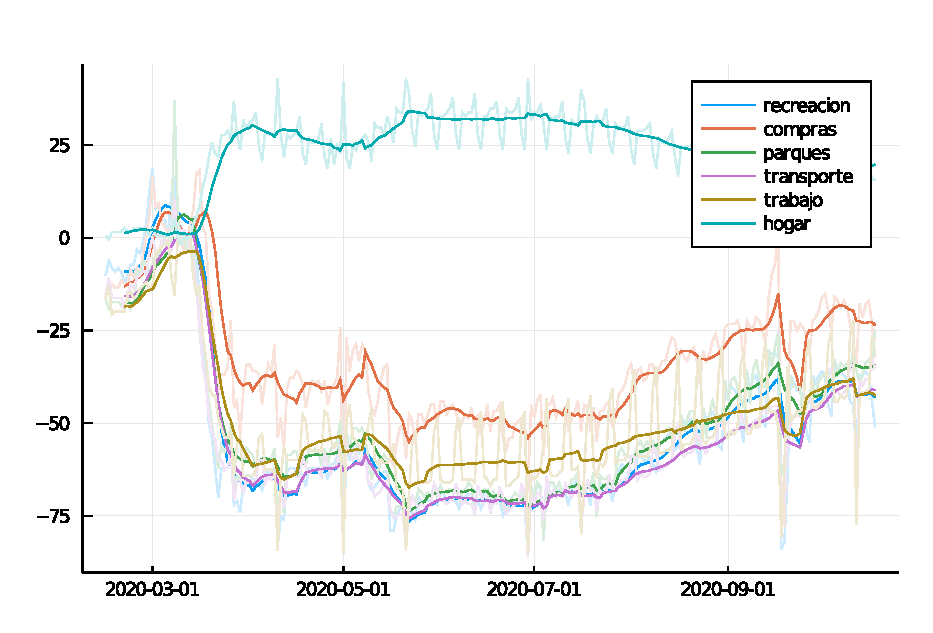
\includegraphics[width=.7\textwidth]{img/metodologia/datos/explorar_movilidad_google_6_1.eps}
\caption{Variación en la movilidad agregada por actividad en la Región Metropolitana y media móvil de 7 días. Fuente: Elaboración propia con datos de Google.}
\label{img:google-movilidad-RM}
\end{figure}


%\noindent \textbf{Uso de infraestructura de telecomunicaciones}
\subsection{Uso de infraestructura de telecomunicaciones}\label{data:isci}

% Acerca de los proveedores
El Instituto Sistemas Complejos de Ingeniería (ISCI), que agrupa a un conjunto de investigadores de varias universidades de Chile con el objeto de generar trabajo científico y desarrollar soluciones para problemas complejos de ingeniería,
% Sus investigadores desarrollan proyectos en las áreas de la Gestión de Operaciones, Ingeniería de Transporte, Optimización y Energía, y otras como Organización Industrial y Medioambiente. Estas áreas comparten herramientas analíticas básicas y se complementan disciplinariamente. 
%[Link ing ISCI, http://ingenieria.uchile.cl/investigacion/centros-y-programas/88242/instituto-sistemas-complejos-de-ingenieria]
 en conjunto con Entel Ocean, la Unidad Digital de Entel, 
compañía de tecnología y telecomunicaciones, recopilaron información acerca del uso de infraestructura de telecomunicaciones.
%Entel:  https://informacioncorporativa.entel.cl/nuestra-compania

% Acerca de la metodologia 
Los datos se encuentran agrupados a nivel de zona censal. La información disponible les permitió deducir la zona hogar, en donde las personas se encuentran frecuentemente en horarios no laborales. Para cada día laboral (lunes a viernes), determinaron el flujo desde cada zona hogar a otras zonas, durante horarios de trabajo. Estos flujos pueden ser dentro de la misma comuna o a otras comunas, y fueron considerados un proxy de la movilidad en Santiago. % Luego, tomaron promedios semanales a nivel de comuna (excluyendo fines de semana) de esos flujos 

Las dos primeras semanas de marzo del 2020, antes de la declaración de la fase 2 de pandemia por COVID-19 en Chile, fueron consideradas como semanas ``base'', siendo una aproximación para la movilidad usual de cada zona \cite{Olivares2020}. Los cambios en movilidad por zona con respecto a esa movilidad base fueron reportados para cada semana, y se encuentran disponibles en el repositorio de la Mesa de Datos del Ministerio de Ciencia, Tecnología, Conocimiento e Innovación \cite{MINCIENCIA}. También pueden verse en el Visor Movilidad en \url{https://covidanalytics.isci.cl/movilidad/visor-movilidad/}, como en la figura \ref{img:ISCI-movilidad-RM}.
%Datos en https://github.com/MinCiencia/Datos-COVID19/tree/master/output/producto51 

La versión completa de estos datos, que contiene información tanto del origen como del destino de los transeúntes, fue analizada en \cite{Carranza2020}. La versión pública de estos datos, sin embargo, solo contiene la movilidad de entrada y salida de cada zona censal/comuna; es posible saber cuánta gente sale y entra a una zona censal o comuna pero no hacia dónde va.

\begin{figure}[H]
\centering
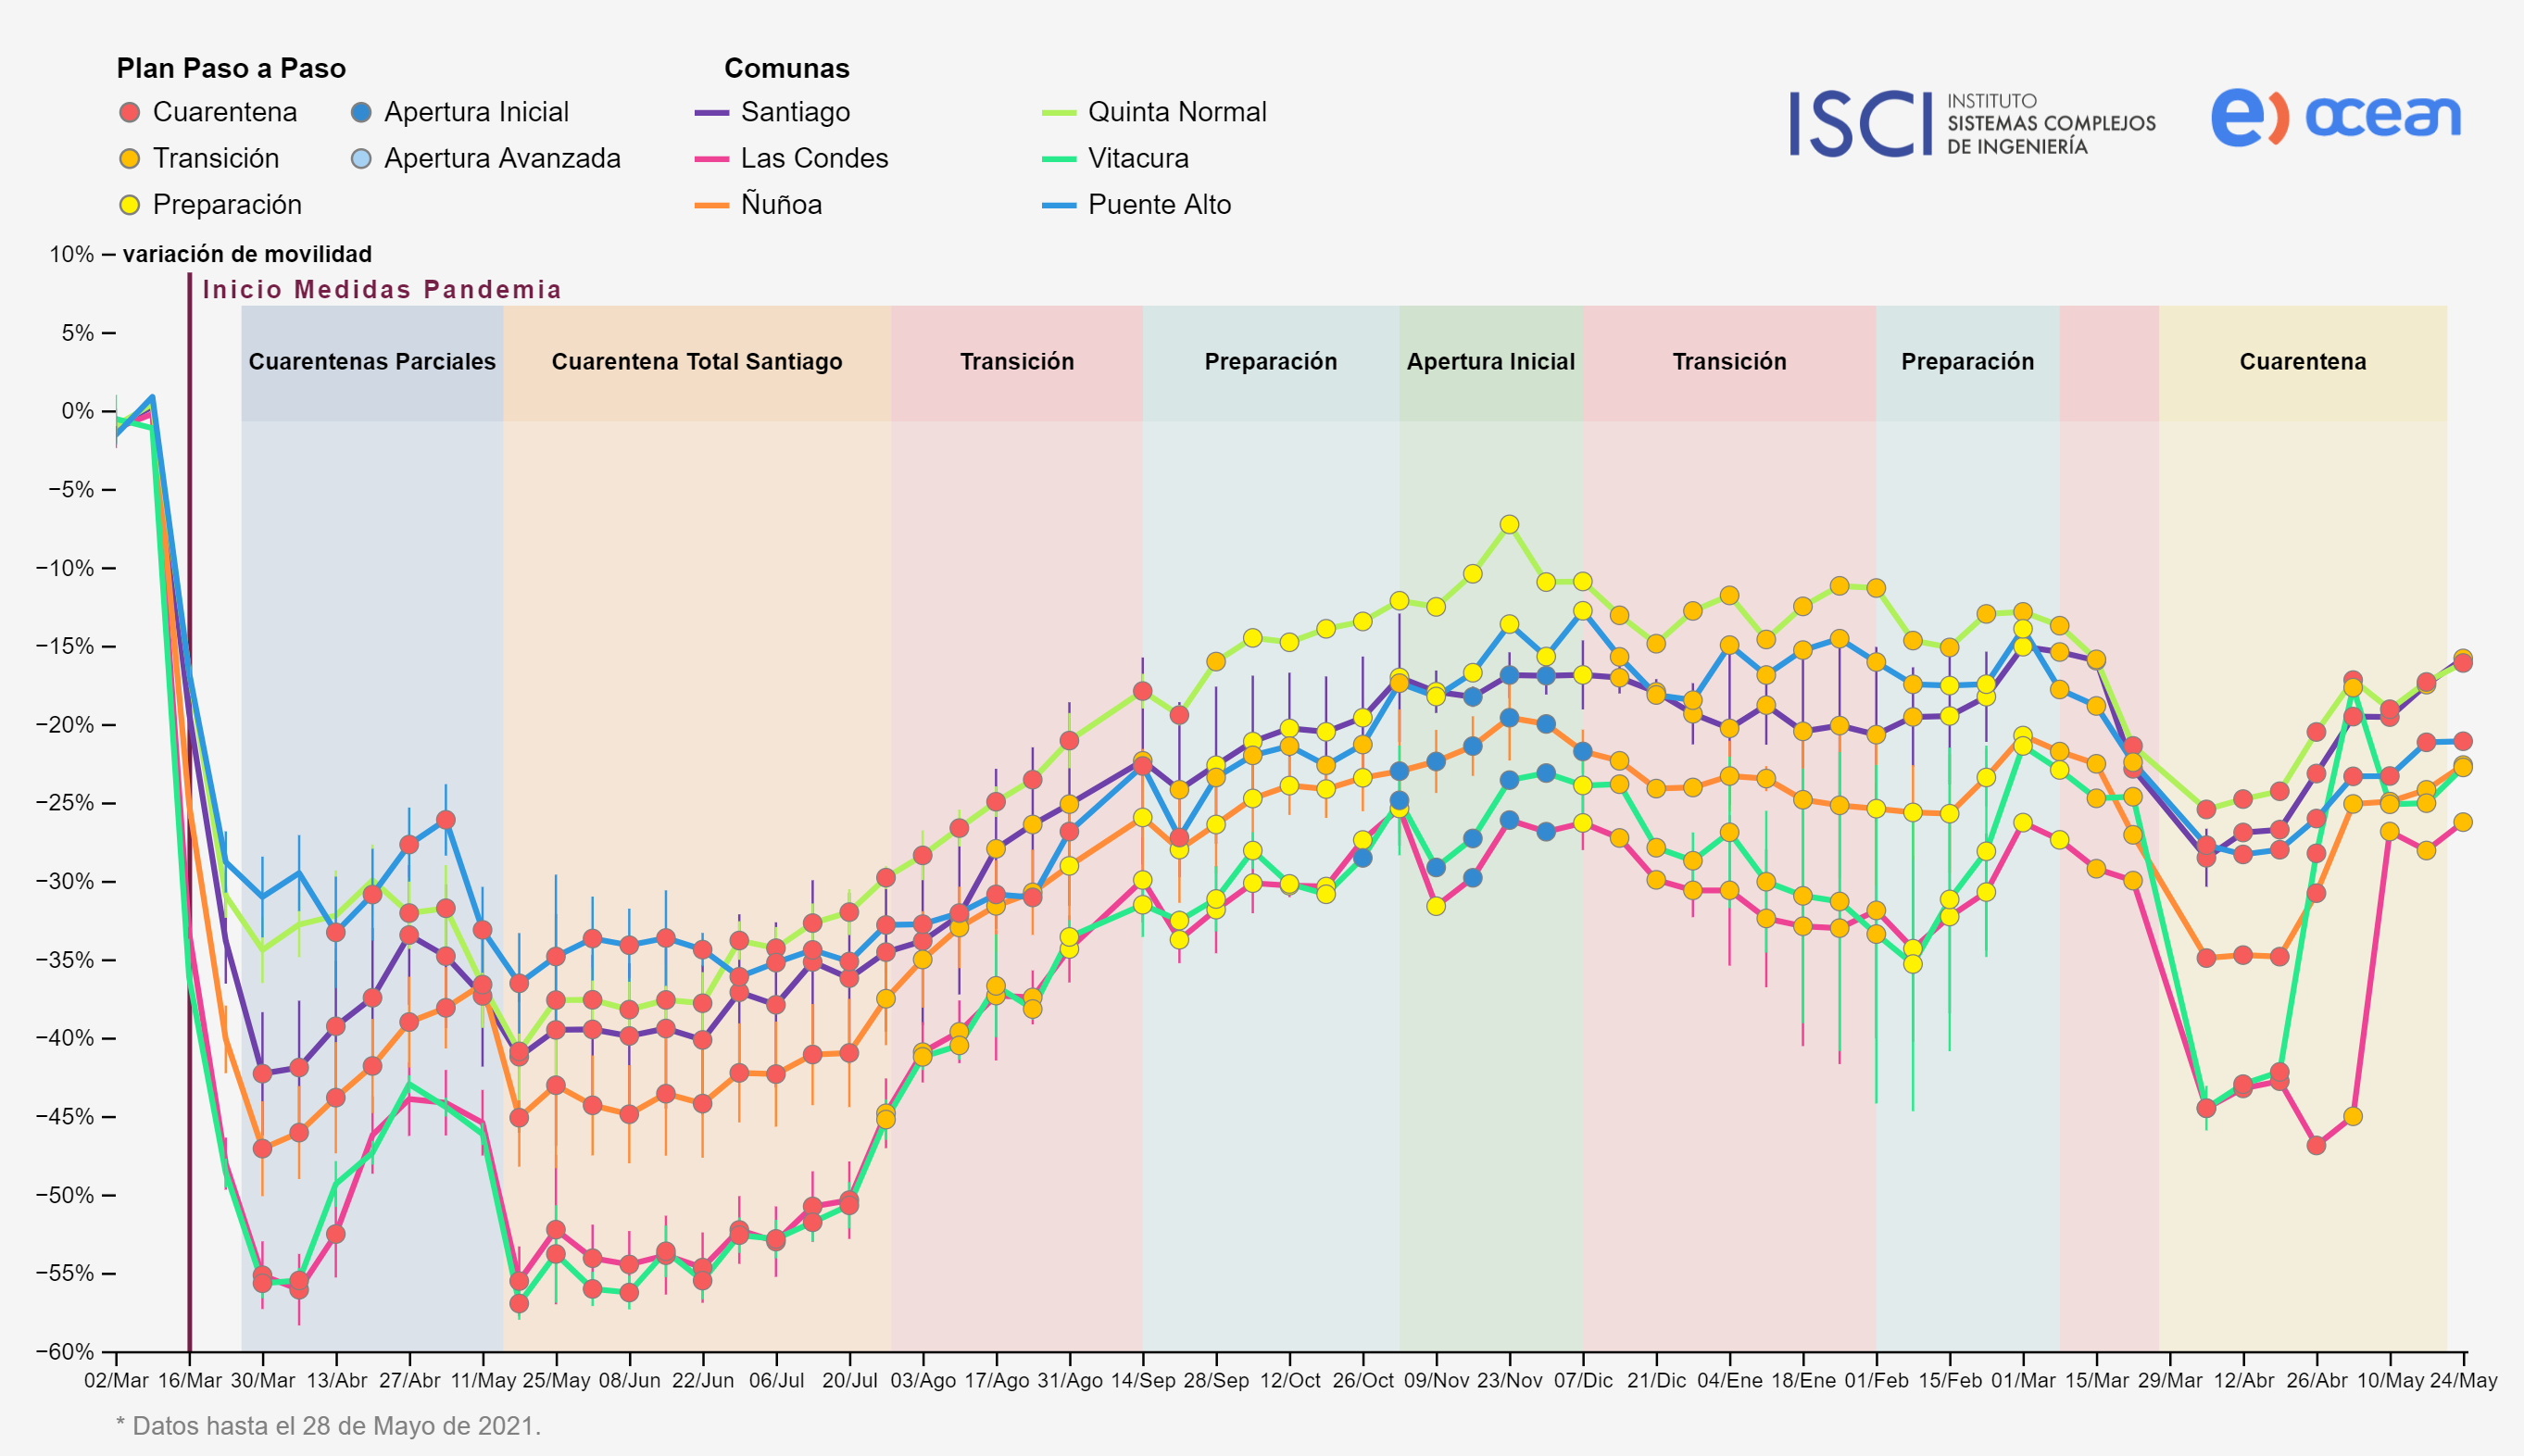
\includegraphics[width=\textwidth]{img/metodologia/datos/ISCI-movilidad-RM.png}
\caption{Variación en la movilidad de seis comunas de la Región Metropolitana. Fuente: ISCI Covid Analytics.}
\label{img:ISCI-movilidad-RM}
\end{figure}




\subsection{Datos-COVID19}\label{sec:datos-minsal}

La Mesa de Datos COVID-19 liderada por el Ministerio de Ciencia, Tecnología, Conocimiento e Innovación busca proveer de información del país durante la pandemia, con el fin de promover el uso de datos para investigación científica, clínica y para soluciones innovadoras. Dispone de datos documentados del Ministerio de Salud (MINSAL) y de otras fuentes \cite{MINCIENCIA}.

% datos disponibles
La información está organizada en distintos \textit{Data Products}. Existen series de tiempo de casos confirmados, hospitalizados, UCI, conectados a ventilación mecánica, fallecidos, cantidad de exámenes PCR realizados, nacimientos y fallecimientos, cuarentenas, etc. Estos datos son utilizados, por ejemplo, en el visualizador del Centro de Modelamiento Matemático disponible en \url{https://covid-19vis.cmm.uchile.cl/geo}. Algunos ejemplos de estos datos son las figuras \ref{img:cmm-fallecidos} y \ref{img:cmm-vacunados}.

\begin{figure}[H]
\centering
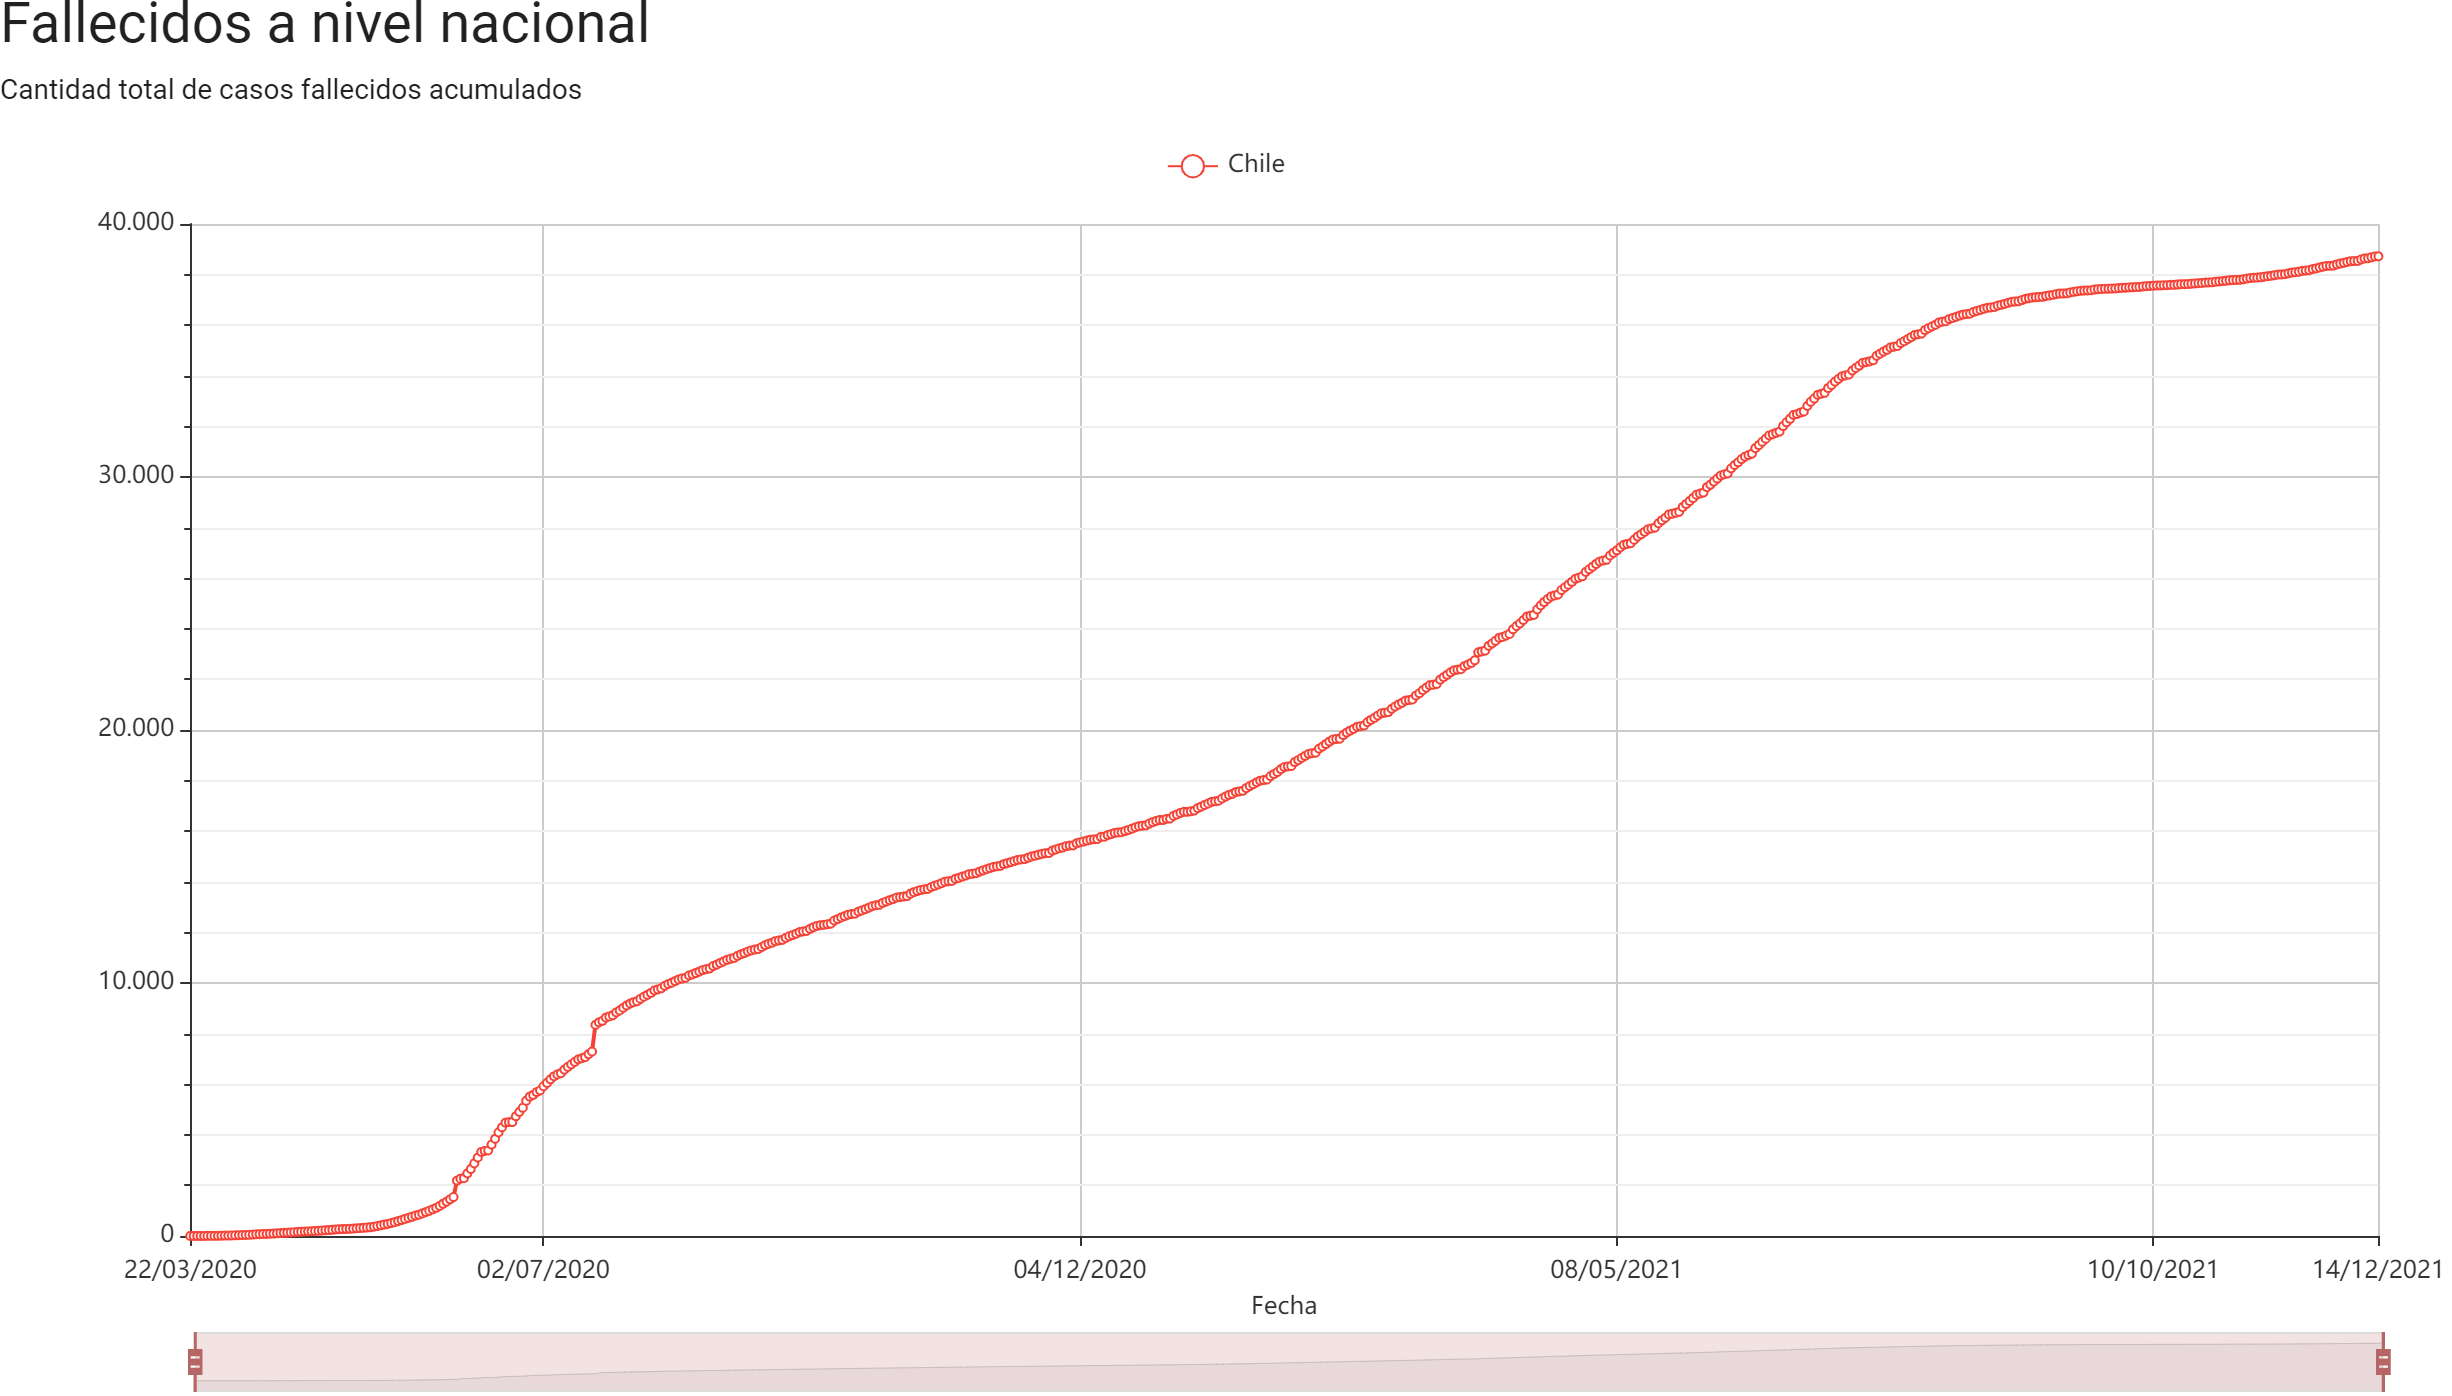
\includegraphics[width=0.9\textwidth]{img/metodologia/datos/fallecidos_nacional.png}
\caption{Total de casos fallecidos por COVID-19 acumulados a nivel nacional. Fuente: Centro de Modelamiento Matemático  con Datos-COVID19.}
\label{img:cmm-fallecidos}
\end{figure}

\begin{figure}[H]
\centering
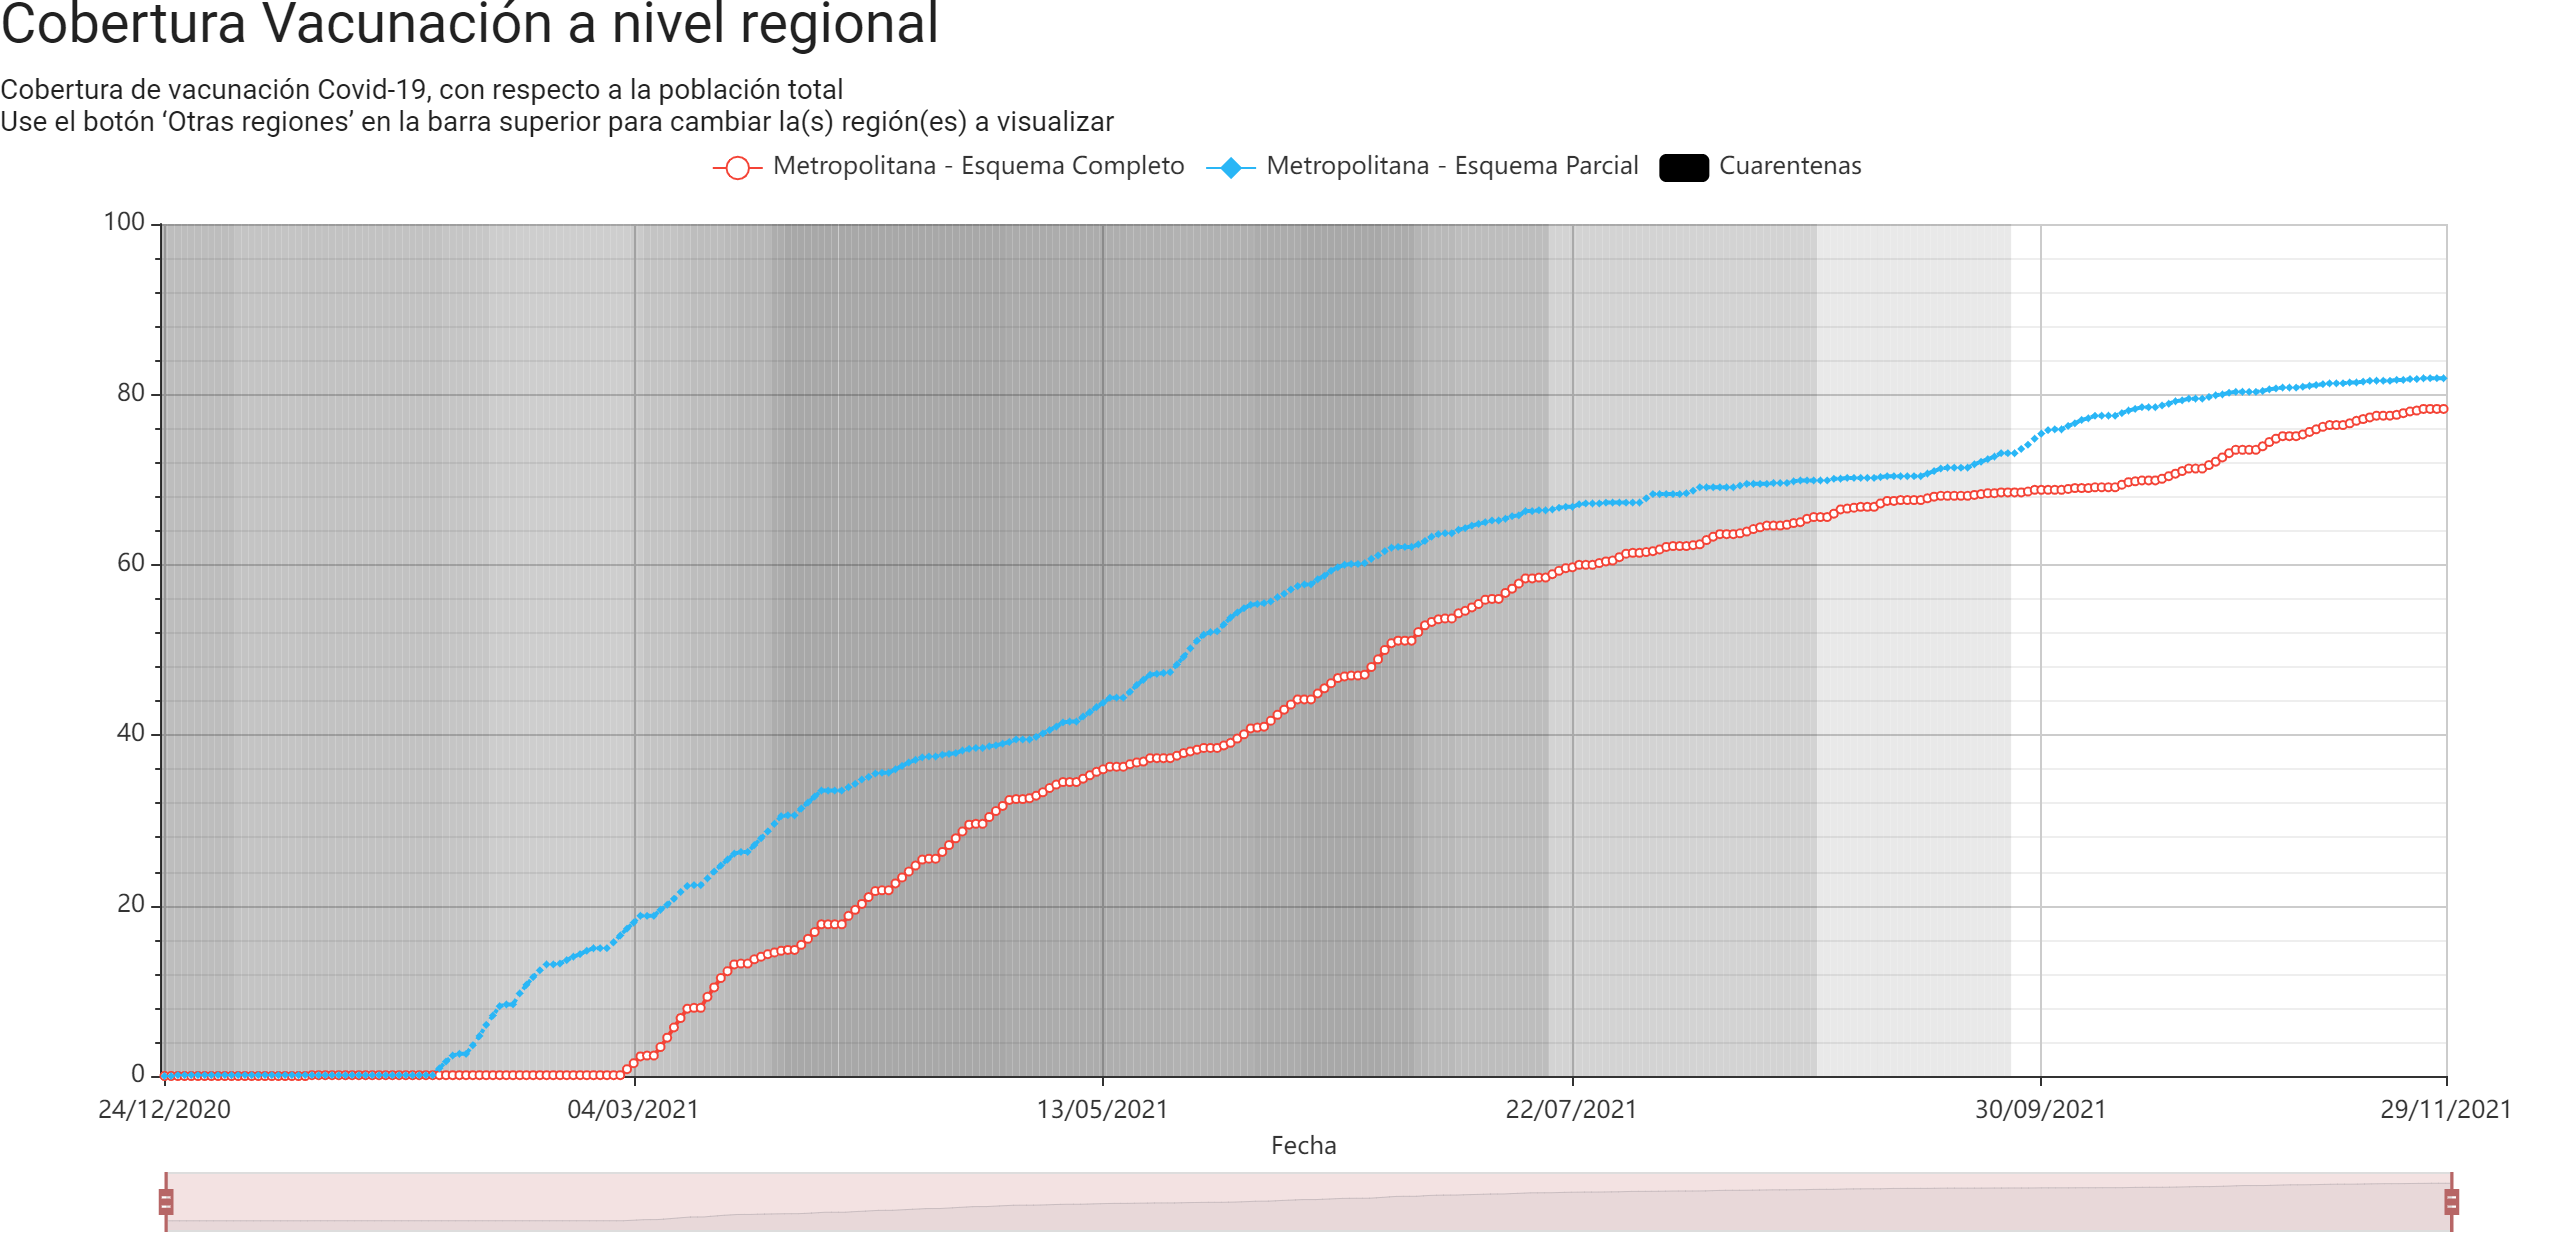
\includegraphics[width=0.9\textwidth]{img/metodologia/datos/CoberturaVacunacionRM.png}
\caption{Porcentaje de cobertura vacunación COVID-19 en la Región Metropolitana. Fuente: Centro de Modelamiento Matemático con Datos-COVID19.}
\label{img:cmm-vacunados}
\end{figure}



% Justificación de la elección de los compartimientos, basada en las características del Covid en la región que estamos estudiando. 
% Modelo multiclase elegido 

\section{Decisiones específicas acerca del modelo} \label{met:decisiones}

% Compartimientos a usar 
% parámetros fijos y variables 

% Todas las decisiones tomadas con respecto a los compartimientos y los parámetros usados van aquí (si se usó uno común para todos, o se ajustaron por separado, etc). 


% describir el modelo que usan en el artículo, como un ejemplo % mencionar las cosas propias del modelo: multiclase, ambientes, tasa de contagio que usa matriz de tiempos de residencia. describir en detalle la tasa de contagio.

% elegir los compartimientos específicos a usar, susceptibles, expuestos, etc. literatura covid

% parametros fijos y variables, literatura covid (ver la parte de kalman, habia algo interesante ahi

% comentar que este modelo permite modelar mascarillas y esas cosas... un avance según pedro 


% Modelos de covid usualmente utilizados (compartimientos, etc)
% Describir este modelo en particular, usando el numero 1. 

% enfoque tasa de contacto vs tiempo de residencia  

% Esto ya lo discutí al inicio 


En esta sección se tomarán decisiones específicas concernientes a la aplicación de la metodología al caso de estudio. Esto permite decidir el modelo específico a utilizar, lo que incluye la elección de compartimientos a utilizar (susceptibles, expuestos, infectados, etc), parámetros, además de las clases y ambientes. Todo esto debe considerar las características del COVID-19 y también los datos disponibles. 

Ya se ha expuesto previamente en \ref{modelo-clases-vs-ambientes} el modelo de dispersión virtual presentado por \cite{Bichara2015}, el cual permite trabajar simultáneamente con clases y ambientes. Ahora se discute las particularidades del modelo a usar en este caso específico. Es necesario definir los compartimientos y parámetros específicos a usar, considerando la enfermedad a modelar, en este caso el COVID-19.
%A continuación se expone el modelo de dispersión virtual con ambientes de \cite{Bichara2015}. Está basado en un modelo de tipo SIS (\textbf{S}usceptibles, \textbf{I}nfectados). 

% acerca de los compartimientos a usar 

Dependiendo del aspecto de interés, distintos compartimentos han sido usados para modelar el COVID-19. Los modelos revisados por la revisión \cite{Xiang2021} utilizan los clásicos Susceptibles, Infectados, Recuperados, en combinación con Expuestos, Hospitalizados y/o Fallecidos. La existencia de casos asintomáticos que portan el virus y pueden contagiarlo pero no presentan síntomas (o presentan síntomas muy leves) es considerado en algunos modelos. Algunos consideran compartimientos En Cuarentena y el desarrollo de vacunas da lugar a modelos con compartimientos de Vacunados.

Como se exponía inicialmente, se buscaba un modelo epidemiológico que considere un riesgo en tres factores: amenaza, exposición y vulnerabilidad. Suponiendo que hay varias clases \(i \in 1 \dots n\) y ambientes \(j \in 1 \dots m\), la idea propuesta de amenaza era de la forma \(\beta_j I_j/N_j\), que incluía la fracción de infectados en un lugar y un factor \(\beta_j\) dependiente de las características del lugar. Se consideraban además valores \(p_{ij}\), que representaban la fracción de tiempo que la clase \(i\) pasaba en el ambiente \(j\), y un factor sanitario \(\alpha_i\) dependiente de la clase \(i\) y relacionado a las medidas de cuidado personal y la susceptibilidad al contagio. Al combinar lo anterior se obtenía la expresión \ref{eq:idea-1}, que da una idea de la tasa de contagios de la clase \(i\) buscada.

\begin{equation}\label{eq:idea-1}
\alpha_i \sum_{j = 1}^m \beta_j p_{ij} \frac{I_j}{N_j}
\end{equation}

Para hacer de esta idea algo concreto, se vuelve al apartado \ref{modelo-clases-vs-ambientes}, donde se habló del modelo de clases y ambientes propuesto por \cite{Bichara2015}\cite{Bichara2018}. Como antess, se separa a la población en \(n\) clases, las cuales interactúan en \(m\) ambientes o áreas de riesgo. \(N_i(t), i = 1, \dots, n\) corresponde a la población de la clase \(i\). Se supone que la población de la clase \(i\) pasa una proporción \(p_{ij} \in [0,1]\) de su tiempo en el ambiente \(j\), con \(\sum_{j = 1}^{m} p_{ij} = 1\) para cada \(i\). Para casos extremos, por ejemplo, podría darse que \(p_{ij} = 0\), es decir, la clase \(i\) no gasta nada de su tiempo en el ambiente \(j\), mientras que \(p_{ij} = 1\) significa que la clase \(i\) pasa todo su tiempo en el ambiente \(j\). La matriz \(P = \{p_{ij}\}_{i = 1\dots n,j \dots m}\) es llamada matriz de tiempos de residencia. Esta matriz será estimada a partir de los datos disponibles. Más aún, se busca una matriz que sea variable en tiempo, de tal forma que refleje los cambios en el comportamiento de la población a lo largo de la pandemia.


Se decide trabajar con el ampliamente utilizado modelo SEIR; ya ha sido utilizado para estudiar el impacto de las cuarentenas y reducciones de movilidad y viajes \cite{Lai2020}\cite{Chinazzi2020}, demás del uso de mascarillas \cite{Kai2020}, por lo que parece una elección razonable. Las ecuaciones del modelo elegido son \ref{eq:modelo-final}. Se decidió despreciar los efectos demográficos de los nacimientos y fallecimientos naturales de la población. Eso se traduce en tasas de natalidad y mortalidad \(b_i, d_i\) iguales a 0. Esto debido a que no se trabajará a largo plazo, solo con un intervalo de tiempo de poco más de un año.

La matriz de tiempos de residencia \(P(t) = \{p_{ij}(t)\}_{i,j}\) será una variable en el tiempo, la forma de estimarla se expondrá en la sección \ref{met:matriz}. Esto se hará de antemano, antes de correr el modelo, por lo que se considera conocida. Se usará la información conocida acerca del COVID-19 para los valores \(\gamma_{Ei}, \gamma_{Ii}\) y los riesgos específicos de cada ambiente \(\beta_j\) se elegirán antes usando valores plausibles. La estimación del factor sanitario \(\alpha_i(t)\) se presentará en \ref{met:estimacion}.

\begin{equation}\label{eq:modelo-final}
\begin{aligned}
%S_i(t)' &= -S_i(t) {\color{Red} \lambda_i(\vec{x}, t) } \\
S_i'(t) &= - \lambda_i(\vec{x}, t)\\
E_i'(t) &= \lambda_i(\vec{x}, t) S_i(t)  - \gamma_{Ei} E_i(t) \\ 
I_i'(t) &= \gamma_{Ei} E_i(t)  - \gamma_{Ii} I_i(t) \\ 
R_i'(t) &= \gamma_{Ii} I_i(t) \\
\lambda_i(\vec{x}, t) &= \alpha_i(t)\sum_{j=1}^m \beta_{j}p_{ij}(t) S_i(t) \left(\frac{\sum_{k=1}^{n}p_{kj}(t) I_k}{\sum_{k=1}^{n}p_{kj}(t)N_k}\right)
\end{aligned}
\end{equation}

Con respecto a los compartimientos elegidos, se decidió no utilizar uno de Fallecidos. Ahora bien, \cite{Mena2021} menciona que al trabajar con niveles socioeconómicos, la cantidad de fallecidos es muchos más confiable que la de casos infectados detectados debido a problemas de trazabilidad en las comunas de menores recursos, especialmente al inicio de la pandemia. El problema es que la tasa de fallecimiento o la fracción de infectados que fallecen es probablemente variable en tiempo, dependiente de las distintas políticas usadas para enfrentar la pandemia. Se decidió mantener la simplicidad del modelo estimando únicamente el factor sanitario. Por motivos similares, la vacunación no fue considerada, sin embargo, se espera que sus efectos se reflejen directamente en el factor sanitario, al hacer a los vacunados menos vulnerables a una posible infección.


% Hay un estudio que calcula Impact of universal masking. 




% Cada ambiente \(j\) tendrá asociado un riesgo \(\beta_j\). Se impone que el riesgo en el ambiente \texttt{hogar} es \(\beta_{\text{hogar}} = 1\). Todos los demás riesgos deben fijarse relativos a ese valor. Se decide incorporar un factor sanitario \(\alpha_i\), dependiente de la clase, el que se interpreta como un indicador del nivel de respeto por las medidas sanitarias (lavado de manos, uso de mascarillas, guardar la distancia, etc) de la clase \(i\)-ésima. Se supone que los efectos de la movilidad están completamente incluídos en la matriz de tiempos de residencia, por lo que este factor solo considera medidas de cuidado. Se supone además que es variable en el tiempo. 


% \[
% \lambda_i(\vec{x}, P) = \alpha \sum_{j=1}^m \beta_{j}p^S_{ij}
% \left(
% p_E \frac{\sum_{k=1}^{n} r^E_{kj}E_k}{\sum_{k=1}^{n}r^E_{kj}N_k} +
% p_{I} \frac{\sum_{k=1}^{n} r^I_{ kj}I_k }{\sum_{k=1}^{n}r^I_{kj}N_k} +
% p_{I^m} \frac{\sum_{k=1}^{n}r^{I^m}_{kj}I^m_k}{\sum_{k=1}^{n}r^{I^m}_{kj}N_k}
% \right)
% \]



% Otras decisiones ... tal vez en otro lugar 
% UNa vez que se deciden las clases y ambientes. 


% Veamos a qué corresponde cada una de las variables. Considero
% $V \in \{S,E,I,I^m\}$.

% \begin{itemize}
% \itemsep1pt\parskip0pt\parsep0pt
% \item
%   $\beta_j$ es una medida de riesgo por unidad de tiempo del ambiente
%   $j$. Yo diría que corresponde a cantidad de contagiados por día en el
%   ambiente $j$, pero no estoy segura. De ser así, se mediría en
%   personas/día.
% \item
%   $p_{ij}^V \in [0,1]$ corresponde a la fracción de tiempo que gastan
%   las personas en el estado $V$ la clase $i$ en el ambiente $j$. Se mide
%   en días.
% \item
%   $p_{kj}^VV_k$ se mide en días $\cdot$ persona. Su valor máximo es
%   cuando $p_{kj}^V = 1$, ahí vale $V_k$ días $\cdot$ persona (son como
%   las horas $\cdot$ hombre, que en economía es una medida de
%   ``esfuerzo'' necesario para llevar a cabo una actividad). Corresponde
%   al tiempo total invertido por todas las personas de la clase $k$ que
%   están en el estado $V$de la enfermedad en el ambiente $j$. Es el
%   ``trabajo de contagio'' del grupo $V_k$.
% \item
%   Es interesante además considerar $p_{kj}^V N_k$, porque no coincide el
%   estado de la matriz $P$ con el que estamos multiplicando. El el
%   ``trabajo de contagio'' que se realizaría si todas las personas de la
%   clase $k$ se movieran como si estuvieran en el estado $V$. El
%   ``trabajo de contagio'' hipotético que realizaría la clase $k$ si
%   estuvieran todos en estado $V$.
% \item
%   Cuando sumamos en todas las clases $k = 1, \dots, n$ obtenemos
%   $\sum_{k=1}^{n}p^{V}_{kj}V_k$, el ``trabajo de contagio'' del estado
%   $V$ realizado en el ambiente $j$.
% \item
%   La suma del denominador $\sum_{k=1}^{n}p^{V}_{kj}N_k$ corresponde al
%   ``trabajo de contagio'' hipotético que se haría en el ambiente $j$ si
%   toda la población estuviera en el estado $V$.
% \item
%   Visto así, creo que el término $\alpha_V$ es una medida de la
%   efectividad del ``trabajo de contagio''. Debería ser un número en
%   $[0,1]$, pero no estoy segura. Aún no tengo clara la unidad de medida.
%   Podría ser como una medida de productividad. La productividad se
%   mide en (cantidad producida)/(horas $\cdot$ hombre). Tiene sentido
%   creo\ldots{} así se anularía después con el término $S_ip_{ij}$, que
%   se mide en (horas $\cdot$ hombre). Lo especial de ese término es que
%   se usa para comparar entre los distintos estados (debería cumplirse
%   $\alpha_I > \alpha_{I^m}> \alpha_{E}$).
% \item
%   Si ahora consideramos la fracción
%   $\frac{\sum_{k=1}^{n}p^{V}_{kj}V_k}{\sum_{k=1}^{n}p^{V}_{kj}N_k}$, lo
%   que tendríamos es una fracción de ``esfuerzo'', sería algo como:
%   ``trabajo real de contagio de $V$ en $j$''/``trabajo ideal de contagio
%   de $V$''. Recalco lo de ``ideal''.
% \item
%   $S_i(t)\lambda_i(\vec{x},P)$ es un flujo, la tasa a la que se pasa del
%   estado $S$ al estado $E$. Se mide en personas/tiempo. No queda otra
%   alternativa entonces de que el término $\beta_j \alpha_V$ se mida en
%   días$^{-2}$. Eso es extraño\ldots{} debería ser un término de
%   aceleración y no de velocidad como pensé al principio. Eso me da la
%   idea de calcular $S''_i(t)$\ldots{} pero no me llevó muy lejos.
% \item
%   Necesito setear algún valor. Digamos que $\alpha_I = 1$. Luego,
%   $\beta_j p_{ij} \alpha_{I} \frac{\sum_{k=1}^{n} p^I_{ kj}I_k }{\sum_{k=1}^{n}p^I_{kj}N_k}$
% \item
%   Necesito llevar esa cantidad a contagios/tiempo. Necesito una medida
%   de la eficiencia del trabajo de contagio. Eso debería medirse en
%   contagios/(hora $\cdot$ persona).
% \end{itemize}


% Elección de matriz de tiempos de residencia 
% Cómo variarla en el tiempo (sección por trabajar)
% Justificación de la elección de ambientes, basada en los que hayan sido importantes, los que aparecen en los datos, etc. 
\section{Matriz de tiempos de residencia}\label{met:matriz}

En la sección anterior se planteó el modelo multiclase con dispersión virtual. La principal diferencia con respecto a otros modelos multiclase estaba en la forma en que se calculaba la tasa de contagio; las \(n\) clases interactúan en \(m\) ambientes virtuales. Esta interacción está codificada por medio de la matriz de tiempos de residencia \( \mathbf{R} =\{r_{i,j}\}_{i \in 1 \dots n, j \in 1 \dots m}\), donde la entrada \(r_{ij}\) corresponde a la fracción del día que la clase \(i\) pasa en el ambiente \(j\).

El objetivo de este apartado es elegir las clases y ambientes a utilizar para estudiar el caso de Santiago, y estimar la matriz \(\mathbf{R}\) de tiempos de residencia asociada. Es importante notar que esta matriz será variable en el tiempo, puesto que las diferentes medidas de mitigación (cierre de instituciones educativas, cuarentenas) implementadas por el gobierno de Chile ([link]) han cambiado significativamente el modo de vida en la ciudad.  

Se comienza eligiendo las clases y ambientes a utilizar. Posteriormente, se describirá la metodología para la obtención de una matriz de tiempos de residencia \(\mathbf{R}^0\) correspondiente a la ciudad de Santiago en condiciones normales. Finalmente se describirá la metodología para modificar esta matriz, con el fin de reflejar las variaciones en el comportamiento de la población a lo largo del desarrollo de la pandemia, lo que da lugar a la matriz \(\mathbf{R}(t)\) definitiva.


\subsection{Elección de clases y ambientes}

Hay varios criterios a considerar a la hora de elegir las clases y los ambientes. En primer lugar, es ampliamente conocido \cite{} que la edad es un factor importante en el efecto de la enfermedad en una persona; el Covid19 afecta con más intensidad a los adultos mayores. Varios estudios \cite{} % alguno internacional 
\cite{Mena2021}\cite{Bennett2021} han mostrado que la pandemia ha afectado más fuertemente a los niveles socioeconómicos o comunas más pobres y lo asocian, entre otras cosas, a la dificultad de ellos de acatar las cuarentenas. Se ha mencionado también el sexo como una variable a tener en cuenta \cite{}, y la Encuesta Origen Destino muestra diferencias en el uso del tiempo entre hombres y mujeres \cite{Jara-Diaz2013}.

Los datos disponibles han de ser considerados también. La Encuesta Origen Destino, por un lado, posee datos muy granulares; es posible conocer para un individuo su sexo, zona censal y comuna donde reside, edad e ingreso familiar. Más aún, los distintos propósitos de los viajes realizados (regreso al hogar, al trabajo, escuela, compras, transporte público, bicicleta, entre otros) entregan varios ambientes donde ese individuo pasa su tiempo. 

Por otro lado, las demás fuentes de datos no poseen tanta información. El Uso de infraestructura de telecomunicaciones permite conocer cómo ha cambiado la movilidad de entrada o salida a cada zona censal/comuna, pero no distingue entre las actividades que realizan las personas mientras se mueven por la ciudad. Los Informes de Movilidad Local sobre Covid19 de Google permiten distinguir distintas actividades, pero no permiten separar por comuna.

Las series de tiempos de Datos-COVID19 presentan dificultades similares. Están desagregadas por edad, sexo o comuna, pero no por los tres criterios simultáneamente.

Puesto que se desea considerar el efecto de las cuarentenas en el uso del tiempo de las personas a lo largo de la pandemia, sabiendo la importancia que juega en las diferencias entre las distintas comunas, se decide usar los datos de Uso de infraestructura de telecomunicaciones. Esto lleva a desechar la información de los distintos ambientes; se sabe que hay más o menos movilidad fuera del hogar, pero no se sabe exactamente en qué actividad. El trabajo considera, por tanto, solo \(m = 2\) ambientes: \texttt{hogar} y \texttt{exterior}. Siguiendo a \cite{Ferguson2020}, el número de contagios en el hogar es aproximadamente de 1/3, por lo que, ya que se fijó \(\beta_{\text{hogar}} = 1\), se supondrá que \(\beta_{\text{exterior}} \approx 2\).

Los datos elegidos permiten utilizar la información a nivel de zona censal, pero los datos epidemiológicos no son tan granulares, por lo que es más factible distinguir por comuna. Los datos epidemiológicos están disponibles a este nivel también, por lo que es una buena posibilidad. Eso, sin embargo, plantearía un sistema con unas 50 clases, lo que para 4 compartimientos da unas 200 variables. Es posible, aunque agrega más carga computacional y dificulta el análisis posterior. Se decide, por simplicidad, reducir el análisis a \(n = 5\) categorías socioeconómicos, las mismas propuestas por \cite{SEREMIRM2019}, que surgen tras ordenar las comunas por IPS. Pueden verse en la Tabla \ref{table:ips-categ}.

Ante la falta de la información adecuadamente desagregada para edad y sexo, se decide abandonar estos criterios.

% Agregar población según CENSO 
\begin{table}[h!]
\centering
\begin{tabular}{|c c c c|} 
 \hline
 \textbf{Prioridad Social} & \textbf{IPS mínimo} & \textbf{IPS máximo} & \textbf{Ejemplos} \\ [0.5ex] 
 \hline
 Alta & 78.24 & 83.03 & La Pintana, Lo Espejo\\ 
 Media Alta & 73.84 & 77.39 & San Bernardo, El Bosque\\
 Media Baja & 65.05 & 71.36 & La Cisterna, Quinta Normal\\
 Baja & 53.34 & 64.37 & Santiago, Providencia\\
 Sin Prioridad & 6.26 & 37.36 & Las Condes, Lo Barnechea\\ [1ex] 
 \hline
\end{tabular}
\caption{Categorías socioeconómicas de IPS dadas por \cite{SEREMIRM2019}.}
\label{table:ips-categ}
\end{table}

\subsection{Matriz de Santiago en condiciones normales} 

% Acerca de los propósitos de viajes 
% Los propósitos son los siguientes:
% Al trabajo
% Por trabajo
% Al estudio
% Por estudio
% De salud
% Visitar a alguien
% Volver a casa
% Buscar o Dejar a alguien
% Comer o Tomar algo
% Buscar o dejar algo
% De compras
% Trámites
% Recreación
% Otra actividad 
En \cite{Munizaga2011} se propone un método para obtener información acerca del uso del tiempo de una persona a partir de los tiempos de inicio y fin de sus viajes, contenidos en la Encuesta Origen-Destino, y el propósito declarado de este. Para esto supone que el primer viaje comienza desde el hogar (esto puede verificarse revisando que calcen la zona de origen del viaje con la del hogar). Luego, a cada período de tiempo entre dos viajes consecutivos es asignado a la actividad declarada como propósito en el viaje anterior. La Figura \ref{img:ciclo-viajes} es un diagrama de este proceso. El Algoritmo \ref{alg:timematrix} explica el proceso en detalle de manera general, agregando además ambientes para los distintos modos de transporte. La matriz obtenida usando este algoritmo se denota \(\mathbf{R}_0\). La matriz variable en el tiempo será construida a partir de esta en la siguiente subsección.
% Insertar el algoritmo para esto, traducir 

\begin{figure}[H]
\centering
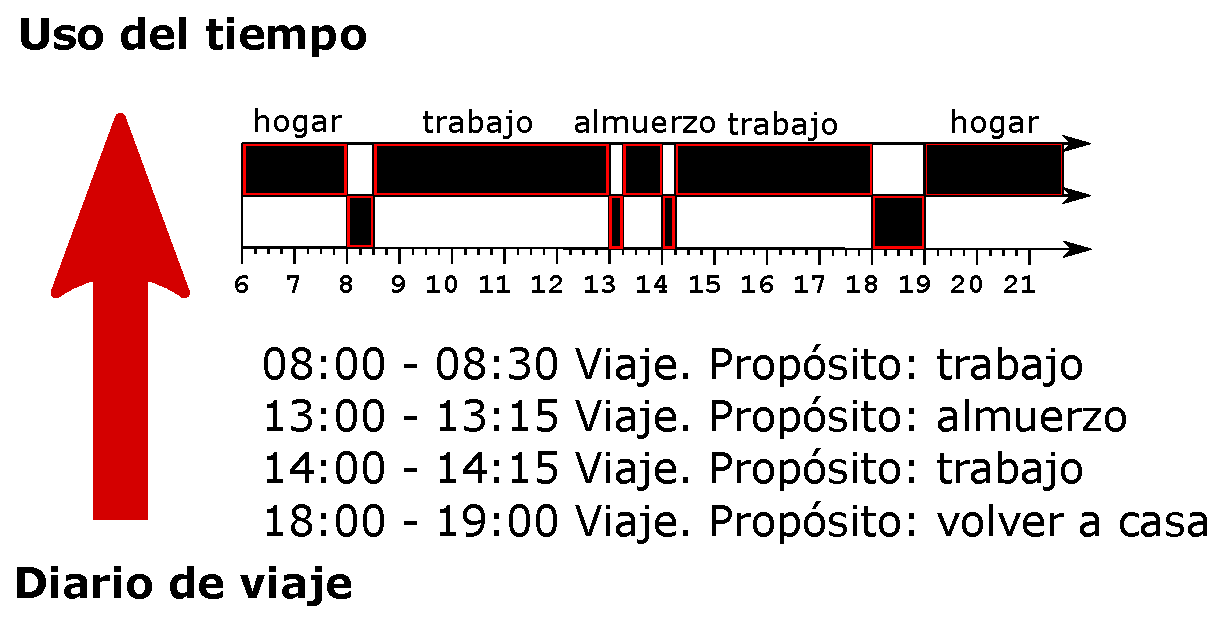
\includegraphics[width=.6\linewidth]{img/metodologia/matrizPnormal/ciclo-viajes.eps}
\caption[Transformar propósitos de viaje en tiempo de actividad.]{Transformar propósitos de viaje en tiempo de actividad. Fuente: \cite{Munizaga2011}, traducción propia.}
\label{img:ciclo-viajes}
\end{figure}

\begin{algorithm}[H]
\SetAlgoLined

\KwIn{
Una lista de personas \(P\). Para cada \(p \in P\), una lista \(V_p\) de todos los viajes hechos por \(p\), ordenados del primero al último. Para un viaje \(v\) es posible obtener \(t_0, t_f\) tiempos de inicio y fin, \(\mathtt{modo}\) de transporte y \(\mathtt{propósito}\) del viaje.
Dos funciones \( \mathcal{J}_{\mathtt{m}}: \mathtt{modo} \mapsto j\) y \(\mathcal{J}_{\mathtt{p}}: \mathtt{propósito} \mapsto j\) que asocian cada \texttt{modo} de transporte (bus, auto, etc) y cada \texttt{propósito} de viaje (al trabajo, de compras, etc) a un ambiente \(j \in \{1, \dots, m\}\) (trabajo, compras, transporte público, etc). Un ambiente por defecto \(j_0\) (hogar), donde las personas sin viajes pasan su tiempo, y donde las personas comienzan su primer viaje. Una función \(\mathcal{C}: p \in P \mapsto i\) que asigne a cada persona \(p\) una clase \(i \in \{1, \dots, n\}\). Tiempos de inicio \(T_0\) y fin \(T_f\) del intervalo de tiempo total considerado.
}

\KwResult{Una matriz de tiempos de residencia \(R = (r_{ij})_{i = 1 \dots n, j = 1 \dots m}\) donde \(r_{ij}\) es la fracción del tiempo que la clase \(i\) pasa en el ambiente \(j\). Solo considera personas sin viajes inválidos.}

%Elegir un grafo $G$ conexo y una matriz $R$. 

Definir la matriz auxiliar \(C = (c_{ij})_{i = 1 \dots n, j = 1 \dots m}\). \(c_{ij}\) guardará el tiempo total que las personas de la clase \(i\) pasan en el ambiente \(j\). Se inicializa en \(0\)\;

Definir \(T = T_f - T_0\) el tiempo total considerado.

Definir \(N_i \gets 0\) para cada \({i \in 1 \dots n}\) para contar el total de personas en cada clase. 

\ForAll{\(p \in P\)}{
    Guardar en \(i\) el valor \(\mathcal{C}(p)\), la clase de \(p\)\; %\tcc*[r]{class of person \(p\)} \;

    \uIf{La persona \(p\) no tiene viajes, \(V_p = \varnothing\)}{
        Se supone que \(p\) pasa todo su tiempo en el ambiente \(j_0\) por defecto. \(c_{i,j_0} \gets c_{i,j_0} + T\)\; 
        
        Contabilizar una persona válida. \(N_i \gets N_i + 1\)\;
    }
    \uElseIf{\(V_p\) tiene información faltante (\(\mathtt{propósito}, \mathtt{modo}, t_0\) or \(t_f\) de algún \(v \in V_p\) no está definido)}{
        \(p\) no es una persona válida y no es considerada en la matriz final\;
    }
    \Else{
        \(j\_\mathtt{anterior} \gets j_0 \). Ambiente donde terminó el viaje anterior. Comienza en \(j_0\)\;
        \(t_f\_\mathtt{anterior} \gets T_0\). Hora de término del viaje anterior. Vale \(T_0\) por defecto\;
        \ForAll{viaje \(v \in V_p\)}{
            Obtener \(\mathtt{prop\'osito}, \mathtt{modo}, t_0\) y \(t_f\) asociados al viaje \(v\). Definir \(j_v \gets \mathcal{J}_\mathtt{m}(\mathtt{modo})\) el ambiente asociado al modo del viaje \(v\)\;
            
            Agregar el tiempo entre el viaje anterior y el viaje \(v\) al ambiente donde terminó el viaje anterior. \(c_{i, j\_\mathtt{anterior}} \gets c_{i, j\_\mathtt{anterior}} + t_s - t_f\_\mathtt{anterior}\)\;
            
            Agregar el tiempo del viaje \(v\) a su ambiente asociado. \(c_{i, j_v} \gets c_{i, j_v} + t_f - t_s\)\;
            
            Actualizar  \(j\_\mathtt{anterior} \gets \mathcal{J}_{\mathtt{p}}(\mathtt{prop\'osito})\). El próximo viaje comienza donde \(v\) terminó.
            
            Actualizar \(t_f\_\mathtt{anterior} \gets t_f\). 
        }
        
        Agregar el tiempo entre el último viaje y el tiempo final \(T_f\) \(v\) al ambiente donde terminó el último viaje. \(c_{i, j\_\mathtt{anterior}} \gets c_{i, j\_\mathtt{anterior}} + T_f - t_f\_\mathtt{anterior}\)\;
        
        Contabilizar a \(p\) como una persona válida. \(N_i \gets N_i + 1\)\;
    }
    
}

Calcular \(R\) a partir de \(C\) normalizando cada fila. \(r_{ij} \gets c_{ij} / T N_i\)\;

\caption{Tiempos de residencia a partir de una lista de viajes}
\label{alg:timematrix}
\end{algorithm}

% Creo que sería bueno agregar el pseudo código de la cuestión. Estoy segura de que yo tenía una versión bonita de esto.
% Para que sea replicable tengo que incluir todas las pequeñas decisiones... los casos usados y los no usados, todo eso. 

% Proceso de manera diferenciada a los no viajeros de los viajeros. Se asume que los primeros pasan todo su tiempo en el hogar. 

% Redirigir a la imeplementación en Matlab.


\subsection{Variaciones de la matriz a lo largo del tiempo} 

% Explicar los datos disponibles
Se usan los datos de movilidad obtenidos del Uso de infraestructura de telecomunicaciones, descritos en \ref{data:isci}. Los datos se obtienen del repositorio de Datos-COVID19, descrito en \ref{data:minciencia}, del Producto 82 específicamente. 
% Nos estoy segura de qué tanto detalle tengo que dar aquí, puedo ser muy específica y describir hasta las columnas involucradas. Tal vez como un anexo... 

Los datos se encuentran en dos archivos en formato \texttt{.csv}, correspondientes a la movilidad durante días de la semana laborables \texttt{ISCI\_weeks.csv} y a la movilidad de los fines de semana \texttt{ISCI\_weekends.csv}. Se usa el primero de estos. Los atributos incluyen la comuna de la Región Metropolitana con nombre \texttt{nom\_comuna} y código único territorial \texttt{comuna} a la que corresponde la medición, semana epidemiológica \texttt{semana} de la medición con fecha de inicio \texttt{fecha\_inicio} y fin \texttt{fecha\_termino}, y estimaciones de la variación de movilidad \texttt{var\_salidas}, que es un promedio entre \texttt{var\_salidas\_cota\_superior} y \texttt{var\_salidas\_cota\_inferior}. 

Se utiliza la información de \texttt{var\_salidas} (despreciando las cotas inferiores y superiores). Si llamamos \(m_i^0\) a la movilidad de referencia inicial para la comuna \(i\)-ésima (la cual es desconocida), y \(m_i^k\) a la movilidad de la comuna \(i\)-ésima en la semana \(k\)-ésima posterior a esa semana de referencia, entonces \texttt{var\_salidas} reporta los valores \(p_i^k\), donde 

\[
m_i^k = p_i^k m_i^0
\]

Un detalle a considerar es que necesario calcular la variación de movilidad para los distintos grupos socioeconómicos, puesto que solo la tenemos para las comunas. Si la población de la comuna \(i\)-ésima es \(N_i\), e \(I\) es un conjunto de comunas, estimamos la movilidad grupal como 
\[
m^k_I = \sum_{i \in I}m^k_i N_i
\]

Buscamos un parámetro \(p_I^k\) tal que 
\[
m_I^k = p_I^k m_I^0
\]

Bajo el supuesto \(m_i^0 := m^0\) para cada \(i\), entonces es fácil ver que

\[
p_I^k = \sum_{i \in I} p_i^k N_i
\]

Supondremos que la movilidad es constante a lo largo de la semana (incluyendo fines de semana). Se define una función \(\mathtt{semana}(t)\) que a un tiempo \(t\) le asocia la correspondiente semana. Suponemos además que el tiempo que cada clase pasa en el ambiente \texttt{exterior} varió de manera proporcional a la movilidad. Eso permite calcular la columna \texttt{exterior} de la matriz de tiempos de residencia para cada grupo socioeconómico \(I\) como

\[
r_{I, \text{exterior}}(t) = p_I^{\mathtt{semana}(t)} r_{I,\text{exterior}}^0
\]

%% Definir una variable para el nombre del ambiente fuera del hogar o exterior 



% Finalmente la matriz de tiempos de residencia que varía en el tiempo 

Finalmente, el tiempo que no se ocupa en el ambiente \texttt{exterior} se pasa en el ambiente \texttt{hogar}, por lo que 
\[
r_{I, \text{hogar}}(t) = 1 - r_{I,\text{hogar}}(t)
\]

% Estimación de parámetros 
\section{Estimación de parámetros} \label{met:estimacion}

% Criterios a considerar... algunos deben ser constantes y otros variables. 

\subsection{Filtro de Kalman}


%Por qué filtro?
Para hacer estimación de parámetros \textit{online} hay varias opciones disponibles; Filtro de Mínimos Cuadrados Recursivo (\textit{Recursive Least Squares}) y su extensión el Filtro de Kalman, permiten estimar un estado a partir de su dinámica  y mediciones de alguna variable. Hay alternativas como el filtro de partículas, más costoso computacionalmente, o el filtro por ensambles. Cada uno tiene su propias deficiencias [referencias]. 

% por qué kalman? No un filtro de partículas? EnkF por qué no? H_infty?



%Filtro de Kalman para sistemas continuos no lineales
%Hay muchas alternativas, por qué usar el filtro extendido existiendo también UKF o CKF? No se necesitaba tanto poder de cómputo tampoco...

Filtro de Kalman fue desarrollado en primera instancia como un método para tratar sistemas lineales discretos [verificar]. No hay una única forma de trabajar con sistemas continuos no lineales; por una parte, es posible discretizar el sistema mediante métodos como Euler o Runge-Kutta, para luego tratar la no linealidad (este método es llamado \textit{discreto-discreto} en \cite{Kulikov2014}. Por otra parte, es posible linealizar el sistema primero, lo que da lugar al filtro \textit{continuo-discreto}.

Tratar con la no linealidad del sistema puede hacerse de varias formas. La más directa es simplemente linealizar, lo que da lugar al Filtro de Kalman Extendido (EKF por sus siglas en inglés). Hay enfoques más sofisticados que funcionan mejor para problemas altamente no lineales como el \textit{Unscented Kalman Filter} (UKF) (Filtro de Kalman ``sin olor'') o el \textit{Cubature Kalman Filter} (CDF) que se basan estimar la media y varianza de una distribución a la que es aplicada una función no lineal, mediante la evaluación de esa función en varios puntos estratégicamente elegidos, llamados \(\sigma\)-puntos \cite{Kulikov2017}\cite{Simon2006}. Por simplicidad de la implementación y a la hora de chequear observabilidad local, se decidió utilizar EKF en su versión discreta-discreta. La misma decisión fue tomada por \cite{Hasan2020}, pero se prefirió utilizar una discretización de Runge-Kutta de orden 4 en lugar del método de Euler progresivo por estabilidad numérica.


%Por qué usar smoother, qué pasa al usar kalman normal, etc, en qué situaciones habría que usaar kalman... (forecasting por ejemplo).

Debido a que se trabajará con datos pasados y no se hará estimación \textit{online} ni predicción, se utiliza suavizado en lugar de filtraje [referencia a 2.2]. El suavizado será de intervalo fijo, como se explica en [2.2.5], y se usará su versión más conocida, el \textit{Rauch, Tung y Striebel Smoother} o \textit{RTS Smoother} \cite{}\cite{Simon2006}. Esto permite obtener mejores estimaciones, pero solo es posible debido a que disponemos de todas las observaciones para un intervalo de tiempo fijo, y que deseamos la mejor estimación posible dadas esas observaciones. Para estimación \textit{online} solo se cuenta con las mediciones hasta el intervalo donde se quiere estimar, no hay observaciones futuras, lo que lleva a usar filtraje.



\subsection{Modelo}

Para fijar ideas, se comienza con un modelo de una sola clase 
\begin{equation}
\begin{aligned}
S'(t) &= -\alpha S(t)\big( p_E E(t) + p_{I^m}I^m(t) + p_I I(t)\big) \\
E'(t) &= \alpha S(t)\big( p_E E(t) + p_{I^m}I^m(t) + p_I I(t)\big) - \gamma_E E(t) \\ 
(I^m)'(t) &= (1-\phi) \gamma_E E(t) - \gamma_{I^m} I^m(t)\\
I'(t) &= \phi \gamma_E E(t) - \gamma_{I} I(t)\\
R'(t) &= \gamma_{I} \big( I^m(t) + I(t) \big)
\end{aligned}
\end{equation}

donde, como de costumbre, \(S\) corresponde a los susceptibles, \(E\) a los expuestos, \(I^m\) a los infectados sintomáticos, \(I\) a los infectados sintomáticos y \(R\) a los recuperados. \(\gamma_E\) corresponde a la tasa de salida de ... medida en \([\text{día}]^{-1}\), de tal forma que \(\gamma_E^{-1}\) es el período de incubación medido en \(\text{día}\)s. \(\gamma_{I^m}\) y \(\gamma_I\) corresponden a las tasas de recuperación de los infectados asintomáticos y sintomáticos respectivamente. \(\phi\) es la fracción de infectados que son sintomáticos. Consideraremos \(\alpha\) como proporcional a la tasa de contagios.

\subsection{Estimación de la tasa de contagios}

Siguiendo la misma línea que \cite{Hasan2020}, \cite{Hasan2021}, \cite{Hasan2021a}, supondremos que \(\gamma_E\) y \(\gamma_I\) son constantes y que \(\alpha(t)\) es variable y depende de las distintas medidas sanitarias implementadas.


Se cuenta con datos de los casos sintomáticos acumulados, que se calculan como 

\[
C_i(t) = \int_{t_0}^t \gamma_E E_i(s) ds
\]

\noindent \textbf{Modelo con una clase}

Para fijar ideas, se trabaja con el modelo SEIR clásico de una sola clase, incorporando ruido:

\begin{equation}
\begin{aligned}
S'(t) &= -\alpha(t) S(t)I(t) + g_1 w_1(t)\\
E'(t) &= \alpha(t) S(t)I(t) - \gamma_E E(t) + g_2 w_2(t)\\
I'(t) &= \gamma_E E(t) - \gamma_{I} I(t) + g_3 w_3(t)\\
R'(t) &= \gamma_{I} I(t) + g_4 w_4(t)\\
\end{aligned}
\end{equation}

\(w_1, \dots, w_4\) son procesos brownianos independientes entre sí, ponderados por constantes \(g_1, \dots, g_4\).
Se supondrá que \(\gamma_E, \gamma_{I^m}\) y \(\gamma_I\) son conocidos, y se busca estimar \(\alpha(t)\) a partir de observaciones ruidosas de los casos infectados acumulados. Se trabajará con un modelo aumentado, agregando las ecuaciones \ref{eq:simple-augmented-eqs} a la dinámica. \ref{eq:simple-c} permite guardar los casos acumulados en un estado, lo que facilita plantear la ecuación de observación. \ref{eq:simple-alpha} agrega \(\alpha\) a la dinámica sin ser modificada por ella, de forma que solo es actualizada por el paso de análisis del filtro de Kalman.

\begin{subequations}\label{eq:simple-augmented-eqs}
\begin{align}
C'(t)       &= \gamma_E E(t) \label{eq:simple-c} \\ 
\alpha'(t)  &= 0    \label{eq:simple-alpha}
\end{align}
\end{subequations}

Llamando \(\mathbf{x} = (S, E, I, R, C, \alpha)^{\top}\), se obtiene la ecuación de estado \ref{eq:simple-estado}, con parámetros conocidos \(p = (\gamma_E, \gamma_I)\). \(\mathbf{G}\) es una matriz diagonal que pondera el ruido, y \(\mathbf{w}\) un vector de brownianos independientes. Si bien \(f_p\) no depende del tiempo de manera explícita, al trabajar con el modelo completo si habrá dependencia, por lo que se decidió escribir \(f_p(\mathbf{x}, t)\) en lugar de simplemente \(f_p(\mathbf{x})\).

\begin{equation} \label{eq:simple-estado}
\mathbf{x}'(t) =
\begin{pmatrix}
S \\
E\\
I\\
R\\
C\\
\alpha 
\end{pmatrix}' = 
\begin{pmatrix} 
-\alpha(t) S(t)I(t) \\
\alpha(t) S(t)I(t) - \gamma_E E(t) \\ 
\gamma_E E(t) - \gamma_{I} I(t)\\
\gamma_{I} I(t) \\
\gamma_E E(t) \\
0
\end{pmatrix} + \mathbf{G} w(t)= f_p(\mathbf{x}, t) + \mathbf{G} \mathbf{w}(t)
\end{equation}

Para utilizar el filtro discreto-discreto, se requiere discretizar la dinámica \(f_p\), para lo que se usa un esquema de Runge Kutta de orden 4. Para un instante de tiempo \(t_k\), un intervalo de tiempo \(\Delta t\) y un estado \(\mathbf{x}_k\), y definiendo \(\mathbf{x}_1, \dots, \mathbf{x}_4\) como en \ref{eq:rk4}, \ref{eq:simple-rk4} permite obtener una estimación \ref{eq:simple-estado-discreto} para \(\mathbf{x}_{k+1}\). Esto corresponde a la ecuación de estado discretizada, la cual es no lineal. Notamos que \(\mathbf{w}_{k} \sim \mathcal{N}(\mathbf{0}, \mathbf{Q}_k)\) y \(\mathbf{Q}_k = \frac{\text{\textbf{Id}}}{\sqrt{\Delta t}}\). Una explicación de esto puede encontrarse en el anexo \ref{anexo:dt}.

\begin{equation} \label{eq:simple-rk4}
\mathbf{x}_{k} + \frac{1}{6}\Big( \Delta \mathbf{x}_1  +  2\Delta \mathbf{x}_2 + 2\Delta \mathbf{x}_3 +\Delta \mathbf{x}_4\Big) =: \mathcal{F}_{p, \Delta t}(\mathbf{x}_k, t_k)
\end{equation}


\begin{equation} \label{eq:simple-estado-discreto}
\mathbf{x}_{k+1} = \mathcal{F}_{p, \Delta t}(\mathbf{x}_k, t_k) +  \mathbf{G}\mathbf{w}_{k} 
\end{equation}


Ahora es necesario trabajar con la no linealidad, lo que se hará mediante el Filtro de Kalman Extendido, expuesto en la sección \ref{filtro-extendido}. Para eso, es necesario calcular el jacobiano de la función \(\mathcal{F}_{p, \Delta t}\). Múltiples usos de la regla de la cadena más la definición del esquema de RK4 dada por \ref{eq:rk4} permiten obtener las ecuaciones \ref{eq:simple-jacobian}.

\begin{equation}\label{eq:simple-jacobian}
\begin{aligned}
D_x(\mathcal{F}_{p, \Delta t})(x_k, t_k) &= I + \frac{1}{6}\Big( D_x h_1  +  2 D_x h_2 + 2D_x h_3 +D_x h_4\Big) \\
t_{k + 1/2} &:= t_k + \Delta t / 2\\
h_1 &= f(x_k, t_k) \\
D_x h_1 &= D_x f(x_k, t_k)\\
h_2 &= \Delta t f(x_k + h_1, t_{k + 1/2}) \\
D_x h_2 &= \Delta t D_x f(x_k + h_1, t_k) (I + D_x h_1)  \\
h_3 &= \Delta t f(x_k + h_2, t_{k + 1/2}) \\
D_x h_3 &= \Delta t D_x f(x_k + h_2, t)(I + D_x h_2) \\
h_4 &= \Delta t f(x_k + h_3, t_{k + 1}) \\
D_x h_4 &= \Delta t D_x f(x_k + h_3, t)(I + D_x h_3) \\
\end{aligned}
\end{equation}

%%%%%%%%%%%%%%%%%%%%%%%%%%%%%%%%%%%%%%
% Observación 
%%%%%%%%%%%%%%%%%%%%%%%%%%%%%%%%%%%%%%

La ecuación de observación \ref{eq:simple-obs} consiste, en primera instancia, simplemente en una matriz que obtiene la coordenada de los casos acumulados \(C\) dentro del vector \(\mathbf{x}\). La observación se obtiene con ruido, dado por \(\mathbf{v}_{k} \sim \mathcal{N}(\mathbf{0}, \mathbf{R}_k)\). 


\begin{equation} \label{eq:simple-obs}
\mathbf{y}_{k} = 
\begin{bmatrix}0 & 0 & 0 & 0 & 1 & 0\end{bmatrix} \mathbf{x}_{k} + \mathbf{v}_k
\end{equation}

Debe mencionarse que el sistema no lineal tiene restricciones; por una parte, las variables de estado deben ser positivas para que tengan sentido. Esto se consigue aplicando la función \(x \mapsto \max(x, 0)\) (por coordenada). Por otra parte, al elegir \(b_i = d_i = 0\) se impone que el total de la población debe mantenerse constante. Para conseguir esto se utiliza la técnica de observaciones casi perfectas, explicada en \ref{casiperfect}. Se elige usar una restricción suave para imponer \(S(t) + E(t) + I(t) + R(t) \approx N\), con lo que se obtiene la ecuación de observación \ref{eq:simple-obs-perfect} definitiva.

\begin{equation} \label{eq:simple-obs-perfect}
\begin{bmatrix}
\mathbf{y}_{k} \\
N
\end{bmatrix} = 
\begin{bmatrix}
0 & 0 & 0 & 0 & 1 & 0 \\
1 & 1 & 1 & 1 & 0 & 0 \\
\end{bmatrix}
\mathbf{x}_{k} + 
\begin{bmatrix}
\mathbf{v}_k \\
\epsilon
\end{bmatrix} =
\begin{bmatrix}
C_k \\
S_k + E_k + I_k + R_k
\end{bmatrix}
 + 
\begin{bmatrix}
\mathbf{v}_k \\
\epsilon
\end{bmatrix}
\end{equation}
Finalmente, a modo de resumen; se utiliza el Filtro de Kalman Extendido sobre el sistema dado por \ref{eq:simple-estado-discreto}. Este sistema fue obtenido extendiendo un modelo SEIR con la variable \(C\) de casos acumulados, y con un factor \(\alpha\) de la tasa de contagio, y discretizado mediante el esquema RK4. El sistema es no lineal en el estado, y lineal en el ruido. La linearización se obtiene a partir del jacobiano calculado en \ref{eq:simple-jacobian}. Para asegurar la positividad de las variables se aplica la función \(\max(x, 0)\) después de cada paso de \textit{forecast} y análisis. Para imponer que la población se mantenga constante, se usa la técnica de observaciones casi perfectas de \cite{Simon2010}. La ecuación de observación final es \ref{eq:simple-obs-perfect}, la cual es lineal.

Una vez calculadas las iteraciones de filtro de kalman, es posible obtener los resultados suavizados con el \textit{RTS smoother} mencionado en la sección \ref{smoother}. Los detalles de la implementación se encuentran en la subsección\ref{implementacion}.\\



\noindent \textbf{Modelo multiclase}

Al trabajar con el modelo con una clase ya se ha tratado la mayor parte del problema. Ahora se extiende esa metodología al modelo con \(n\) clases y \(m\) ambientes presentado en \ref{met:decisiones}. Se define el vector de variables de estado \(\mathbf{x} = (S_1, \dots, S_n, E_1, \dots, E_n, I_1, \dots, I_n, R_1, \dots, R_n)\). Se supone que \(\gamma_E, \gamma_I, \beta_1, \dots, \beta_m\) son conocidos y fijos, y que son los mismos para cada clase. Las ecuaciones para \(i \in 1\dots n\) están en \ref{eq:full-model}.


\begin{subequations}\label{eq:full-model}
\begin{align}
S_i'(t) &= -\lambda_i(\mathbf{x}, t) S_i(t) + g^S_i w^S_i(t)\\
E_i'(t) &= \lambda_i(\mathbf{x}, t) S_i(t) - \gamma_E E_i(t) + g^E_i w^S_i(t) \nonumber\\
I_i'(t) &= \gamma_E E_i(t) - \gamma_{I} I_i(t) + g^I_i w^S_i(t)\nonumber \\
R_i'(t) &= \gamma_{I} I_i(t) + g^R_i w^S_i(t) \nonumber \\
\lambda_i(\mathbf{x}, t) &= \alpha_i(t)\sum_{j=1}^m \beta_{j}r_{ij}(t)\left(\frac{\sum_{k=1}^{n}r_{kj}(t) I_k}{\sum_{k=1}^{n}r_{kj}(t)N_k}\right) \label{eq:full-lambda}
\end{align}
\end{subequations}



Al igual que en el caso con una clase, se agregan las dinámicas de los casos acumulados, y de los factores sanitarios \(\alpha_i(t)\) que se desean estimar.
\begin{subequation}
\begin{align}
C'_i(t) &= \gamma_E E_i(t) \\
\alpha_i'(t) &= 0
\end{align}
\end{subequation}




Como antes, discretizando con un esquema de Runge Kutta podemos obtener un sistema de la forma \ref{eq:full-estado-discreto}. Para tratar con la no linealidad basta con usar las mismas ecuaciones calculadas previamente para el jacobiano en \ref{eq:simple-jacobian}. 
\begin{equation} \label{eq:full-estado-discreto}
\mathbf{x}_{k+1} = \mathcal{F}_{p, \Delta t}(\mathbf{x}_k, t_k) +  \mathbf{G}\mathbf{w}_{k} 
\end{equation}

La ecuación de observaciones en este caso es similar a \ref{eq:simple-obs}. Definiendo \(\mathbf{0}_n\) y \(\text{\textbf{Id}}_n\) como la matriz de 0's y la matriz identidad de tamaño \(n \times n\), entonces 

\begin{equation} \label{eq:full-obs}
\mathbf{y}_{k} = 
\begin{bmatrix}\mathbf{0}_n & \mathbf{0}_n & \mathbf{0}_n & \mathbf{0}_n & \text{\textbf{Id}}_n & \mathbf{0}_n \end{bmatrix} \mathbf{x}_{k} + \mathbf{v}_k
\end{equation}

Denotando \(\mathbf{N} := (N_1, \dots, N_n)^{\top}\) y \(\pmb{\epsilon} := (\epsilon, \dots, \epsilon)^{\top}\), las ecuaciones de observación que imponen además que \(S_i(t) + E_i(t) + I_i(t) + R_i(t) \approx N_i\) están en \ref{eq:full-obs-perfect}. \(S_i, k\) denota la aproximación de susceptibles del sistema discreto, para la clase \(i\)-ésima, a tiempo \(t_k\).

\begin{equation} \label{eq:full-obs-perfect}
\begin{bmatrix}
\mathbf{y}_{k} \\
\mathbf{N}
\end{bmatrix} = 
\begin{bmatrix}
\mathbf{0}_n & \mathbf{0}_n & \mathbf{0}_n & \mathbf{0}_n & \text{\textbf{Id}}_n & \mathbf{0}_n \\
\text{\textbf{Id}}_n & \text{\textbf{Id}}_n & \text{\textbf{Id}}_n & \text{\textbf{Id}}_n & \mathbf{0}_n & \mathbf{0}_n \\
\end{bmatrix}
\mathbf{x}_{k} + 
\begin{bmatrix}
\mathbf{v}_k \\
\pmb{\epsilon}
\end{bmatrix} =
\begin{bmatrix}
C_{1,k} \\
\vdots \\
C_{n,k} \\
S_{1,k} + E_{1,k} + I_{1,k} + R_{1,k} \\
\vdots \\
S_{n,k} + E_{n,k} + I_{n,k} + R_{n,k}
\end{bmatrix}
 + 
\begin{bmatrix}
\mathbf{v}_k \\
\pmb{\epsilon}
\end{bmatrix}
\end{equation}


\subsection{Estimación de parámetros fijos}
Hasta ahora se ha supuesto que \(\gamma_E, \gamma_I\) y \(\beta_1, \dots, \beta_m\) son valores fijos y conocidos. Esto, en la práctica, no es así. Puesto que se trabajará solamente con \(m= 2\) (\texttt{hogar} y \texttt{exterior}), y ya se mencionó en la sección \ref{met:decisiones} que se fijaría el valor de \(\beta_{\text{hogar}} = 1\), basta con dar un valor a \(\beta_{\text{exterior}}\). Lo esperado es que estar en el exterior sea más riesgoso que en el hogar, así que tiene sentido considerar \(\beta_{\text{exterior}} > \beta_{\text{hogar}}\). Se decide fijar \(\beta_{\text{exterior}} = 2\), en concordancia con \cite{Ferguson2020}\cite{}, quienes afirman que un tercio de los contagios ocurren en el hogar. La sensibilidad a este parámetro se estudia en \ref{subsec:sensibeta}.

% Aquí también me falta investigación. Necesito las estimaciones que dan los estudios para esos valores,

\subsection{Matrices de covarianza: ajuste por caso sintético}

Ni \cite{Hasan2020} ni \cite{Sameni2020}, quienes usan métodos similares, explican cómo elegir las matrices de ruido, y las dejan como parámetros a ajustar. Al hacer pruebas con la metodología propuesta, se verificó que los resultados pueden depender considerablemente de esta decisión, por lo que se decidió hacer un ajuste por medio de un caso sintético.

% Hassan en A new method dice que son tunning parameters, y que se tomaron como valores fijos.

Se eligen valores fijos \(\gamma_I, \gamma_E\) y \(\beta_{\text{exterior}}\). Se resolverán las ecuaciones diferenciales del sistema epidemiológico SEIR dado por \ref{eq:modelo-final}, utilizando la matriz de tiempos de residencia calculada en la sección \ref{met:matriz}. Para eso se fabrican funciones \(\alpha_i(t)\), de manera que se obtenga alguna solución interesante (un doble \textit{peak} en los infectados por ejemplo) y que los órdenes de magnitud de los casos acumulados obtenidos \(C_i(t)\) sean similares a los que se usarán con datos reales.

Posteriormente, se hacen varias pruebas de la metodología propuesta, suponiendo condición inicial y parámetros desconocidos, para intentar estimar los estados y los parámetros. 


Las matrices de covarianza se ajustan de tal forma que las estimaciones obtenidas de los estados se encuentren a una desviación estándar de los estados de la solución real. Estas matrices de covarianza son las que se utilizarán en el caso real.



% Aquí necesito un poco de investigación... debería revisar qué se hace en Covid - kalman primero, y luego en cada tópico por separado. Luego mostrar nuestro approach: ajustarlos con un caso sintético.


\subsection{Observabilidad}

Como ya vimos, en el caso lineal con dinámica constante, se requiere observabilidad para tener convergencia al estado real del sistema, pero el caso no lineal es más difícil. En este trabajo solamente se verifica la observabilidad localmente para el sistema linealizado, de manera numérica. 

\subsection{Número reproductivo efectivo}

% El cálculo fue hecho por Bichara. Al final mencionar que se hace computacionalmente.


Se calcula la matriz de próxima generación para nuestro sistema, en base al método presentado en \ref{sec:R0}. Los compartimientos de tipo \textit{disease} son \(X = (E, I)^{\top}\), y los \textit{disease-free} son \( Y = (S, R)^{\top}\). Basado en la dinámica, la tasa de infecciones secundarias es 
\[
\mathcal{F}(X,Y) = 
\begin{pmatrix}
\alpha S \big( p_E E + p_{I^m} I^m + p_I I \big) \\
(1-\phi) \gamma_E  E \\
\phi \gamma_E  E 
\end{pmatrix}
\]
La tasa de progresión de la enfermedad es 
\[
\mathcal{V}(X,Y) = 
\begin{pmatrix}
\gamma_E E \\
\gamma_{I^m} I^m \\
\gamma_{I} I
\end{pmatrix}
\]
de tal forma que \(X' = \mathcal{F}(X,Y) - \mathcal{V}(X,Y)\). Notamos que efectivamente \(\mathcal{F}(\mathbf{0},Y) = \mathbf{0}\) y \(\mathcal{V}(\mathbf{0},Y) = \mathbf{0}\). 
Calculamos 
\[
F = \frac{\partial \mathcal{F}}{\partial X}(\mathbf{0},Y) = 
\begin{pmatrix}
\alpha p_E S & \alpha p_{I^m} S & \alpha p_I S \\
(1-\phi)\gamma_E & 0 & 0 \\
\phi\gamma_E & 0 & 0>
 \end{pmatrix}
\]
\[
V = \frac{\partial \mathcal{V}}{\partial X}(\mathbf{0},Y) = 
\begin{pmatrix}
\gamma_E & 0 & 0 \\
0 & \gamma_{I^m} & 0 \\
0 & 0 & \gamma_I
 \end{pmatrix}
\]

Con lo que el número reproductivo básico (obtenido con Symbolics.jl)
\[
\mathcal{R}_{0} = \rho(FV^{-1}) = \rho \left(
\begin{pmatrix}
\alpha p_E S/\gamma_E & \alpha p_{I^m} S/ \gamma_{I^m}& \alpha p_I S/\gamma_I \\
(1-\phi) & 0 & 0 \\
\phi & 0 & 0
\end{pmatrix}
\right)
\]
El número reproductivo será \(\mathcal{R}_t = S\mathcal{R}_0 /N\).


% Sus valores propios serán [Obtenidos con wolfram]

% lambda 1 
% 0

% lambda 2 
% \[
% \lambda_2 = \frac{\alpha \gamma_{I^m} \gamma_{I} p_{E} S - \sqrt{\alpha \gamma_{I^m} \gamma_{I} S} \sqrt{\alpha \gamma_{I^m} \gamma_{I} p_{E}^2 S - 4 \gamma_{I} \gamma_E^2 \phi p_{I^m} + 4 \gamma_{I^m} \gamma_E^2 \phi p_{I} + 4 \gamma_{I} \gamma_E^2 p_{I^m}}}{2 \gamma_E \gamma_{I^m} \gamma_{I}}
% \]

% lambda 3
% \[
% \lambda_3 =
% \frac{
%     \alpha \gamma_{I^m} \gamma_{I} p_{E} S
%     + \sqrt{\alpha \gamma_{I^m} \gamma_{I} S}
%     \sqrt{
%         \alpha \gamma_{I^m} \gamma_{I} p_{E}^2 S
%         - 4 \gamma_{I} \gamma_E^2 \phi p_{I^m}
%         + 4 \gamma_{I^m} \gamma_E^2 \phi p_{I}
%         + 4 \gamma_{I} \gamma_E^2 p_{I^m}
%         }
%     }
%     {2 \gamma_E \gamma_{I^m} \gamma_{I}
% }
% \]

% Por lo que todo depende del signo del término \(\alpha \gamma_{I^m} \gamma_{I} p_{E}^2 S
%         - 4 \gamma_{I} \gamma_E^2 \phi p_{I^m}
%         + 4 \gamma_{I^m} \gamma_E^2 \phi p_{I}
%         + 4 \gamma_{I} \gamma_E^2 p_{I^m}\)


% El término \( \Delta = \alpha \gamma_{I^m} \gamma_{I} p_{E}^2 S - 4 \gamma_E^2 \big( (1-\phi)\gamma_I p_{I^m} + \phi \gamma_{I^m} p_I \big)\) 


% Si \(\Delta > 0\), entonces los valores propios son reales y \(\mathcal{R}_0 = \lambda_3\).
% En este caso, 
% \[
% \partial_S \mathcal{R}_t = \frac{1}{N}
% \frac{\frac{1}{2} \left( S p_E \alpha \gamma_I \gamma_{I^m} + \sqrt{S \alpha \gamma_I \gamma_{I^m} \left(  - 4 \gamma_E^{2} \left( p_I \gamma_{I^m} \phi + p_{I^m} \gamma_I \left( 1 - \phi \right) \right) + p_E^{2} S \alpha \gamma_I \gamma_{I^m} \right)} \right)}{\gamma_E \gamma_{I^m} \gamma_I}
% + \frac{\frac{1}{2} S \left( \frac{\frac{1}{2} \left( \alpha \gamma_I \gamma_{I^m} \left(  - 4 \gamma_E^{2} \left( p_I \gamma_{I^m} \phi + p_{I^m} \gamma_I \left( 1 - \phi \right) \right) + p_E^{2} S \alpha \gamma_I \gamma_{I^m} \right) + \gamma_{I^m}^{2} \gamma_I^{2} \alpha^{2} p_E^{2} S \right)}{\sqrt{S \alpha \gamma_I \gamma_{I^m} \left(  - 4 \gamma_E^{2} \left( p_I \gamma_{I^m} \phi + p_{I^m} \gamma_I \left( 1 - \phi \right) \right) + p_E^{2} S \alpha \gamma_I \gamma_{I^m} 
% \right)}} + p_E \alpha \gamma_I \gamma_{I^m} \right)}{\gamma_E \gamma_{I^m} \gamma_I}
% \]




% Si \(\Delta \leq 0\), entonces ambos tienen el mismo módulo  




\subsection{Implementación}\label{implementacion}

Algunos artículos que siguen metodologías similares y cuyos códigos están disponibles son \cite{Hasan2020} y \cite{Sameni2020}. Ambos están escritos en Matlab y no utilizan ninguna librería de Filtro de Kalman, sino que este es programado desde cero para cada caso.

% Comparación del lenguaje 
A pesar de que Matlab es un lenguaje dominante en computación científica, se decidió utilizar Julia. Entre la serie de ventajas que proporciona utilizar este lenguaje se encuentra; en primer lugar es compilado, al igual que lenguajes como C, C++ y Java, por lo que si el código está adecuadamente escrito es considerablemente más rápido que lenguajes interpretados como Matlab o Python. En general, cuando es posible vectorizar el código esta diferencia no es significativa, pero eso no es posible completamente en un método iterativo como Filtro de Kalman.

En segundo lugar, la sintaxis en Julia es similar a la de lenguajes de alto nivel como Matlab y Python, por lo que es simple de escribir, a diferencia de lenguajes más verbosos donde se deben declarar explícitamente los tipos como C o Java.

En tercer lugar, Julia cuenta con dos librerías muy que ofrecen características de interés para este trabajo. La primera, DiffentialEquations.jl \cite{Rackauckas2017}, permite acceder a una amplia variedad de \textit{solvers} para distintos tipos de ecuaciones diferenciales, a través de una única interfaz. La segunda, ModelingToolkit.jl \cite{Ma2021}, que aún no ha alcanzado su versión \texttt{v1.0}, provee de un sistema simbólico de modelado basado en ecuaciones, que está integrado con DifferentialEquations.jl y que optimiza el código para obtener mayor rendimiento. Esto facilita el cálculo de jacobianos y la resolución de ecuaciones diferenciales a partir de una conjunto de ecuaciones simbólicas.

A diferencia de \cite{Hasan2020} y \cite{Sameni2020}, se decidió escribir código que pudiera ser reutilizado y extendido con mayor facilidad, y que contara con interfaces comunes que permitieran utilizar diferentes tipos de filtros de Kalman con cambios mínimos para el usuario final. Estas directrices guiaron la construcción de KalmanFilter.jl, disponible en GitHub \url{https://github.com/tabitaCatalan/kalman}. El código específico para la estimación de parámetros se encuentra también disponible en GitHub \url{https://github.com/tabitaCatalan/CovidMTK}.

% Extensiones y trabajo futuro. El uso de Julia, y Modelling Toolkit es una herramienta muy muy interesante. Se vieron algunos desafíos en el diseño de una herramienta para filtro de kalman, tiene muchísimas variables, y se extiende de formas raras. Una librería sería muy util, sobre todo si usara MTK.


\section{Evaluación del modelo} \label{met:evaluacion}

Para evaluar los resultados obtenidos con la metodología propuesta, se usan dos métodos. En primer lugar se calculará el número reproductivo efectivo \(\mathcal{R}_t\) y se compará con el estimado usando el método de Cori et al. \cite{Cori2013}. En segundo lugar, se usarán los resultados obtenidos para generar varias situaciones hipotéticas.

\subsection{Comparación del número reproductivo efectivo}

El Centro de Modelamiento Matemático (CMM) de la Universidad de Chile, en conjunto con varias instituciones, desarrolló un visualizador (\url{https://covid-19vis.cmm.uchile.cl/geo}) para los datos producidos por el Ministerio de Salud y reportados por el Ministerio de Ciencia en \url{https://github.com/MinCiencia/Datos-COVID19}, y para varios indicadores calculados a partir de estos datos.

Entre los indicadores expuestos se encuentra el número reproductivo efectivo \(\mathcal{R}_t\), el cual ha sido calculado siguiendo la metodología de Cori et al. \cite{Cori2013}. Se compara el \(\mathcal{R}_t\) calculado para el modelo con el publicado por el CMM para la región Metropolitana. 

\subsection{Casos hipotéticos}\label{met:evaluacion-hipot}

En la sección \ref{met:matriz} se calculó una matriz de tiempos de residencia variable en el tiempo \((r_{i,j})_{i \in 1\dots 5, j \in \{ \text{hogar}, \text{exterior}\}}\).  Una vez aplicada la metodología de la sección anterior \ref{met:estimacion} se obtiene una estimación de los factores sanitarios \((\alpha_i(t))_{i \in 1 \dots 5}\) para cada grupo. En este apartado se busca evaluar, utilizando variantes de esas estimaciones, una serie de casos hipotéticos. Se considerarán tres niveles de cuarentena y tres niveles de cuidado, definidos a continuación. Se recuerda que para \(m\) ambientes, basta con definir los valores de la matriz de residencia en \(m-1\) columnas, debido a la restricción \(\sum_{j = 1}^m r_{ij} = 1\). 

\begin{itemize}
\item \textbf{Cuarentena normal:} todos se comportan de la misma forma. Se utiliza la matriz de tiempos de residencia variable en el tiempo que se usó antes.
\[(r_{\text{normal}})_{i, \text{hogar}}(t) =  (r_{i, \text{hogar}}(t)\]
\item \textbf{Cuarentena fuerte:} cada grupo en el hogar tanto tiempo como es posible. Se utiliza en cada \(t\) el valor máximo de entre todos los grupos.
\[(r_{\text{cuarentena fuerte}})_{i, \text{hogar}}(t) = \max_{i \in 1\dots n} \big\{ (r_{\text{normal}})_{i, \text{hogar}}(t) \big\}\]
\item \textbf{Sin cuarentena:} durante pandemia no se realiza ningún tipo de cuarentena ni reducción de movilidad. Todos conservan los tiempos de residencia en condiciones normales.\[(r_{\text{sin cuarentena}})_{i, \text{hogar}}(t) =  (r_{\text{normal}})_{i, \text{hogar}}(0) \]
\end{itemize}

\begin{itemize}
    \item \textbf{Cuidado normal:} todos se comportan de la misma forma. Se utilizan los factores sanitarios estimados en la sección anterior
    \[ (\alpha_{\text{normal}})_{i}(t) = \alpha_i(t)\]
    \item \textbf{Descuido:} todos se comportan como la clase que en general fue más descuidada. En este caso, esa clase corresponde a \(i = 5\), la clase más vulnerable. 
    \[ (\alpha_{\text{descuido}})_{i}(t) = \alpha_5(t)\]
    \item \textbf{Cuidado extra:} todos se comportan como la clase que en general fue más cuidadosa. En este caso, esa clase corresponde a \(i = 1\), la clase más acomodada. 
    \[ (\alpha_{\text{cuidado extra}})_{i}(t) = \alpha_1(t)\]
\end{itemize}

%%%%%%%%%%%%%%%%%%%%%%%%%%%%%%%%%%%%%%%%%%%%%%%%%%%%%%%%%%%%%%%




\chapter{Resultados} \label{chap:results}

%%%%%%%%%%%%%%%%%%%%%%%%%%%%%%%%%%%%%%%%%%%%%%%%%%%%%%%%%%%%%%%%%
% Índice 
%%%%%%%%%%%%%%%%%%%%%%%%%%%%%%%%%%%%%%%%%%%%%%%%%%%%%%%%%%%%%%%%% Resultados para cada uno de los objetivos específicos 

En este capítulo se exponen los resultados obtenidos con la metodología propuesta. En la primera sección se mostrará una matriz de tiempos de residencia calculada a partir del algoritmo \ref{alg:timematrix}, para una lista de ambientes tan granular como los datos de la Encuesta Origen Destino permiten, y para una clasificación...

Esta matriz, sin embargo, es demasiado detallada para nuestros propósitos. Como se discutió en \ref{met:decisiones}, las clases a utilizar son muchas menos, por lo que después se presenta la matriz de tiempos de residencia a utilizar. Posteriormente, se mostrarán los datos de movilidad para los distintos grupos, y la la matriz a tiempo variable, la cual desde luego es muy similar a los datos de movilidad reportados. 

En la sección \ref{sec:estimacion-results} se mostrarán los resultados obtenidos al aplicar la metodología propuesta en el capítulo anterior. En primer lugar, la subsección \ref{subsec:sintetico} mostrará la recuperación de valores para un caso sintético. Las subsecciones siguientes se dedican a un estudio de sensibilidad con respecto a los parámetros. En primer lugar, \ref{subsec:sensibeta} muestra la influencia del parámetro de riesgo exterior y de las condiciones iniciales del filtro dadas al factor sanitario. En segundo lugar, en la sección \ref{subsec:sensicov} se exponen los efectos de las matrices de covarianza en los resultados, mostrando varios casos donde los valores no permiten obtener un buen resultado. Finalmente, la subsección \ref{subsec:smoother} muestra la diferencias al aplicar filtraje o suavizado.


El estudio anterior será de utilidad a lal hora de estudiar el caso con datos reales. A partir del caso sintético se obtendrá un conjunto de valores que permite una buena recuperación del factor sanitario. Se extrapolarán estos valores en el caso real. La sección \ref{sec:estimacion-results} concluye con los resultados para el caso con datos reales, utilizando los casos confirmados puestos a disposición por el MinCiencia. Esto se presenta en la subsección \ref{subsec:datosreales}.

Finalmente, en la sección \ref{sec:evalmodel}, se evaluará el modelo. En primer lugar, la subsección \ref{subsec:casoshipot} usa los valores estimados en la sección anterior para simular varios casos hipotéticos; ¿cómo habría sido el desarrollo de la pandemia si todos se cuidaran de la misma forma pero pudieran guardar una cuarentena más estricta? ¿y si no se hacía cuarentena pero todos respetaban las medidas sanitarias de una mejor manera?. En segundo lugar, en la subsección \ref{subsec:rt}, se calcula el valor del \(\mathcal{R}_t\) para Santiago, y se compara con valor calculado con el método de Cori \cite{Cori2013} por el Centro de Modelamiento Matemático.



% Resultados de la matriz con tiempo constantes 
\section{Matriz de tiempos de residencia} \label{res:matriz}

En esta sección se muestran las matrices de tiempos de residencia estimadas para la ciudad de Santiago. La estimación se hizo en dos etapas; en primer lugar se calcula una matriz en condiciones normales, antes de la llegada del virus, lo que se presenta en la subsección \ref{res:matrix-normal}. Preliminarmente se calculó una matriz muy granular, la cual es presentada pues es de interés en si misma. La versión a utilizar, sin embarago, es mucho más simple.

En la segunda etapa de la estimación, se utilizan datos de movilidad para modificar la matriz de condiciones normales, a fin de que refleje el comportamiento de la población en pandemia. Esto se presenta en la subsección \ref{res:matrix-pandemia}.

\subsection{Santiago en condiciones normales}\label{res:matrix-normal}

Originalmente se deseaba trabajar con una mayor cantidad de clases y ambientes. La idea era utilizar una clasificación por sexo, edad e ingresos familiares, e incluir una lista bastante extensa de ambientes; prácticamente todos los propósitos incluidos en la Encuesta Origen-Destino. Es por esto que se calculó una matriz granular de tiempos de residencia en condiciones normales, mediante el algoritmo \ref{alg:timematrix}. Los resultados son presentados en \ref{res:matrix-normal-detallada}.

Esta matriz, sin embargo, es demasiado detallada. Como se discutió en \ref{subsec:eleccion-clases-ambientes}, no se cuenta con los datos necesarios para actualizarla sin hacer una gran cantidad de supuestos, por lo que solamente se utilizarán \(n = 5\) clases y \(m = 2\) ambientes, hogar y exterior. Los resultados se muestran en \ref{res:matrix-normal-simulaciones}.

% El código para esta sección esta en el github...
El código en Matlab para esta sección se encuentra disponible en el repositorio de GitHub \url{https://github.com/tabitaCatalan/lagrangian-time}, más específicamente en el directorio \texttt{src/time\_residence\_matrix/}.

\subsubsection*{Matriz detallada}\label{res:matrix-normal-detallada}
% \noindent \textbf{Matriz detallada}\\

% Elección de clases y ambientes, lista de ambientes disponibles en la EOD, cómo se eligieron las clases, etc. Esto debería estar docuementado en el repo. 
% \ref{alg:timematrix} 
Se aplica el algoritmo \ref{alg:timematrix} a la Encuesta Origen-Destino Santiago 2012, ya descrita en \ref{sec:eod}. Las clases son elegidas combinando los tres criterios de la tabla \ref{table:clases-full}; tres niveles de edad, sexo y tres niveles socioeconómicos dan lugar a 18 clases. El nivel socioeconómico es calculado en base a los datos de ingreso de cada persona provistos por la encuesta, agrupando a nivel de hogar y dividiendo por la cantidad de habitantes del hogar. Los ingresos de corte son elegidos de tal forma que cada tramo socioeconómico tiene unas \(20\,000\) personas.

\begin{table}[h!]
\centering
\begin{tabular}{||r|c||c||r|c||} 
 \hline
 \multicolumn{2}{||c||}{\textbf{Edad (años)}} & \textbf{Sexo}      & \multicolumn{2}{c||}{\begin{tabular}{@{}c@{}}\textbf{Nivel Socioeconómico} \\ \textbf{(ingreso per cápita)}\end{tabular}} \\
 \hline
 Joven & 0-24   & Hombre    & Bajo&\(\leq\) \$\(111\,666\)\\
 Adulto & 25-64 & Mujer     & Medio& \$ \(111\,667\) - \$ \(199\,999 \)\\
 Mayor & 65 o más &         & Alto&\(\geq\) \$ \(200\,000\)\\
 \hline
\end{tabular}
\caption{Criterios usados para obtener las clases de la matriz detallada a partir de la EOD2012 Santiago.}
\label{table:clases-full}
\end{table}


Los ambientes utilizados están basados en la lista de propósitos de viajes y los modos de transporte usados. Son los siguientes: \texttt{hogar}, \texttt{trabajo}, \texttt{estudios}, \texttt{compras}, \texttt{visitas}, \texttt{salud}, \texttt{trámites}, \texttt{recreación}, \texttt{transporte público}, \texttt{auto}, \texttt{caminata}, \texttt{bicicleta} y \texttt{otros}. La lista de propósitos de viajes y sus ambientes asociados se encuentra en la tabla \ref{table:ambientes-prop-full}. La lista de modos está en la tabla \ref{table:ambientes-modo-full}.

% \begin{table}[h!]
% \centering
% \begin{tabular}{||l|c||l|c||} 
%  \hline
%  \multicolumn{2}{||c||}{Propósito de viaje} &  \multicolumn{2}{c||}{Modo de transporte} \\
%  \hline
% 1. Al trabajo               & \texttt{trabajo}      & 1:Auto                        & \texttt{auto}\\
% 2. Por trabajo              & \texttt{trabajo}      & 2:Bus TS                      & \texttt{transporte público}\\
% 3. Al estudio               & \texttt{estudios}     & 3:Bus no TS                   & \texttt{transporte público}\\
% 4. Por estudio              & \texttt{estudios}     & 4:Metro                       & \texttt{transporte público}\\
% 5. De salud                 & \texttt{salud}        & 5:Taxi Colectivo              & \texttt{transporte público}\\
% 6. Visitar a alguien        & \texttt{visitas}      & 6:Taxi                        & \texttt{auto}\\
% 7. Volver a casa            & \texttt{hogar}        & 7:Bus TS - Bus no TS          & \texttt{transporte público}\\
% 8. Buscar o dejar a alguien & \texttt{visitas}      & 8:Auto - Metro                & \texttt{transporte público}\\
% 9. Comer o tomar algo       & \texttt{compras}      & 9:Bus TS - Metro              & \texttt{transporte público}\\
% 10.Buscar o dejar algo      & \texttt{compras}      & 10:Bus no TS - Metro          & \texttt{transporte público}\\
% 11.De compras               & \texttt{compras}      & 11:Taxi Colectivo - Metro     & \texttt{transporte público}\\
% 12.Tramites                 & \texttt{trámites}     & 12:Taxi - Metro               & \texttt{transporte público}\\
% 13.Recreación               & \texttt{recreación}   & 13:Otros - Metro              & \texttt{transporte público}\\
% 14.Otra actividad           & \texttt{otros}        & 14:Otros - Bus TS             & \texttt{transporte público}\\
%                             &                       & 15:Otros - Bus TS - Metro     & \texttt{transporte público}\\
%                             &                       & 16:Otros                      & \texttt{otros}\\
%                             &                       & 17:Caminata                   & \texttt{caminata}\\
%                             &                       & 18:Bicicleta                  & \texttt{bicicleta}\\
%  \hline
% \end{tabular}
% \caption{Propósitos de viaje y modos de transporte de la EOD2012, y sus ambientes asociados.}
% \label{table:ambientes-full}
% \end{table}

\begin{table}[h!]
\centering
\begin{tabular}{||l|c||} 
 \hline
 \multicolumn{2}{||c||}{\textbf{Propósito de viaje}} \\
 \hline
1. Al trabajo               & \texttt{trabajo}      \\
2. Por trabajo              & \texttt{trabajo}      \\
3. Al estudio               & \texttt{estudios}     \\
4. Por estudio              & \texttt{estudios}     \\
5. De salud                 & \texttt{salud}        \\
6. Visitar a alguien        & \texttt{visitas}      \\
7. Volver a casa            & \texttt{hogar}        \\
8. Buscar o dejar a alguien & \texttt{visitas}      \\
9. Comer o tomar algo       & \texttt{compras}      \\
10.Buscar o dejar algo      & \texttt{compras}      \\
11.De compras               & \texttt{compras}      \\
12.Tramites                 & \texttt{trámites}     \\
13.Recreación               & \texttt{recreación}   \\
14.Otra actividad           & \texttt{otros}        \\
 \hline
\end{tabular}
\caption[Propósitos de viaje de la EOD2012 y sus ambientes asociados.]{Propósitos de viaje de la EOD2012 y sus ambientes asociados, lo que permite definir \(\mathcal{J}_{\mathtt{p}}\).}
\label{table:ambientes-prop-full}
\end{table}

\begin{table}[h!]
\centering
\begin{tabular}{||l|c||} 
 \hline
 \multicolumn{2}{||c||}{\textbf{Modo de transporte}} \\
 \hline
 1:Auto                        & \texttt{auto}\\
 2:Bus TS                      & \texttt{transporte público}\\
 3:Bus no TS                   & \texttt{transporte público}\\
 4:Metro                       & \texttt{transporte público}\\
 5:Taxi Colectivo              & \texttt{transporte público}\\
 6:Taxi                        & \texttt{auto}\\
 7:Bus TS - Bus no TS          & \texttt{transporte público}\\
 8:Auto - Metro                & \texttt{transporte público}\\
 9:Bus TS - Metro              & \texttt{transporte público}\\
 10:Bus no TS - Metro          & \texttt{transporte público}\\
 11:Taxi Colectivo - Metro     & \texttt{transporte público}\\
 12:Taxi - Metro               & \texttt{transporte público}\\
 13:Otros - Metro              & \texttt{transporte público}\\
 14:Otros - Bus TS             & \texttt{transporte público}\\
 15:Otros - Bus TS - Metro     & \texttt{transporte público}\\
 16:Otros                      & \texttt{otros}\\
 17:Caminata                   & \texttt{caminata}\\
 18:Bicicleta                  & \texttt{bicicleta}\\
 \hline
\end{tabular}
\caption[Modos de transporte de la EOD2012 y sus ambientes asociados.]{Modos de transporte de la EOD2012 y sus ambientes asociados, lo que permite definir \(\mathcal{J}_{\mathtt{m}}\).}
\label{table:ambientes-modo-full}
\end{table}

La matriz obtenida se presenta en la figura \ref{img:Pmatrix-full}. Como era de esperarse, todas las clases pasan la mayor parte de su tiempo en el hogar, de hecho, se redujo el tiempo en el hogar en 7 horas, asociadas al de tiempo de sueño, y se volvió a normalizar la matriz por filas, de forma que las proporciones de tiempo por clase siguieran sumando 1.

De esta matriz pueden hacerse algunas observaciones. Los adultos pasan una cantidad considerable de tiempo en el trabajo, en especial los hombres. Los jóvenes pasan mucho tiempo en el ambiente estudios, especialmente los de clase alta; los jóvenes con menos ingresos pasan más tiempo en el trabajo. Los adultos mayores pasan mucho más tiempo en el hogar, pero los hombres pasan una cantidad importante de tiempo en el trabajo. 

El nivel socioeconómico medio pasa menos tiempo de compras y de visita que los demás. Los adultos mayores son quienes pasan más tiempo en el ambiente salud, especialmente los de clase baja. El auto es bastante más utilizado por la clase alta y por los adultos hombres de clase media, mientras que el transporte público es más predominante en adultos de la clase media y baja.

En general los resultados son los esperados para una ciudad con una segregación importante como lo es Santiago. Es posible que en la última década se haya reducido la brecha de género, pero eso queda fuera del alcance de este trabajo.


\begin{figure}[!h]
\centering
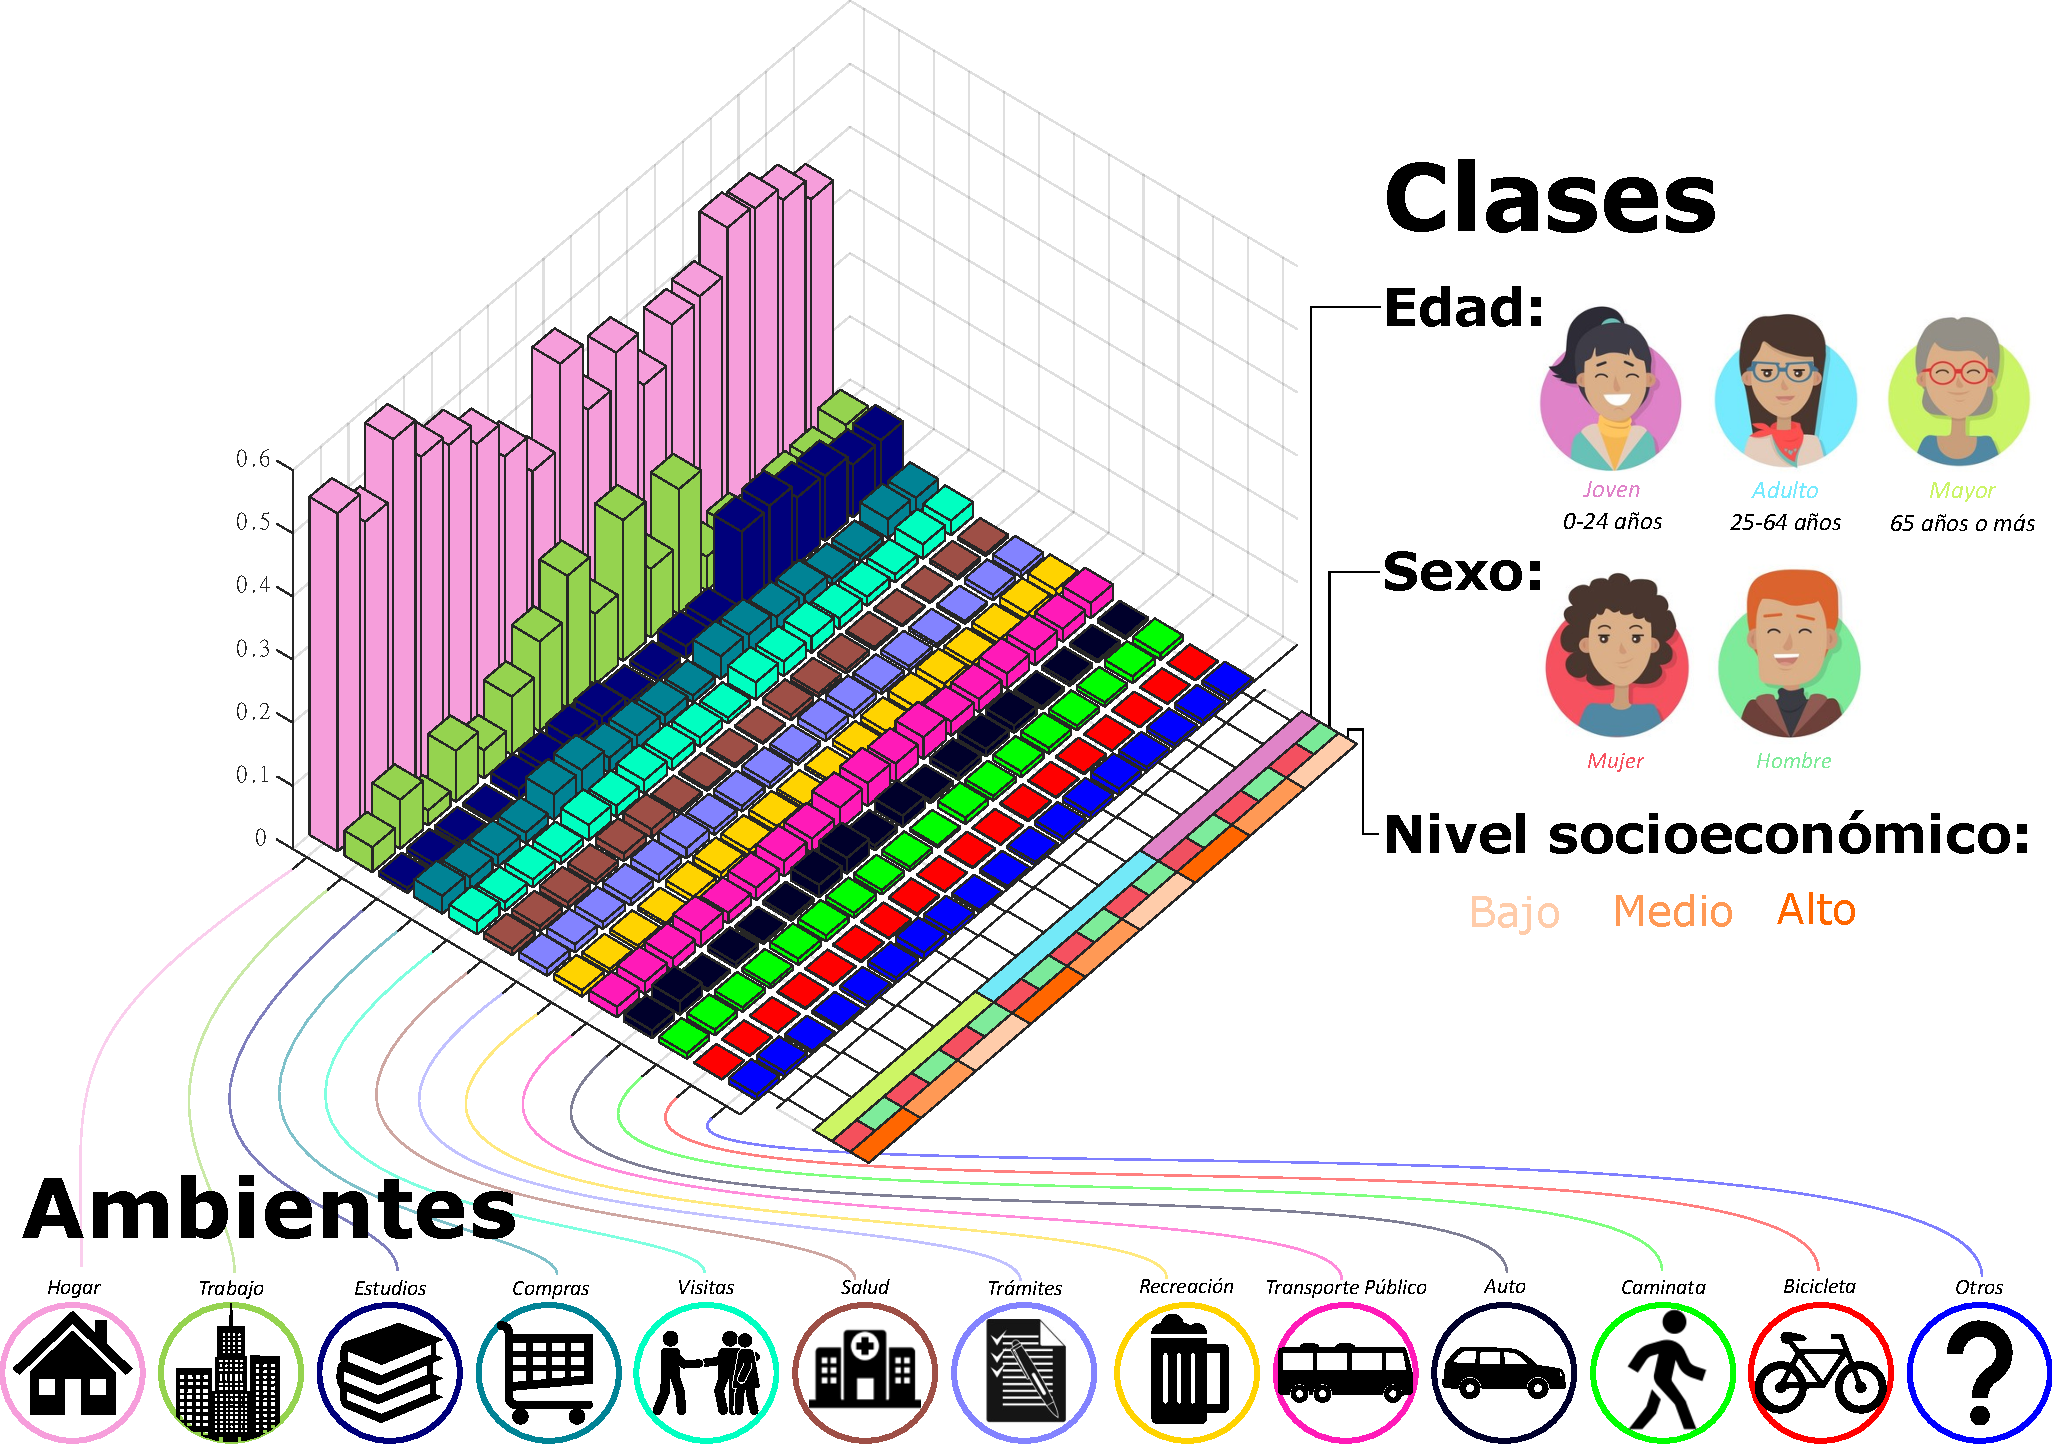
\includegraphics[width=0.99\textwidth]{img/resultados/matrixP/matriz Pambientesyclases.pdf}
\caption[Matriz detallada de tiempos de residencia para Santiago]{Matriz detallada de tiempos de residencia para Santiago. Considera clases basadas en nivel socioeconómico (según ingreso promedio del hogar), edad y sexo. 13 ambientes, basados en los propósitos de viajes de la encuesta. Se restan 7 horas del tiempo en el hogar (tiempo de sueño) y se normalizan las filas para que sumen 1.}
\label{img:Pmatrix-full}
\end{figure}

\subsubsection*{Matriz para las simulaciones}\label{res:matrix-normal-simulaciones}
%\noindent \textbf{Matriz para las simulaciones}

La aplicación del algoritmo tomando en consideración las decisiones tomadas en la sección \ref{subsec:eleccion-clases-ambientes}, específicamente la elección de 5 clases agrupadas por IPS como se detalla en la tabla \ref{table:ips-categ}, y del uso de los ambientes \texttt{hogar} y \texttt{exterior}. Se obtiene una matriz de tiempos de residencia \(P^0\) mucho más sencilla, presentada en la tabla \ref{table:matrix-simulaciones}.

\begin{table}[h!]
\centering
\begin{tabular}{||c c | c c ||} 
 \hline
 \textbf{Clase} & \textbf{Prioridad Social} &  \(P^0_{:,\text{hogar}}\) & \(P^0_{:,\text{exterior}}\)\\[1ex] 
 \hline
 1 & Sin Prioridad  & 0.73  & 0.27 \\ 
 2 & Baja           & 0.76  & 0.24 \\
 3 & Media Baja     & 0.77  & 0.23 \\
 4 & Media Alta     & 0.77  & 0.23 \\
 5 & Alta           & 0.77  & 0.23 \\ 
 \hline
\end{tabular}
\caption[Matriz de tiempos de residencia para las simulaciones.]{Matriz de tiempos de residencia para las simulaciones. La clase sin prioridad corresponde a la más acomodada y la clase con prioridad alta a la más vulnerable.}
\label{table:matrix-simulaciones}
\end{table}

\subsection{Santiago a lo largo del tiempo} \label{res:matrix-pandemia}

Una vez que una matriz \(P^0\) ha sido calculada, se requiere modificar esta matriz a fin de obtener \(P(t)\) que refleje el comportamiento de la población en pandemia. Estas modificaciones se hacen utilizando los datos de movilidad, siguiendo la metodología presentada en \ref{subsec:variaciones}; los datos de movilidad comunal son agregados ponderando por la población de la comuna, y suponiendo que la movilidad inicial era la misma en cada grupo.

La figura \ref{img:mov-pandemia} muestra la variación de movilidad para los distintos grupos socioeconómicos con respecto a la movilidad de la semana base. Se observa que la línea para la clase Sin Prioridad, es decir, la más acomodada, se mantiene por debajo de las otras, lo que significa que logró reducir su movilidad mucho más.

\begin{figure}[H]
\centering
\begin{subfigure}[b]{0.8\textwidth}
     \centering
     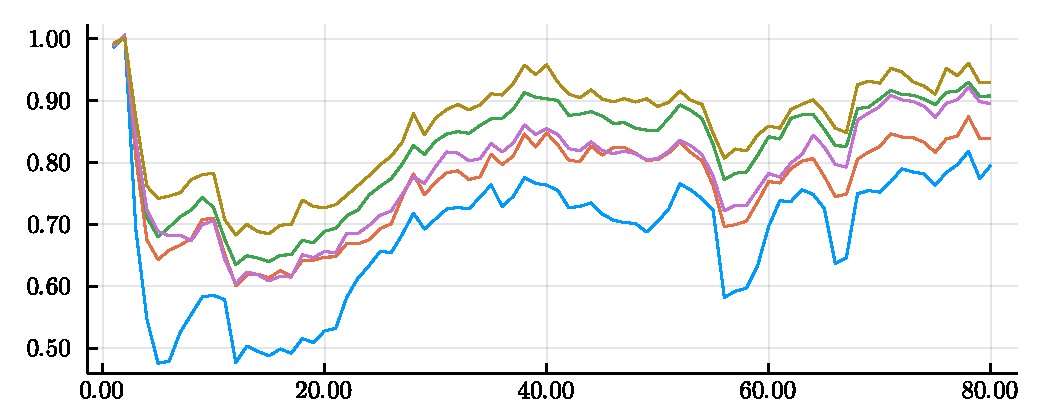
\includegraphics[width=0.99\textwidth]{img/resultados/mob-reduction.pdf}
\end{subfigure} 
\hfill
\begin{subfigure}[b]{0.99\textwidth}
 \centering
\scalebox{0.7}{
\begin{tikzpicture}
	\begin{pgfonlayer}{nodelayer}
		\node [style=none] (50) at (5, 0) {};
		\node [style=none] (51) at (7, 0) {};
		\node [style=none] (52) at (6, -0.5) {Prioridad Alta};
		\node [style=none] (53) at (2, 0) {};
		\node [style=none] (54) at (4, 0) {};
		\node [style=none] (55) at (3, -0.5) {Prioridad};
		\node [style=none] (56) at (-1, 0) {};
		\node [style=none] (57) at (1, 0) {};
		\node [style=none] (58) at (0, -0.5) {Prioridad};
		\node [style=none] (59) at (-4, 0) {};
		\node [style=none] (60) at (-2, 0) {};
		\node [style=none] (61) at (-3, -0.5) {Prioridad Baja};
		\node [style=none] (62) at (-7, 0) {};
		\node [style=none] (63) at (-5, 0) {};
		\node [style=none] (64) at (-6, -0.5) {Sin Prioridad};
		\node [style=none] (65) at (0, -1) {Media Baja};
		\node [style=none] (66) at (3, -1) {Media Alta};
	\end{pgfonlayer}
	\begin{pgfonlayer}{edgelayer}
		\draw [style=class5] (50.center) to (51.center);
		\draw [style=class1] (62.center) to (63.center);
		\draw [style=class2] (59.center) to (60.center);
		\draw [style=class3] (56.center) to (57.center);
		\draw [style=class4] (53.center) to (54.center);
	\end{pgfonlayer}
\end{tikzpicture}

}
\end{subfigure}
\caption[Fracción de la movilidad en pandemia por clase, c/r a movilidad normal.]{Fracción de la movilidad en pandemia por grupos, con respecto a la movilidad normal. Se considera la semana base como la correspondiente a 02/mar/2020 - 06/mar/2020.}
\label{img:mov-pandemia}
\end{figure}

 Ahora bien, al combinar esos datos con los de \ref{res:matrix-normal-simulaciones} se obtiene la imagen \ref{img:Pmatrix-pandemia-exterior}, que representa el tiempo de residencia estimado en el ambiente \texttt{exterior}. Se puede ver que, para la clases más acomodada, el mayor tiempo que pasan en el exterior compensa su mayor reducción de movilidad, haciendo menos notarias las diferencias.


\begin{figure}[!h]
\centering
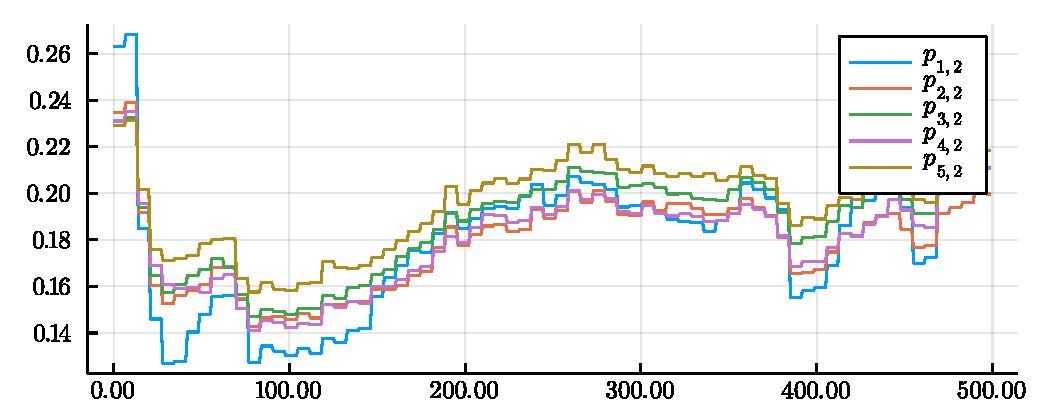
\includegraphics[width=0.8\textwidth]{img/resultados/tiempos-exterior.pdf}
\caption[Tiempo de residencia en \texttt{exterior} para las 5 clases elegidas.]{Tiempo de residencia en \texttt{exterior} para las 5 clases elegidas, desde 02/mar/2020.}
\label{img:Pmatrix-pandemia-exterior}
\end{figure}



\section{Análisis de sensibilidad}


\begin{figure}
\centering
\begin{tikzpicture}
	\begin{pgfonlayer}{nodelayer}
		\node [style=none] (0) at (-2, 2) {};
		\node [style=none] (1) at (0, 2) {};
		\node [style=none] (2) at (-2, 1) {};
		\node [style=none] (3) at (0, 1) {};
		\node [style=none] (4) at (-2, 0) {};
		\node [style=none] (5) at (0, 0) {};
		\node [style=none] (6) at (-2, -1) {};
		\node [style=none] (7) at (0, -1) {};
		\node [style=none] (8) at (2, 2) {$0.15$};
		\node [style=none] (9) at (2, 1) {};
		\node [style=none] (10) at (2, 1) {};
		\node [style=none] (11) at (2, 1) {$0.25$};
		\node [style=none] (12) at (2, 0) {};
		\node [style=none] (13) at (2, 0) {$0.35$};
		\node [style=none] (14) at (2, -1) {};
		\node [style=none] (15) at (2, -1) {$0.45$};
		\node [style=none] (16) at (0, 3) {};
		\node [style=none] (17) at (0, 3) {Condición inicial $\alpha_0$};
		\node [style=none] (18) at (6, 3) {};
		\node [style=none] (19) at (6, 3) {$\beta_{\textrm{ext}}$};
		\node [style=none] (20) at (0, -3) {};
		\node [style=none] (21) at (0, -3) {Solución real};
		\node [style=none] (22) at (-2, -4) {};
		\node [style=none] (23) at (0, -4) {};
		\node [style=none] (24) at (2, -4) {};
		\node [style=none] (25) at (2, -4) {$1.88$};
		\node [style=none] (26) at (4, 2) {};
		\node [style=none] (27) at (6, 2) {};
		\node [style=none] (28) at (4, 1) {};
		\node [style=none] (29) at (6, 1) {};
		\node [style=none] (30) at (4, 0) {};
		\node [style=none] (31) at (6, 0) {};
		\node [style=none] (32) at (4, -1) {};
		\node [style=none] (33) at (6, -1) {};
		\node [style=none] (34) at (4, -2) {};
		\node [style=none] (35) at (6, -2) {};
		\node [style=none] (36) at (4, -3) {};
		\node [style=none] (37) at (6, -3) {};
		\node [style=none] (38) at (4, -4) {};
		\node [style=none] (39) at (6, -4) {};
		\node [style=none] (40) at (4, -5) {};
		\node [style=none] (41) at (6, -5) {};
		\node [style=none] (42) at (8, 2) {$1.2$};
		\node [style=none] (43) at (8, 1) {$1.5$};
		\node [style=none] (44) at (8, 0) {$1.8$};
		\node [style=none] (45) at (8, -1) {$2.1$};
		\node [style=none] (46) at (8, -2) {$2.4$};
		\node [style=none] (47) at (8, -3) {$2.7$};
		\node [style=none] (48) at (8, -4) {$3.0$};
		\node [style=none] (49) at (8, -5) {$3.3$};
	\end{pgfonlayer}
	\begin{pgfonlayer}{edgelayer}
		\draw [style={a0_1}] (0.center) to (1.center);
		\draw [style={a0_2}] (2.center) to (3.center);
		\draw [style={a0_3}] (4.center) to (5.center);
		\draw [style={a0_4}] (6.center) to (7.center);
		\draw [style=real] (22.center) to (23.center);
		\draw [style=beta1] (26.center) to (27.center);
		\draw [style=beta2] (28.center) to (29.center);
		\draw [style=beta3] (30.center) to (31.center);
		\draw [style=beta4] (32.center) to (33.center);
		\draw [style=beta5] (34.center) to (35.center);
		\draw [style=beta6] (36.center) to (37.center);
		\draw [style=beta7] (38.center) to (39.center);
		\draw [style=beta8] (40.center) to (41.center);
	\end{pgfonlayer}
\end{tikzpicture}

\caption{Leyenda sensibilidad ante \(\beta_{\text{exterior}}\).} \label{fig:legend-sensi-b}
\end{figure}



% Resultados de usar el filtro de kalman 
\section{Estimación de parámetros}\label{sec:estimacion-results}

En todos los resultados presentados se utiliza \(\Delta t = 1 \text{día}\). Se probó con valores más pequeños sin alterar el desempeño del método.

%\subsection{Modelo con una clase}
\subsection{Modelo multiclase con datos sintéticos} \label{subsec:sintetico}

Se utilizan los datos de movilidad de dos comunas (San Bernardo y las Condes) para generar las matrices de tiempos de residencia variables en el tiempo. Se fijan valores \(\gamma_E = 1/5.1, \gamma_I = 1/8.2\) y condiciones iniciales... Se fija riesgos \(\beta_{\text{hogar}} = 1\) y \(\beta_{\text{exterior}} = 1.88\). 

Mediante prueba y error se genera dos controles diferentes para cada clase, de forma que el total de casos acumulados tengan órdenes de magnitud similares a los datos reales.

A partir de la solución de la ecuación diferencial es posible obtener las series \(C_1, C_2\). Las observaciones son obtenidas con \(\Delta t = 1\) [día]. Se utilizan estas observaciones directamente (sin añadir ruido), y el filtro asume que tienen un ruido pequeño (G = diag(10)...). 

Se suponen condiciones iniciales diferentes a las utilizadas en la solución (...), y se eligen matrices de covarianza de tal forma de obtener resultados razonables. Un ejemplo de las estimaciones de estado obtenidas puede verse en la figura \ref{synth-all-nohigh}.



\begin{figure}[!h]
\centering
\includegraphics[width=0.99\textwidth]{img/resultados/synth/kalman_grouped_allstates_allgroups\parameterstring}
\caption{Ejemplo de estimación de estados y parámetros variables en el tiempo con \textit{Kalman Smoother}, a partir de las observaciones del número de casos acumulados \(C_1, C_2\).}
\label{synth-all-nohigh}
\end{figure}

Las matrices de covarianza iniciales son elegidas de modo tal que las soluciones reales quedan a una desviación estándar de la estimación, como se ve en la figura \ref{synth-e-comp-high}.


\begin{figure}[!h]
     \centering
     \begin{subfigure}[b]{\textwidth}
         \centering
         \includegraphics[width=.8\textwidth]{img/resultados/synth/kalman_grouped_E_high1\parameterstring}
         \caption{Clase \(1\).}
     \end{subfigure}
     \hfill
     \begin{subfigure}[b]{\textwidth}
         \centering
         \includegraphics[width=0.8\textwidth]{img/resultados/synth/kalman_grouped_E_high2\parameterstring}
         \caption{Clase \(2\).}
     \end{subfigure}
        \caption{Casos Expuestos, comparando resultados obtenidos con solución real, en valores absolutos y normalizados con respecto a la cantidad de personas por clase.}
        \label{synth-e-comp-high}
\end{figure}


Como se ve en la figura \ref{synth-alpha-comp-high}, es posible estimar el factor sanitario a partir de los datos, con ciertas consideraciones. En las secciones siguientes  se hablará en más detalle de la sensibilidad de la estimación con respecto a los parámetros del filtro. Más específicamente, se estudia la sensibilidad de la estimación del factor sanitario con respecto al parámetro \(\beta_{\text{exterior}}\) y la condición inicial. Se recuerda que se hizo la simplificación de que los ruidos en la dinámica son independientes, es decir que el ruido está dado por una matriz normal multivariada con matriz de covarianzas diagonal. Nos interesa por tanto, solo la diagonal de la matriz, las varianzas. Se muestra el efecto en la estimación al usar distintos valores para la matriz de varianzas.

\begin{figure}[!h]
     \centering
     \begin{subfigure}[b]{\textwidth}
         \centering
         \includegraphics[width=.99\textwidth]{img/resultados/synth/kalman_grouped_alpha_high1\parameterstring}
         \caption{Clase \(1\).}
     \end{subfigure}
     \hfill
     \begin{subfigure}[b]{\textwidth}
         \centering
         \includegraphics[width=0.99\textwidth]{img/resultados/synth/kalman_grouped_alpha_high2\parameterstring}
         \caption{Clase \(2\).}
     \end{subfigure}
        \caption[Factor sanitario, caso sintético]{Factor sanitario, comparando resultados obtenidos con función de control usada para general los datos, acotando el dominio en el eje \(y\) para mejor apreciación.}
        \label{synth-alpha-comp-high}
\end{figure}


\subsection{Sensibilidad con respecto a \(\beta_{\text{exterior}}\) y \(\alpha_0\)} \label{subsec:sensibeta}

\begin{figure}[H]
\centering
\begin{subfigure}[b]{0.47\textwidth}
     \centering
     \includegraphics[width=\textwidth]{img/resultados/synth/\stringsensiparam_high1_\stringrealandcovsparam\stringparamtwo.pdf}
     \caption{Estimación control clase 1, suponiendo conocidos \(\gamma_E = 1/5.1\) y \(\gamma_I = 1/7.2\)}
     \label{fig:legend-sensi-b-class1-gamma_real}
\end{subfigure} 
\hfill
\begin{subfigure}[b]{0.47\textwidth}
     \centering
     \includegraphics[width=\textwidth]{img/resultados/synth/\stringsensiparam_high2_\stringrealandcovsparam\stringparamtwo.pdf}
     \caption{Estimación control clase 2,  suponiendo conocidos \(\gamma_E = 1/5.1\) y \(\gamma_I = 1/7.2\)}
     \label{fig:legend-sensi-b-class2-gamma_real}
\end{subfigure} 
\hfill
\begin{subfigure}[b]{0.47\textwidth}
     \centering
     \includegraphics[width=\textwidth]{img/resultados/synth/\stringsensiparam_high1_\stringrealandcovsparam\stringparamthree.pdf}
     \caption{Estimación control clase 1,  con \(\gamma_E = 1/5.8\) y \(\gamma_I = 1/8.2\)}
     \label{fig:legend-sensi-b-class1-gamma_estimado}
\end{subfigure} 
\hfill
\begin{subfigure}[b]{0.47\textwidth}
     \centering
     \includegraphics[width=\textwidth]{img/resultados/synth/\stringsensiparam_high2_\stringrealandcovsparam\stringparamthree.pdf}
     \caption{Estimación control clase 2,  con \(\gamma_E = 1/5.8\) y \(\gamma_I = 1/8.2\)}
     \label{fig:legend-sensi-b-class2-gamma_estimado}
\end{subfigure} 
\hfill
\begin{subfigure}[b]{0.75\textwidth}
 \centering
\scalebox{0.7}{
\begin{tikzpicture}
	\begin{pgfonlayer}{nodelayer}
		\node [style=none] (0) at (-0.5, 1.25) {};
		\node [style=none] (1) at (1, 1.25) {};
		\node [style=none] (2) at (-0.5, 0.75) {};
		\node [style=none] (3) at (1, 0.75) {};
		\node [style=none] (4) at (-0.5, 0.25) {};
		\node [style=none] (5) at (1, 0.25) {};
		\node [style=none] (6) at (-0.5, -0.25) {};
		\node [style=none] (7) at (1, -0.25) {};
		\node [style=none] (8) at (1.5, 1.25) {$0.15$};
		\node [style=none] (9) at (1.5, 0.75) {};
		\node [style=none] (10) at (1.5, 0.75) {};
		\node [style=none] (11) at (1.5, 0.75) {$0.25$};
		\node [style=none] (12) at (1.5, 0.25) {};
		\node [style=none] (13) at (1.5, 0.25) {$0.35$};
		\node [style=none] (15) at (1.5, -0.25) {$0.45$};
		\node [style=none] (17) at (0.5, 1.75) {Condición inicial $\alpha_0$};
		\node [style=none] (19) at (12.5, 2.5) {$\beta_{\textrm{ext}}$};
		\node [style=none] (21) at (6.5, 1) {$\beta_{\text{ext}}$ solución real};
		\node [style=none] (22) at (5.5, 0.5) {};
		\node [style=none] (23) at (7, 0.5) {};
		\node [style=none] (24) at (7.5, 0.5) {};
		\node [style=none] (25) at (7.5, 0.5) {$1.88$};
		\node [style=none] (26) at (11.5, 2) {};
		\node [style=none] (27) at (13, 2) {};
		\node [style=none] (28) at (11.5, 1.5) {};
		\node [style=none] (29) at (13, 1.5) {};
		\node [style=none] (30) at (11.5, 1) {};
		\node [style=none] (31) at (13, 1) {};
		\node [style=none] (32) at (11.5, 0.5) {};
		\node [style=none] (33) at (13, 0.5) {};
		\node [style=none] (34) at (11.5, 0) {};
		\node [style=none] (35) at (13, 0) {};
		\node [style=none] (36) at (11.5, -0.5) {};
		\node [style=none] (37) at (13, -0.5) {};
		\node [style=none] (38) at (11.5, -1) {};
		\node [style=none] (39) at (13, -1) {};
		\node [style=none] (40) at (11.5, -1.5) {};
		\node [style=none] (41) at (13, -1.5) {};
		\node [style=none] (42) at (13.5, 2) {$1.2$};
		\node [style=none] (43) at (13.5, 1.5) {$1.5$};
		\node [style=none] (44) at (13.5, 1) {$1.8$};
		\node [style=none] (45) at (13.5, 0.5) {$2.1$};
		\node [style=none] (46) at (13.5, 0) {$2.4$};
		\node [style=none] (47) at (13.5, -0.5) {$2.7$};
		\node [style=none] (48) at (13.5, -1) {$3.0$};
		\node [style=none] (49) at (13.5, -1.5) {$3.3$};
	\end{pgfonlayer}
	\begin{pgfonlayer}{edgelayer}
		\draw [style={a0_1}] (0.center) to (1.center);
		\draw [style={a0_2}] (2.center) to (3.center);
		\draw [style={a0_3}] (4.center) to (5.center);
		\draw [style={a0_4}] (6.center) to (7.center);
		\draw [style=real] (22.center) to (23.center);
		\draw [style=beta1] (26.center) to (27.center);
		\draw [style=beta2] (28.center) to (29.center);
		\draw [style=beta3] (30.center) to (31.center);
		\draw [style=beta4] (32.center) to (33.center);
		\draw [style=beta5] (34.center) to (35.center);
		\draw [style=beta6] (36.center) to (37.center);
		\draw [style=beta7] (38.center) to (39.center);
		\draw [style=beta8] (40.center) to (41.center);
	\end{pgfonlayer}
\end{tikzpicture}
}
\end{subfigure}

\caption[Sensibilidad ante riesgo exterior y condición inicial del factor sanitario.]{Sensibilidad ante riesgo exterior y condición inicial del factor sanitario. Cada color representa un condición inicial diferente usada en la estimación, mientras que la opacidad de la solución representa la distancia de \(\beta_{\text{exterior}}\) al valor real; a mayor transparencia, más lejano.} \label{fig:legend-sensi-b}
\end{figure}

Los riesgos \(\beta \), las tasas \(\gamma_E\) y \(\gamma_I\), así como las condiciones iniciales, serán valores desconocidos en la práctica. Esta sección estudia el efecto de estos valores en la solución estimada. 

% gamma_e_real = 1/5.1; gamma_i_real = 1/7.2; beta_exterior_real = 1.88; 
Utilizando el caso sintético ya presentado, se estudia el efecto del valor \(\beta_{\text{exterior}}\) y de las condiciones iniciales para factor sanitario \(\alpha\) en los resultados. Los datos de casos acumulados observados fueron generados con un control conocido (línea verde) y parámetros \(\gamma_E = 1/5.1 [\text{días}]^{-1}\), \(\gamma_I = 1/7.2 [\text{días}]^{-1}\) y \(\beta_{\text{exterior}} = 1.88\).

Para distintos valores de \(\beta_{\text{exterior}}\) y distintas condiciones iniciales para el factor sanitario, se estima el factor sanitario suavizado a lo largo del tiempo y se compara con el valor de control usado para generar los datos. Los resultados pueden verse en la figura \ref{fig:legend-sensi-b}. Se estudian dos casos; uno con tasas de incubación \(\gamma_E\) y de remoción \(\gamma_I\) son conocidos (figuras \ref{fig:legend-sensi-b-class1-gamma_real} y \ref{fig:legend-sensi-b-class2-gamma_real}) y otro donde se utilizan valores pausibles para ambos parámetros (figuras \ref{fig:legend-sensi-b-class1-gamma_estimado} y \ref{fig:legend-sensi-b-class2-gamma_estimado}).

Se observa que tras una cierta cantidad de tiempo (\(t \geq 50\) la condición inicial es irrelevante y todas las soluciones dadas por un mismo \(\beta_{\text{exterior}}\) siguen la misma trayectoria. Al comenzar en una condición inicial demasiado baja, como \(\alpha_0 = 0.15\), se observa una tendencia a sobrecorregir el error antes de llegar a la trayectoria común. 

Para \(t \geq 200\), la estimación es menos exacta. Esto ya era visible en la figura \ref{synth-alpha-comp-high}, y probablemente se debe al hecho de que en este caso particular, para ese tiempo \(S_i(t) \approx 0\), así que la solución ya no es sensible al parámetro \(\alpha_i\).

Cuando los parámetros \(\gamma_E\) y \(\gamma_I\) son conocidos, la estimación del factor sanitario es más certera al usar un valor \(\beta_{\text{exterior}}\) más cercano al real. Esto se observa en la figuras \ref{fig:legend-sensi-b-class1-gamma_real} y \ref{fig:legend-sensi-b-class2-gamma_real}, donde las estimaciones más oscuras están justo en la línea verde que marca el factor sanitario de control usado para generar los datos.

En el caso en que los parámetros \(\gamma_E\) y \(\gamma_I\) son desconocidos y solo se usan valores pausibles, la estimación es menos exacata; el factor sanitario (para este caso particular) es subestimado al usar \(\beta_{\text{exterior}} = 1.8\), el más cercano al real (\(1.88\)) de entre los utilizados. Esto se observa en la figuras \ref{fig:legend-sensi-b-class1-gamma_estimado} y \ref{fig:legend-sensi-b-class2-gamma_estimado}, donde las estimaciones más oscuras están por debajo de la línea verde del factor sanitario de control.

%gamma_e_real = 1/5.1; gamma_i_real = 1/7.2; beta_exterior_real = 1.88; 

%gamma_e = 1/5.8 ; gamma_i = 1/8.2; beta_exterior = 2.



\subsection{Sensibilidad ante los parámetros \(\gamma_E, \gamma_I\)} \label{subsec:sensigamma}

\subsection{Sensibilidad ante la covarianza} \label{subsec:sensicov}
% 20. .^ collect(-2:0.4:0)
\begin{figure}[H]
\centering
\begin{subfigure}[b]{0.47\textwidth}
     \centering
     %\includegraphics[width=\textwidth]{img/resultados/synth/sensialphacov_alphacov0-003\stringsensiacov\stringparamfour.pdf}
     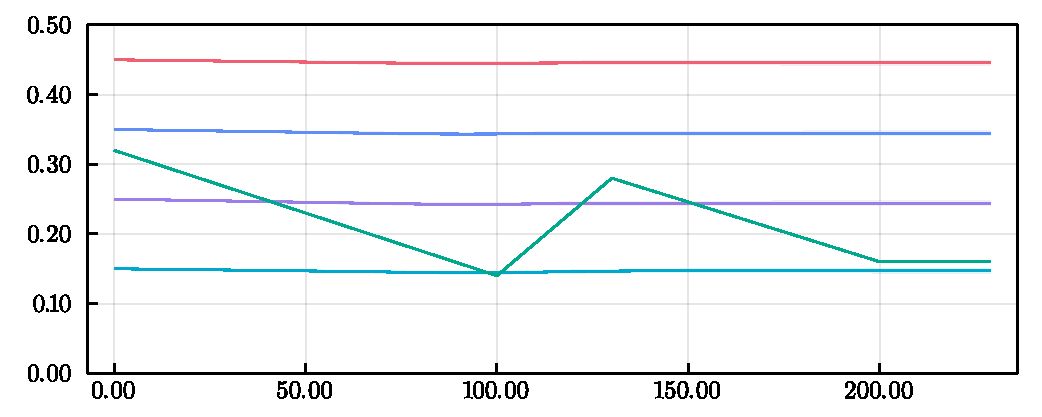
\includegraphics[width=\textwidth]{img/resultados/synth/sensialphacov_alphacov0-003_0alphaini0-15_0-1_0-45_high1_b2real1-88_gereal0-1961_gireal0-1389_acov0-8_aini0-27675_gcov0-05gamma_e_0-1961_gamma_i_0-1389_beta_2_1-8800.pdf}
     \caption{Estimación control clase 1, usando varianza para \(\alpha\) \(20^{-2.0}\)}
     \label{fig:legend-sensi-acov-class1--a}
\end{subfigure} 
\hfill
\begin{subfigure}[b]{0.47\textwidth}
     \centering
     %\includegraphics[width=\textwidth]{img/resultados/synth/sensialphacov_alphacov0-008\stringsensiacov\stringparamfour.pdf}
     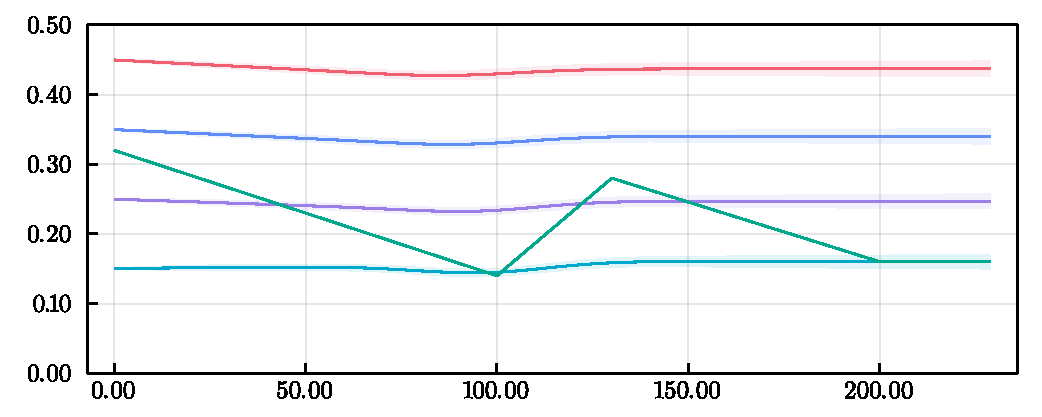
\includegraphics[width=\textwidth]{img/resultados/synth/sensialphacov_alphacov0-008_0alphaini0-15_0-1_0-45_high1_b2real1-88_gereal0-1961_gireal0-1389_acov0-8_aini0-27675_gcov0-05gamma_e_0-1961_gamma_i_0-1389_beta_2_1-8800.pdf}
     \caption{Estimación control clase 1, usando varianza para \(\alpha\) \(20^{-1.6}\)}
     \label{fig:legend-sensi-acov-class1--b}
\end{subfigure} 
\hfill
\begin{subfigure}[b]{0.47\textwidth}
     \centering
     %\includegraphics[width=\textwidth]{img/resultados/synth/sensialphacov_alphacov0-027\stringsensiacov\stringparamfour.pdf}
     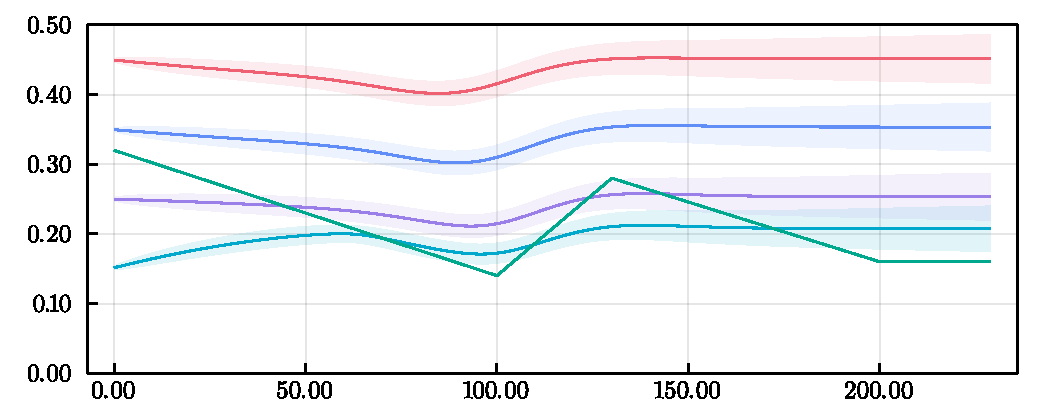
\includegraphics[width=\textwidth]{img/resultados/synth/sensialphacov_alphacov0-027_0alphaini0-15_0-1_0-45_high1_b2real1-88_gereal0-1961_gireal0-1389_acov0-8_aini0-27675_gcov0-05gamma_e_0-1961_gamma_i_0-1389_beta_2_1-8800.pdf}
     \caption{Estimación control clase 1, usando varianza para \(\alpha\) \(20^{-1.2}\)}
     \label{fig:legend-sensi-acov-class1--c}
\end{subfigure} 
\hfill
\begin{subfigure}[b]{0.47\textwidth}
     \centering
     %\includegraphics[width=\textwidth]{img/resultados/synth/sensialphacov_alphacov0-091\stringsensiacov\stringparamfour.pdf}
     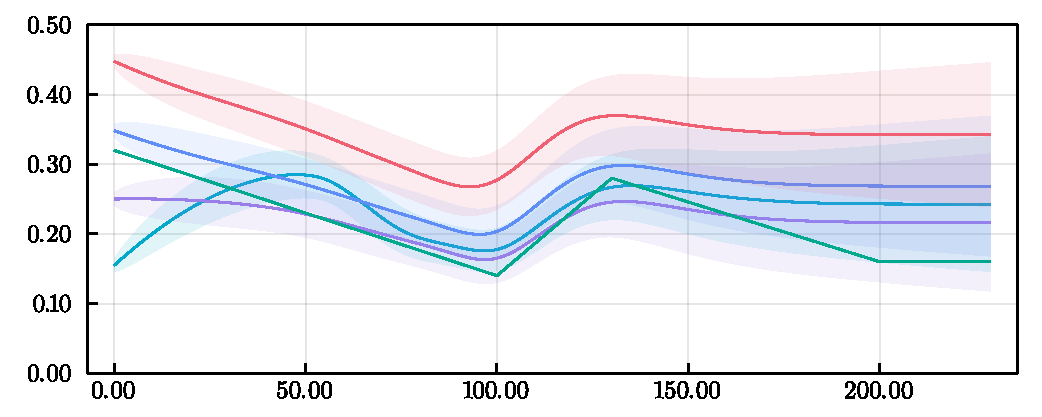
\includegraphics[width=\textwidth]{img/resultados/synth/sensialphacov_alphacov0-091_0alphaini0-15_0-1_0-45_high1_b2real1-88_gereal0-1961_gireal0-1389_acov0-8_aini0-27675_gcov0-05gamma_e_0-1961_gamma_i_0-1389_beta_2_1-8800.pdf}
     \caption{Estimación control clase 1, usando varianza para \(\alpha\) \(20^{-0.8}\)}
     \label{fig:legend-sensi-acov-class1--d}
\end{subfigure} 
\hfill
\begin{subfigure}[b]{0.47\textwidth}
     \centering
     %\includegraphics[width=\textwidth]{img/resultados/synth/sensialphacov_alphacov0-302\stringsensiacov\stringparamfour.pdf}
     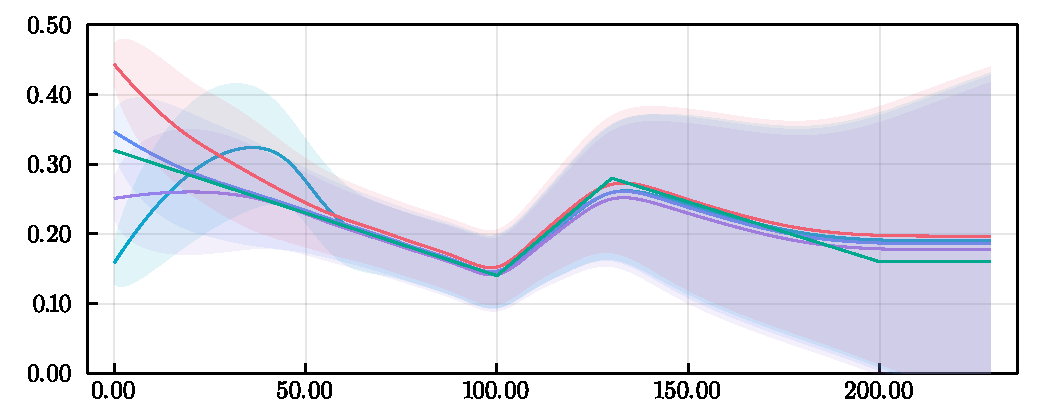
\includegraphics[width=\textwidth]{img/resultados/synth/sensialphacov_alphacov0-302_0alphaini0-15_0-1_0-45_high1_b2real1-88_gereal0-1961_gireal0-1389_acov0-8_aini0-27675_gcov0-05gamma_e_0-1961_gamma_i_0-1389_beta_2_1-8800.pdf}
     \caption{Estimación control clase 1, usando varianza para \(\alpha\) \(20^{-0.4}\)}
     \label{fig:legend-sensi-acov-class1--e}
\end{subfigure} 
\hfill
\begin{subfigure}[b]{0.47\textwidth}
     \centering
     %\includegraphics[width=\textwidth]{img/resultados/synth/sensialphacov_alphacov1-000\stringsensiacov\stringparamfour.pdf}
     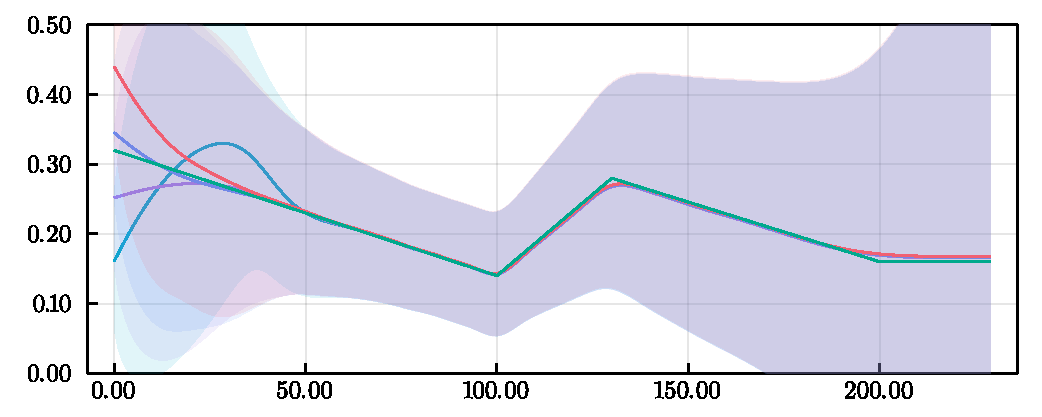
\includegraphics[width=\textwidth]{img/resultados/synth/sensialphacov_alphacov1-000_0alphaini0-15_0-1_0-45_high1_b2real1-88_gereal0-1961_gireal0-1389_acov0-8_aini0-27675_gcov0-05gamma_e_0-1961_gamma_i_0-1389_beta_2_1-8800.pdf}
     \caption{Estimación control clase 1, usando varianza para \(\alpha\) \(20^{0.0}\)}
     \label{fig:legend-sensi-acov-class1--f}
\end{subfigure} 
\hfill
\begin{subfigure}[b]{0.75\textwidth}
 \centering
\scalebox{0.7}{
\begin{tikzpicture}
	\begin{pgfonlayer}{nodelayer}
		\node [style=none] (0) at (-0.5, 1.25) {};
		\node [style=none] (1) at (1, 1.25) {};
		\node [style=none] (2) at (-0.5, 0.75) {};
		\node [style=none] (3) at (1, 0.75) {};
		\node [style=none] (4) at (-0.5, 0.25) {};
		\node [style=none] (5) at (1, 0.25) {};
		\node [style=none] (6) at (-0.5, -0.25) {};
		\node [style=none] (7) at (1, -0.25) {};
		\node [style=none] (8) at (1.5, 1.25) {$0.15$};
		\node [style=none] (9) at (1.5, 0.75) {};
		\node [style=none] (10) at (1.5, 0.75) {};
		\node [style=none] (11) at (1.5, 0.75) {$0.25$};
		\node [style=none] (12) at (1.5, 0.25) {};
		\node [style=none] (13) at (1.5, 0.25) {$0.35$};
		\node [style=none] (15) at (1.5, -0.25) {$0.45$};
		\node [style=none] (17) at (0.5, 1.75) {Condición inicial $\alpha_0$};
		\node [style=none] (21) at (6.5, 1) {};
		\node [style=none] (22) at (5.5, 0.5) {};
		\node [style=none] (23) at (7, 0.5) {};
		\node [style=none] (24) at (7.5, 0.5) {};
		\node [style=none] (25) at (7.5, 0.5) {Solución real};
	\end{pgfonlayer}
	\begin{pgfonlayer}{edgelayer}
		\draw [style={a0_1}] (0.center) to (1.center);
		\draw [style={a0_2}] (2.center) to (3.center);
		\draw [style={a0_3}] (4.center) to (5.center);
		\draw [style={a0_4}] (6.center) to (7.center);
		\draw [style=real] (22.center) to (23.center);
	\end{pgfonlayer}
\end{tikzpicture}
}
\end{subfigure}
\caption[Sensibilidad ante la varianza y condición inicial del factor sanitario.]{Sensibilidad ante la varianza y condición inicial del factor sanitario. Cada color representa una condición inicial diferente usada en la estimación.} \label{fig:legend-sensi-alphacov}
\end{figure}

Se recuerda que se hizo la simplificación de que los ruidos en la dinámica son independientes, es decir que el ruido está dado por una matriz normal multivariada con matriz de covarianzas diagonal. Nos interesa por tanto, solo la diagonal de la matriz, las varianzas. Se muestra el efecto en la estimación al usar distintos valores para la matriz de varianzas.

La figura \ref{fig:legend-sensi-alphacov} muestra la estimación del factor sanitario para distintos valores de varianza del ruido en la dinámica de este. Este valor refleja la certeza que tenemos en la dinámica del estado; si hay mucha, se usa una varianza baja. Si no hay tanta seguridad, se usa una varianza mayor, de tal forma de incorporar la información de los datos. Los gráficos  \ref{fig:legend-sensi-acov-class1--a} y \ref{fig:legend-sensi-acov-class1--b}  muestran lo que ocurre al utilizar una varianza demasiado baja en el estado aumentado; la estimación es muy insensible a los datos, y se queda muy cercana a la condición inicial dada. Tanto en \ref{fig:legend-sensi-acov-class1--c} como en \ref{fig:legend-sensi-acov-class1--d} ya va siendo posible percibir variaciones en el control, pero aún no se ve convergencia desde las distintas condiciones iniciales. Finalmente, los gráficos  \ref{fig:legend-sensi-acov-class1--e} y \ref{fig:legend-sensi-acov-class1--f} tienen suficiente varianza, como se ve en la convergencia de las estimaciones a partir de \(t >=50\) aproximadamente, sin embargo \ref{fig:legend-sensi-acov-class1--f} usa una varianza excesiva, ya que pueden obtenerse resultados similares con una mayor certeza.



%\subsection{Efecto del \textit{smoother}}\label{subsec:smoother}

\subsection{Modelo con datos reales}\label{subsec:datosreales}

El estudio realizado en las subsecciones anteriores entrega herramientas para trabajar con el caso real.



\begin{table}[h!]
\centering
\begin{tabular}{|| m{1cm} m{3cm} m{8cm}||} 
 \hline
 & \textbf{Fecha} & \textbf{Evento} \\
 \hline 
 (1) & 13/may/2020 & Comienzo de la cuarentena total en la RM.\\
 (2) & 28/jul/2020 & Comienza a regir el Plan Paso a Paso.\\
 (3) & 04/ene/2021 & Comienza a funcionar el pase de vacaciones.\\ 
 (4) & 03/feb/2021 & Comienza campaña de vacunación masiva (ver \ref{}).\\
 (5) & 26/may/2021 &  Un 50\% de la población en la RM tiene la primera dosis de la vacuna. \\
 \hline
\end{tabular}
\caption{Algunas fechas relevantes para el desarrollo de la pandemia en Santiago.}
\label{table:fechas-relevantes}
\end{table}


\begin{figure}[H]
\centering
\includegraphics[width=0.99\textwidth]{img/resultados/kalman_grouped_allstates_allgroups\parameterstring}
\caption[\textit{Kalman RTS Smoother} aplicado al caso real ]{\textit{Kalman RTS Smoother} aplicado al caso real. Se utiliza el Producto 15 de casos acumulados confirmados}
\label{all-nohigh}
\end{figure}



\begin{figure}[H]
     \centering
     \begin{subfigure}[b]{0.47\textwidth}
         \centering
         \includegraphics[width=\textwidth]{img/resultados/kalman_grouped_I_high1\parameterstring}
         \caption{Clase \(1\).}
     \end{subfigure}
     \hfill
     \begin{subfigure}[b]{.47\textwidth}
         \centering
         \includegraphics[width=\textwidth]{img/resultados/kalman_grouped_I_high2\parameterstring}
         \caption{Clase \(2\).}
     \end{subfigure}
     \hfill
     \begin{subfigure}[b]{.47\textwidth}
         \centering
         \includegraphics[width=\textwidth]{img/resultados/kalman_grouped_I_high3\parameterstring}
         \caption{Clase \(3\).}
     \end{subfigure}
     \hfill
     \begin{subfigure}[b]{.47\textwidth}
         \centering
         \includegraphics[width=\textwidth]{img/resultados/kalman_grouped_I_high4\parameterstring}
         \caption{Clase \(4\).}
     \end{subfigure}
     \hfill
     \begin{subfigure}[b]{.47\textwidth}
         \centering
         \includegraphics[width=\textwidth]{img/resultados/kalman_grouped_I_high5\parameterstring}
         \caption{Clase \(5\).}
     \end{subfigure}
     \hfill
     \begin{subfigure}[b]{.47\textwidth}
         \centering
         \includegraphics[width=\textwidth]{img/resultados/kalman_grouped_I_allclass\parameterstring}
         \caption{Todas las clases.}
     \end{subfigure}
        \caption{Cantidad de Infectados estimados a partir de datos reales, en valores absolutos y normalizados con respecto a la cantidad de personas por clase.}
        \label{e-comp-high}
\end{figure}



\begin{figure}[H]
     \centering
     \begin{subfigure}[b]{0.47\textwidth}
         \centering
         \includegraphics[width=\textwidth]{img/resultados/kalman_grouped_S_high1\parameterstring}
         \caption{Clase \(1\).}
     \end{subfigure}
     \hfill
     \begin{subfigure}[b]{.47\textwidth}
         \centering
         \includegraphics[width=\textwidth]{img/resultados/kalman_grouped_S_high2\parameterstring}
         \caption{Clase \(2\).}
     \end{subfigure}
     \hfill
     \begin{subfigure}[b]{.47\textwidth}
         \centering
         \includegraphics[width=\textwidth]{img/resultados/kalman_grouped_S_high3\parameterstring}
         \caption{Clase \(3\).}
     \end{subfigure}
     \hfill
     \begin{subfigure}[b]{.47\textwidth}
         \centering
         \includegraphics[width=\textwidth]{img/resultados/kalman_grouped_S_high4\parameterstring}
         \caption{Clase \(4\).}
     \end{subfigure}
     \hfill
     \begin{subfigure}[b]{.47\textwidth}
         \centering
         \includegraphics[width=\textwidth]{img/resultados/kalman_grouped_S_high5\parameterstring}
         \caption{Clase \(5\).}
     \end{subfigure}
     \hfill
     \begin{subfigure}[b]{.47\textwidth}
         \centering
         \includegraphics[width=\textwidth]{img/resultados/kalman_grouped_S_allclass\parameterstring}
         \caption{Todas las clases.}
     \end{subfigure}
        \caption{Cantidad de Susceptibles estimados a partir de datos reales, en valores absolutos y normalizados con respecto a la cantidad de personas por clase.}
        \label{s-comp-high}
\end{figure}




\begin{figure}[H]
     \centering
     \begin{subfigure}[b]{.99\textwidth}
         \centering
         \includegraphics[width=\textwidth]{img/resultados/kalman_grouped_alpha_allclass\parameterstring}
         \caption{Todas las clases.}
     \end{subfigure}
     \hfill
     \begin{subfigure}[b]{0.47\textwidth}
         \centering
         \includegraphics[width=\textwidth]{img/resultados/kalman_grouped_alpha_high1\parameterstring}
         \caption{Clase \(1\).}
     \end{subfigure}
     \hfill
     \begin{subfigure}[b]{.47\textwidth}
         \centering
         \includegraphics[width=\textwidth]{img/resultados/kalman_grouped_alpha_high2\parameterstring}
         \caption{Clase \(2\).}
     \end{subfigure}
     \hfill
     \begin{subfigure}[b]{.47\textwidth}
         \centering
         \includegraphics[width=\textwidth]{img/resultados/kalman_grouped_alpha_high3\parameterstring}
         \caption{Clase \(3\).}
     \end{subfigure}
     \hfill
     \begin{subfigure}[b]{.47\textwidth}
         \centering
         \includegraphics[width=\textwidth]{img/resultados/kalman_grouped_alpha_high4\parameterstring}
         \caption{Clase \(4\).}
     \end{subfigure}
     \hfill
     \begin{subfigure}[b]{.47\textwidth}
         \centering
         \includegraphics[width=\textwidth]{img/resultados/kalman_grouped_alpha_high5\parameterstring}
         \caption{Clase \(5\).}
     \end{subfigure}
        \caption[Factor sanitario estimado a partir de datos reales.]{Factor sanitario estimado a partir de datos reales. Las líneas grises corresponden a las fechas relevantes de la tabla \ref{table:fechas-relevantes}.}
        \label{alpha-comp-high}
\end{figure}


El estudio de sensibilidad mostró que los resultados dependen en mayor medida de \(\gamma_I\), y que \(\gamma_E\) solo produce variaciones muy pequeñas en el factor sanitario. Con esto en mente, la figura \ref{sensi-gammai-real} muestra la sensibilidad de los resultados con respecto a la variable \(\gamma_I\). Si bien la relación entre los factores sanitario no se mantiene constante en cada caso, sí se observa claramente que la Clase sin prioridad, o la más acomodada, disminuye considerablemente su riesgo mucho antes que las demás.

\begin{figure}[H]
     \centering
     \begin{subfigure}[b]{.47\textwidth}
         \centering
         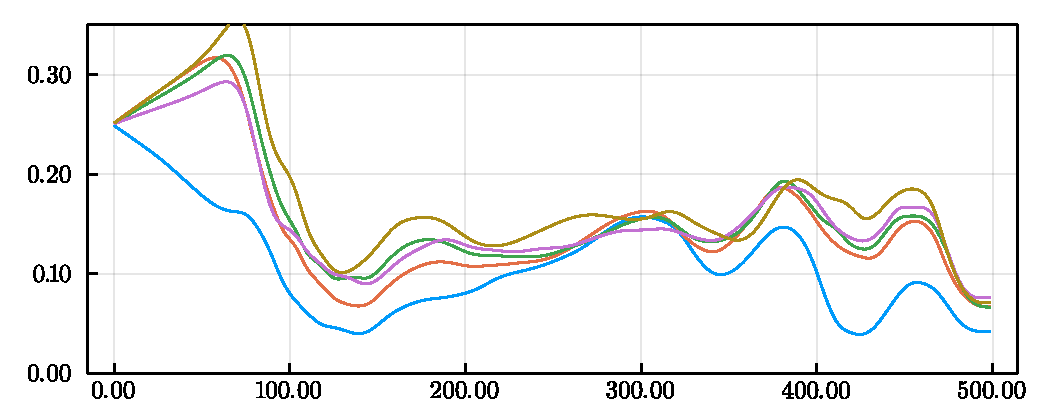
\includegraphics[width=\textwidth]{img/resultados/sensigammai_6-5_0alphaini0-15_0-1_0-45_high1__acov0-8_aini0-27675_gcov0-05gamma_e_0-1724_gamma_i_0-1389_beta_2_2-0000.pdf}
         \caption{\(1/\gamma_I = 6.5 [\text{días}]\)}
     \end{subfigure}
     \hfill
     \begin{subfigure}[b]{0.47\textwidth}
         \centering
         \includegraphics[width=\textwidth]{img/resultados/sensigammai_8-5_0alphaini0-15_0-1_0-45_high1__acov0-8_aini0-27675_gcov0-05gamma_e_0-1724_gamma_i_0-1389_beta_2_2-0000.pdf}
         \caption{\(1/\gamma_I = 8.5 [\text{días}]\)}
     \end{subfigure}
     \hfill
     \begin{subfigure}[b]{.47\textwidth}
         \centering
         \includegraphics[width=\textwidth]{img/resultados/sensigammai_10-5_0alphaini0-15_0-1_0-45_high1__acov0-8_aini0-27675_gcov0-05gamma_e_0-1724_gamma_i_0-1389_beta_2_2-0000.pdf}
         \caption{\(1/\gamma_I = 10.5 [\text{días}]\)}
     \end{subfigure}
     \hfill
     \begin{subfigure}[b]{.47\textwidth}
         \centering
         \includegraphics[width=\textwidth]{img/resultados/sensigammai_12-5_0alphaini0-15_0-1_0-45_high1__acov0-8_aini0-27675_gcov0-05gamma_e_0-1724_gamma_i_0-1389_beta_2_2-0000.pdf}
         \caption{\(1/\gamma_I = 12.5 [\text{días}]\)}
     \end{subfigure}
     \hfill
     \begin{subfigure}[b]{.47\textwidth}
         \centering
         \includegraphics[width=\textwidth]{img/resultados/sensigammai_14-5_0alphaini0-15_0-1_0-45_high1__acov0-8_aini0-27675_gcov0-05gamma_e_0-1724_gamma_i_0-1389_beta_2_2-0000.pdf}
         \caption{\(1/\gamma_I = 14.5 [\text{días}]\)}
     \end{subfigure}
     \hfill
    \caption[Sensibilidad factor sanitario estimado para los datos reales, ante distintos \(\gamma_I\).]{}
    \label{sensi-gammai-real}
\end{figure}




% Agrupar para usar datos reales, calcular Rt y comparar con Cori
\section{Evaluación del modelo mediante casos hipotéticos}\label{sec:evalmodel-casoshipot}

% Descripción de los tipos de cuarentena y las medidas de cuidado 
Las combinaciones entre los distintos niveles de cuidado y cuarentena presentados en \ref{met:evaluacion} dan lugar a una serie de casos, los cuales son presentados en la tabla \ref{table:casos-hipoteticos}. Se resuelve el sistema de ecuaciones diferenciales ordinarias \ref{eq:modelo-final} para cada caso, utilizando las distintas variantes de \(\alpha_i(t)\) y \(P(t)\), modificadas a partir de las estimaciones logradas en la sección anterior.

\begin{table}[h!]
\centering
\begin{tabular}{||l| c c c||} 
 \hline
 & \textbf{Cuidado insuficiente} & \begin{tabular}{@{}c@{}}\textbf{Cuidado} \\ \textbf{normal}\end{tabular} & \begin{tabular}{@{}c@{}}\textbf{Cuidado} \\ \textbf{extra}\end{tabular}\\ 
 \hline
 \textbf{Sin cuarentena} & Caso 1 & Caso 2 & Caso 3 \\ 
 \textbf{Cuarentena normal} & Caso 4 & Caso 5 & Caso 6 \\
 \textbf{Cuarentena fuerte} & Caso 7 & Caso 8 & Caso 9 \\
 \hline
\end{tabular}
\caption{Casos hipotéticos para distintas combinaciones de cuarentena y cuidado.}
\label{table:casos-hipoteticos}
\end{table}


Se prueban dos escenarios. En el primero de ellos, \(\beta_{\text{exterior}}\) es un valor mucho más grande que \(1\), de forma que la tasa de contagio está totalmente dominada por el ambiente exterior y prácticamente todos los contagios ocurren fuera de casa. Este se estudia en la subsección \ref{eval:beta-grande}. En el segundo, \(\beta_{\text{exterior}}\) es un valor mayor pero cercano a \(1\), de tal forma que el ambiente hogar contribuye a la tasa de contagios. Este se estudia en \ref{eval:beta-chico}.


\subsection{Escenario con contagio exterior predominante}\label{eval:beta-grande}


En este escenario se considera \(\beta_{\text{exterior}} >> 1\), de forma que la tasa de contagio está totalmente dominada por el ambiente exterior y las infecciones ocurren solamente en el exterior del hogar, las infecciones dentro del hogar son despreciables en comparación. Se utiliza \(\beta_{\text{exterior}} = 68.0\), pero los resultados son similares para un rango amplio de parámetros.

% Las figuras \ref{img:all-hip-S-N} y \ref{img:all-hip-I-N} presentan la evolución de los susceptibles \(S_i/N_i\) e infectados \(S_i/N_i\) (normalizados por el total de personas en cada clase), para cada uno de los casos. Se utilizan los mismos límites para los ejes \(y\) para facilitar la comparación.

Como era de esperarse, las diferencias socioeconómicas en la incidencia disminuyen debido a que la mayoría de los casos están utilizando, o bien la misma matriz de tiempos de residencia, o bien los mismos factores sanitarios, o incluso ambos.

La tabla \ref{table:descripcion-casos-hipot} describe los resultados para los distintos casos considerados, tomando como referencia el caso 5, de cuarentena y cuidado normal. En los casos 1 y 2, que corresponden a casos sin cuarentena con cuidado insuficiente o cuidado normal respectivamente, se contagia la gran mayoría de la población dentro de los primeros 6 meses considerados. En el caso con cuidado normal, la clase más acomodada resulta tener una incidencia bastante menor que las demás.

El cuidado extra logra contener la enfermedad con cuarentena normal o fuerte, como muestran los casos 6 y 9. La enfermedad desaparece rápidamente de entre la población en los primeros meses, aunque esto desde luego no considera importación de casos externos.

\begin{table}[H]
\centering
\begin{tabular}{||m{2.5cm}|m{4cm} m{4cm} m{4cm}||} 
 \hline
 & \begin{tabular}{@{}c@{}}\textbf{Cuidado} \\ \textbf{insuficiente}\end{tabular} & \begin{tabular}{@{}c@{}}\textbf{Cuidado} \\ \textbf{normal}\end{tabular} & \begin{tabular}{@{}c@{}}\textbf{Cuidado} \\ \textbf{extra}\end{tabular}\\ 
 \hline
 \textbf{Sin cuarentena} & \textit{Caso 1}: Se contagia un \(90\%\) de la población en los primeros 6 meses, de manera uniforme entre las distintas clases. Luego la enfermedad desaparece. & \textit{Caso 2}: Se contagia un \(65\%\) de la población de la clase alta en los primeros 6 meses, y un \(80\%\) de las demás clases. Luego la enfermedad desaparece. & \textit{Caso 3}: Se logra controlar el alza de casos, alcanzando el \textit{peak} de mediados de julio de 2020 y el de inicios de mayo de 2021 con menos de la mitad de casos, e incluso se evita el rebrote de junio de 2021. Ver figura \ref{img:esc-beta-grande-c3}.\\ 
 \textbf{Cuarentena normal} & \textit{Caso 4}: El primer \textit{peak} de julio de 2020 alcanza más del doble de casos y tiene una reducción lenta, de tal forma que el \textit{peak} de mayo de 2021 es apenas registrado como un alza ligera. Ver figura \ref{img:esc-beta-grande-c4}. & \textit{Caso 5}: Desarrollo real de la pandemia, tomado como referencia& \textit{Caso 6}: La enfermedad alcanza un pequeño \textit{peak} en julio de 2020 y luego se extingue.\\
 \textbf{Cuarentena fuerte} & \textit{Caso 7}: El primer \textit{peak} es muy similar en fecha y número de infectados, pero con un alza sostenida en el número de casos a partir septiembre de 2020, llegando a un \textit{peak} de más del doble de infectados en julio de 2021.  Ver figura \ref{img:esc-beta-grande-c7}. & \textit{Caso 8}: Se observan dos \textit{peaks} de unas 5000 personas, similar al Caso 3 pero sin poder contener el rebrote de junio de 2021. Ver figura \ref{img:esc-beta-grande-c8}. & \textit{Caso 9}: La enfermedad se extingue luego de los primeros meses. \\
 \hline
\end{tabular}
\caption{Observaciones para cada caso hipotético, escenario con \(\beta_{\text{exterior}} = 68\).}
\label{table:descripcion-casos-hipot}
\end{table}




% Aquí pongo todos los resultados de casos hipotéticos que obtuve... cuarentenas fuertes, etc... 
% \begin{figure}[h]
% \centering
% \includegraphics[width=0.99\textwidth]{img/resultados/allhipcases_S-N_commonylim0_1\parameterstring}
% \caption{Estimación de susceptibles, normalizados por el total de cada grupo \(S_i/N_i\), para cada caso hipotético.}
% \label{img:all-hip-S-N}
% \end{figure}

% \begin{figure}[h]
% \centering
% \includegraphics[width=0.99\textwidth]{img/resultados/allhipcases_I-N_commonylim0-015\parameterstring}
% \caption{Estimación de infectados normalizados por el total de cada grupo \(I_i/N_i\), para cada caso hipotético.}
% \label{img:all-hip-I-N}
% \end{figure}

La figura \ref{img:hip-3478-I-comp} muestra cuatro casos interesantes, comparándolos con la situación normal. En estos tres casos, el impacto es mayor sobre la clase 5 (prioridad alta, la más vulnerable). Esto puede atribuirse al hecho de que esa es la clase que presenta en general un mayor factor sanitario y movilidad, por lo que se verían más favorecidos si pudieran guardar las cuarentenas o las medidas de cuidado de mejor manera.
 
 El caso 3, que puede verse en \ref{img:esc-beta-grande-c3}, es interesante, ya que propone que la pandemia pudo controlarse incluso sin cuarentena, siempre y cuando todos pudieran evitar las aglomeraciones, usar mascarilla, lavado de manos y mantenerse lejos de los demás. El caso 4, en la figura \ref{img:esc-beta-grande-c4}, plantea que las medidas de higiene y cuidado sí fueron importantes, y que evitaron un \textit{peak} de más del doble de casos en los primeros meses de la pandemia. 
 
 
El caso 7, en la figura \ref{img:esc-beta-grande-c7}, afirma que una cuarentena más fuerte habría compensado una falta de preocupación o capacidad de cumplimiento de las medidas de higiene y cuidado, al menos en los primeros meses. La situación se desborda a medida que se acerca el 2021, debido a que la población sale del confinamiento. El caso 8, en la figura \ref{img:esc-beta-grande-c8}, es muy similar al caso 3, pero no logra evitar un segundo \textit{peak} en julio de 2021.

% Fechas 
% important_dates = [
%    Date(2020, 5, 13), # cuarentena total en la RM
%    Date(2020, 10, 25), # plesbicito por nueva constitución
%    Date(2021, 1, 4), # comienza a regir el permiso de vacaciones
%    Date(2021, 2, 1), # comienza un plan de vacunación más fuerte (según datos)
%    Date(2021, 5, 26) # un 50% de la población de Santiago tiene la primera dosis
%]
% casos interesantes: 3, 4, 7, 8

\begin{figure}[H]
     \centering
     \begin{subfigure}[b]{.47\textwidth}
         \centering
         \includegraphics[width=\textwidth]{img/resultados/comparecase_3withnormal_I_\parameterstring}
         \caption{Caso \(3\): Cuidado extra sin cuarentena.}
         \label{img:esc-beta-grande-c3}
     \end{subfigure}
     \hfill
     \begin{subfigure}[b]{.47\textwidth}
         \centering
         \includegraphics[width=\textwidth]{img/resultados/comparecase_4withnormal_I_\parameterstring}
         \caption{Caso \(4\): Cuidado insuficiente y cuarentena normal.}
         \label{img:esc-beta-grande-c4}
     \end{subfigure}
     \hfill
     \begin{subfigure}[b]{.47\textwidth}
         \centering
         \includegraphics[width=\textwidth]{img/resultados/comparecase_7withnormal_I_\parameterstring}
         \caption{Caso \(7\): Cuidado insuficiente y cuarentena fuerte.}
         \label{img:esc-beta-grande-c7}
     \end{subfigure}
     \hfill
     \begin{subfigure}[b]{.47\textwidth}
         \centering
         \includegraphics[width=\textwidth]{img/resultados/comparecase_8withnormal_I_\parameterstring}
         \caption{Caso \(8\): Cuidado normal y cuarentena fuerte.}
         \label{img:esc-beta-grande-c8}
     \end{subfigure}
     \hfill 
    \begin{subfigure}[b]{0.99\textwidth}
    \centering
    \scalebox{0.7}{
    \begin{tikzpicture}
	\begin{pgfonlayer}{nodelayer}
		\node [style=none] (50) at (5, 0) {};
		\node [style=none] (51) at (7, 0) {};
		\node [style=none] (52) at (6, -0.5) {Prioridad Alta};
		\node [style=none] (53) at (2, 0) {};
		\node [style=none] (54) at (4, 0) {};
		\node [style=none] (55) at (3, -0.5) {Prioridad};
		\node [style=none] (56) at (-1, 0) {};
		\node [style=none] (57) at (1, 0) {};
		\node [style=none] (58) at (0, -0.5) {Prioridad};
		\node [style=none] (59) at (-4, 0) {};
		\node [style=none] (60) at (-2, 0) {};
		\node [style=none] (61) at (-3, -0.5) {Prioridad Baja};
		\node [style=none] (62) at (-7, 0) {};
		\node [style=none] (63) at (-5, 0) {};
		\node [style=none] (64) at (-6, -0.5) {Sin Prioridad};
		\node [style=none] (65) at (0, -1) {Media Baja};
		\node [style=none] (66) at (3, -1) {Media Alta};
	\end{pgfonlayer}
	\begin{pgfonlayer}{edgelayer}
		\draw [style=class5] (50.center) to (51.center);
		\draw [style=class1] (62.center) to (63.center);
		\draw [style=class2] (59.center) to (60.center);
		\draw [style=class3] (56.center) to (57.center);
		\draw [style=class4] (53.center) to (54.center);
	\end{pgfonlayer}
\end{tikzpicture}

    }
    \end{subfigure}
        \caption[Personas infectadas para casos hipotéticos seleccionados. Escenario \(\beta_{\text{exterior}} >> 1\).]{Personas infectadas para caso hipotéticos seleccionados, con la estimación de los casos reales de fondo. Diferentes límites para el eje \(y\). Las líneas grises corresponden a las fechas relevantes de la tabla \ref{table:fechas-relevantes}.}
        \label{img:hip-3478-I-comp}
\end{figure}


\subsection{Escenario con contagio en hogar}\label{eval:beta-chico}


En este caso se buscó un valor donde existiera contagio en el hogar, y se eligió \(\beta_{\text{exterior}} = 1.2\). Esto se hizo estudiando las contribuciones de los ambientes a la tasa de contagio, calculando las contribuciones a la derivada de cada ambiente dadas por \ref{eq:contribuciones-j}, en la subsección \ref{met-subsec:fijos}. Bajo estas condiciones, se observa que la cuarentena prácticamente no influye en el número de contagios; lo que realmente determina si se controla o no la pandemia es el factor sanitario. Los resultados se sintetizan en la tabla \ref{table:descripcion-casos-hipot-beta-1-2}, y los casos de interés elegidos anteriormente se presentan en la figura \ref{img:hip-3478-I-comp-beta1-2}.



\begin{table}[h!]
\centering
\begin{tabular}{||m{2.5cm}|m{4cm} m{4cm} m{4cm}||} 
 \hline
 & \begin{tabular}{@{}c@{}}\textbf{Cuidado} \\ \textbf{insuficiente}\end{tabular}  & \begin{tabular}{@{}c@{}}\textbf{Cuidado} \\ \textbf{normal}\end{tabular} & \begin{tabular}{@{}c@{}}\textbf{Cuidado} \\ \textbf{extra}\end{tabular}\\ 
 \hline
 \textbf{Con o sin cuarentena} & \textit{Casos 1, 4 y 7}: Se observan \textit{peaks} de más del doble de casos que el normal, y que se reducen más lentamente. El número de contagios no baja del \(0.5\%\) de la población. Ver figuras \ref{img:esc-beta-chico-c4} y \ref{img:esc-beta-chico-c7}. & \textit{Caso 2, 5 y 8} Muy similares al caso 5, el normal usado como referencia. Ver figura \ref{img:esc-beta-chico-c8}. & \textit{Caso 3, 6, y 9}: La enfermedad tiene un pequeño \textit{peak} en torno a julio de 2020 y se extingue luego de unos meses. Ver figura \ref{img:esc-beta-chico-c3}. \\
 \hline
\end{tabular}
\caption[Observaciones para cada caso hipotético, escenario con \(\beta_{\text{exterior}} = 1.2\)]{Observaciones para cada caso hipotético, escenario con \(\beta_{\text{exterior}} = 1.2\). Tabla condensada, puesto que no hay variaciones importantes con respecto a la fuerza de la cuarentena.}
\label{table:descripcion-casos-hipot-beta-1-2}
\end{table}



\begin{figure}
     \centering
     \begin{subfigure}[b]{.47\textwidth}
         \centering
         \includegraphics[width=\textwidth]{img/resultados/comparecase_3withnormal_I_gamma_e_0-1724_gamma_i_0-0833_beta_2_2-0000.pdf}
         \caption{Caso \(3\): Cuidado extra sin cuarentena.}
         \label{img:esc-beta-chico-c3}
     \end{subfigure}
     \hfill
     \begin{subfigure}[b]{.47\textwidth}
         \centering
         \includegraphics[width=\textwidth]{img/resultados/comparecase_4withnormal_I_gamma_e_0-1724_gamma_i_0-0833_beta_2_2-0000.pdf}
         \caption{Caso \(4\): Cuidado insuficiente y cuarentena normal.}
         \label{img:esc-beta-chico-c4}
     \end{subfigure}
     \hfill
     \begin{subfigure}[b]{.47\textwidth}
         \centering
         \includegraphics[width=\textwidth]{img/resultados/comparecase_7withnormal_I_gamma_e_0-1724_gamma_i_0-0833_beta_2_2-0000.pdf}
         \caption{Caso \(7\): Cuidado insuficiente y cuarentena fuerte.}
         \label{img:esc-beta-chico-c7}
     \end{subfigure}
     \hfill
     \begin{subfigure}[b]{.47\textwidth}
         \centering
         \includegraphics[width=\textwidth]{img/resultados/comparecase_8withnormal_I_gamma_e_0-1724_gamma_i_0-0833_beta_2_2-0000.pdf}
         \caption{Caso \(8\): Cuidado normal y cuarentena fuerte.}
         \label{img:esc-beta-chico-c8}
     \end{subfigure}
     \hfill
    \begin{subfigure}[b]{0.99\textwidth}
    \centering
    \scalebox{0.6}{
    \begin{tikzpicture}
	\begin{pgfonlayer}{nodelayer}
		\node [style=none] (50) at (5, 0) {};
		\node [style=none] (51) at (7, 0) {};
		\node [style=none] (52) at (6, -0.5) {Prioridad Alta};
		\node [style=none] (53) at (2, 0) {};
		\node [style=none] (54) at (4, 0) {};
		\node [style=none] (55) at (3, -0.5) {Prioridad};
		\node [style=none] (56) at (-1, 0) {};
		\node [style=none] (57) at (1, 0) {};
		\node [style=none] (58) at (0, -0.5) {Prioridad};
		\node [style=none] (59) at (-4, 0) {};
		\node [style=none] (60) at (-2, 0) {};
		\node [style=none] (61) at (-3, -0.5) {Prioridad Baja};
		\node [style=none] (62) at (-7, 0) {};
		\node [style=none] (63) at (-5, 0) {};
		\node [style=none] (64) at (-6, -0.5) {Sin Prioridad};
		\node [style=none] (65) at (0, -1) {Media Baja};
		\node [style=none] (66) at (3, -1) {Media Alta};
	\end{pgfonlayer}
	\begin{pgfonlayer}{edgelayer}
		\draw [style=class5] (50.center) to (51.center);
		\draw [style=class1] (62.center) to (63.center);
		\draw [style=class2] (59.center) to (60.center);
		\draw [style=class3] (56.center) to (57.center);
		\draw [style=class4] (53.center) to (54.center);
	\end{pgfonlayer}
\end{tikzpicture}

    }
    \end{subfigure}
        \caption[Personas infectadas para caso hipotéticos seleccionados.]{Personas infectadas para caso hipotéticos seleccionados, con la estimación de los casos reales de fondo. Diferentes límites para el eje \(y\). Las líneas grises corresponden a las fechas relevantes de la tabla \ref{table:fechas-relevantes}.}
        \label{img:hip-3478-I-comp-beta1-2}
\end{figure}


% Esto ya es solo una pregunta... pero se puede hacer el proceso a la inversar? obtener estimaciones de movilidad para distintos grupos usando los datos de infecciones.... el problema es que el mejor indicador son los fallecidooooos y los resultados dependen mucho de las tasas de muerte.

\chapter{Discusión} \label{chap:discus}

A continuación se ofrece una discusión con respecto al trabajo realizado. La sección \ref{dis:caso} comenta los resultados obtenidos para el caso de estudio y para las situaciones hipotéticas, resaltando las limitaciones derivadas de los supuestos y simplificaciones hechos a lo largo del modelamiento, y presentando posible interpretaciones. La sección \ref{dis:metod} comenta la metodología seguida, presenta algunos enfoques alternativos con que se podría haber abordado el trabajo, expone posibles extensiones y discute el cumplimiento de los objetivos.

\section{Acerca del caso de estudio}\label{dis:caso}

En primer lugar, es necesario recordar los supuestos y simplificaciones hechos a la hora de modelar el caso de estudio. Por un lado, se consideró que la población en la Región Metropolitana se mantenía constante, despreciando efectos como la natalidad, mortalidad debido a causas naturales y efectos migratorios entre ciudades. Por otro lado, algunos factores relevantes a la transmisión del COVID-19 fueron dejados fuera al utilizar un modelo SEIR, como la existencia de casos sin síntomas o con síntomas leves, que pueden o no ser reportados y que también transmiten el virus \cite{Li2020c}\cite{Byambasuren2020}\cite{Gao2021}. El supuesto de que todas las clases socioeconómicas tienen la misma tasa de incubación y recuperación es un factor que debe ser considerado, especialmente al tener en cuenta el estudio de sensibilidad presentado en \ref{subsec:sensigamma}.

La movilidad... los casos no reportados

El uso del filtro de Kalman tiene, desde luego, limitaciones; teóricamente solo puede justificarse en el caso lineal, y el uso del filtro extendido lleva a errores numéricos que podrían mitigarse usando un filtro más apto para tratar con no linealidades, como el filtro \textit{unscented}. El estudio del caso sintético muestra también que el filtro tiene dificultades para estimar los valores sanitarios al comienzo de la pandemia, cuando hay muy pocos casos, por lo que los resultados en la fase inicial son poco confiables. Los estudios de sensibilidad mostraron además las diferencias en las estimaciones, dependiendo de los valores de varianzas elegidas como parámetros del filtro.

El número de casos detectados no es la mejor observación; se ha hablado de cómo la capacidad de detectar los nuevos contagios difiere entre clases socioeconómicas \cite{Mena2021}, sugiriendo que el número de fallecidos es una mejor medida. Esto sin embargo, sugiere que el número de casos está subestimado para las clases más vulnerables, lo que solo contribuye a resaltar los resultados obtenidos.

Una medida de gran relevancia que no fue considerada en el modelo fue la vacunación. Esta, sin embargo, debería verse directamente reflejada en una disminución importante del factor sanitario una vez que se vacuna gran parte de la población.

%%% Factor sanitario 
Con respecto a los resultados obtenidos, se destaca el hecho de que el factor sanitario de la clase más acomodada se mantiene por debajo de las demás clases. Ese resultado es constante a través de los análisis de sensibilidad. Se intentó inicialmente obtener un factor sanitario común a todas las clases, lo que sugeriría que todos enfrentan el mismo riesgo en el exterior, pero no fue posible obtener resultados razonables.

Todo esto sugiere que las diferencias en movilidad por sí solas no son suficientes para explicar las diferencias en la cantidad de contagios. Las clases socioeconómicas más vulnerables no solo no pueden guardar las cuarentenas de la misma forma que las clases acomodadas, sino que además, al salir al exterior, se encuentran en ambientes más riesgosos, ya sea por estar en ambientes más concurridos, o por no utilizar adecuadamente las medidas de seguridad como el lavado de manos y el uso correcto de mascarillas. Estos resultados son consistentes con los encontrados por \cite{Chang2021}. Otras posibles explicaciones podrían ser las diferencias en la capacidad de testeo y trazabilidad \cite{Bennett2021}\cite{Mena2021}.

Con respecto al ajuste del factor sanitario, a pesar de la gran incerteza que surge de utilizar valores grandes de covarianza, el caso sintético sugiere que se obtienen mejores resultados de esta forma. Los resultados deben considerar además los estudios de sensibilidad de la subsección \ref{subsec:sensigamma}. Mientras la hipótesis \(\gamma_{Ei} = \gamma_E\) y \(\gamma_{Ii} = \gamma_I\) sea válida, es decir, que las tasas de incubación y remoción son iguales en cada clase, se puede esperar que las estimaciones del factor sanitario \(\alpha_i\) se expandan o contraigan uniformemente. La tasa de exposición \(\gamma_E\) no tiene gran relevancia, sin embargo, la de recuperación \(\gamma_I\) puede hacer variar considerablemente los resultados. Ahora bien, para subestimar el factor sanitario, se debería tener un tiempo de recuperación mayor, pero esto es improbable considerando que el acceso a salud es superior en las clases más acomodadas.

Destaca el factor sanitario en el periodo mayo-junio de 2021, donde se observa que la clase más acomodada consigue una reducción mucho más marcada que las demás. Una posible hipótesis sería atribuir esto al avance del proceso de vacunación en Chile, que para esas fechas ya había superado el 50\% de población vacunada en la Región Metropolitana (ver figura \ref{img:cmm-vacunados}); ¿fue el proceso de vacunación más marcado en las comunas acomodadas? La distribución de vacunas ocurrió por tramos de edad, de mayores a jóvenes, y la distribución de adultos mayores en las comunas acomodadas es mayor.

%% Casos hipotéticos 
Con respecto a los casos hipotéticos, se observan dos escenarios que dependen del valor del riesgo \(\beta_{\text{exterior}}\). Para este análisis ese necesario considerar el aporte a la derivada de cada uno de los ambientes, calculado en \ref{}. 
Por un lado, al usar un valor notoriamente mayor que \(1\) (\(\beta_{\text{exterior}} = 10\), el aporte a la derivada dado por el ambiente \(\text{hogar}\) es despreciable en comparación al dado por el \(\text{exterior}\). Esto quiere decir que prácticamente todos los contagios ocurren cuando la gente sale de su hogar. Esto, sin embargo, no es consistente con \cite{Ferguson2020}, quien afirma que aproximadamente 1/3 de los contagios ocurren en el hogar. Incluso en esta situación, se observa que las medidas de cuidado son sumamente relevantes, pudiendo prevenir un segundo \textit{peak} como muestra el caso 3.

Por otro lado, cuando se usa un valor ligeramente mayor a \(1\) (\(\beta_{\text{exterior}} = 1.2\) por ejemplo) el aporte del ambiente \texttt{hogar} a la derivada ya es perceptible \texttt{exterior} (para este caso en particular, es unas 10 veces menor). El estudio de los casos hipotéticos, sin embargo, revela que la cuarentena casi no influya en nada en los resultados finales, y que todo depende de las medidas de cuidado.

El modelo en ambos escenarios coincide, sin embargo, en que si fuera posible que todos se cuidaran al mismo nivel que el grupo más acomodado, se podría controlar el virus incluso sin la exigencia de cuarentenas.

\section{Acerca de la metodología}\label{dis:metod}

  

% Cómo influyeron las decisiones tomadas en los resultados? 

% Matriz de tiempos de residencia - EOD2012

Una de las diferencias distintivas de este enfoque es utilizar los datos de movilidad para estimar tiempos de residencia, siguiendo la forma lagrangiana. Esta no era la única forma posible, los datos de la Encuesta Origen Destino contienen información detallada de viajes, incluyendo comunas de salida y llegada. Usando esto, una forma alternativa de usar la Encuesta habría sido usar sus datos como movilidad basa entre las distintas comunas, y aprovechar los datos de movilidad en pandemia, como los del ISCI presentados en la sección \ref{}, para modificar estos viajes, siguiendo una metodología similar a \cite{Lai2020}.


De seguir esta forma de trabajo, habría sido posible definir algo análogo al factor sanitario, para cada comuna. El no tener una distinción entre clases y ambientes sin embargo, impone el tener que trabajar únicamente con divisiones espaciales, como zonas censales, comunas y agrupaciones de comunas, dificultando el trabajo con grupos etarios.

Ahora, si bien la metodología propuesta sí permite sortear esta dificultad, no se elimina completamente, puesto que sigue siendo necesario estimar los tiempos de residencia para cada una de las clases, y la forma en que estos variaron en cada ambiente no fue uniforme en distintos grupos etarios. A modo de ejemplo, podría ser posible considerar grupos etarios, puesto que existen series de tiempo de número de contagios agrupados por edad. La variación de movilidad por grupo etario, sin embargo, no es tan fácil de obtener, considerando que hay grupos mal representados en los datos disponibles; los datos de ISCI por ejemplo, se derivan del uso de torres de telefonía móvil, que en el caso de niños y adultos mayores podría no ser adecuado.

Al intentar agregar más ambientes al análisis, surgen problemas similares. Los datos más cercanos a movilidad por ambiente en pandemia son los provistos por Google, presentados en la sección \ref{}. Estos datos están agrupados a nivel regional/provincial, pero se sabe \cite{Olivares2020} que no son uniformes entre distintos niveles socioeconómicos; el teletrabajo es mucho más común en niveles altos, mientras que un porcentaje importante de la población más vulnerable tiene trabajos esenciales que no pueden detenerse en pandemia \cite{}.

Debido a este problema, la Encuesta Origen Destino terminó jugando un rol muy secundario en el trabajo, ya que su utilidad se vio relegada a una simple estimación del tiempo que pasaban en el hogar, antes de la pandemia, los distintos grupos socioeconómicos, y habría sido de mejor aprovechada siguiendo la metodología euleriana antes propuesta. 

La metodología propuesta, sin embargo, presenta la ventaja de ser utilizable con menos datos de movilidad disponible, por lo que a aplicable incluso en regiones donde no se tenga el detalle de las tasas de movilidad entre cada par de zonas; solo es necesario saber cuánto se mueve la gente, no hacia dónde lo hace, debido a que todos interactúan en un ambiente \texttt{exterior} común.

Una desventaja no prevista en un principio es la estimación de los riesgos específicos por ambiente; no es tan clara como se supuso. Esto quedó en evidencia al observar los resultados de la sección \ref{sec:evalmodel-casoshipot}. Estimaciones de la forma: ``aproximadamente 1/3 de los contagios ocurren en el hogar'' \cite{Ferguson2020} no se traducen directamente en asignar \( 2 \beta_{\text{hogar}} = \beta_{\text{exterior}}\).

% Conclusión del análisis de sensibilidad

El framework propuesto puede aplicarse a una amplia variedad de modelos, compartimientos, parámetros y observaciones. Algunas posibles extensiones son considerar los efectos de la vacunación en los compartimientos, usar comunas en lugar de grupos socioeconómicos, usar un filtro que se comporte mejor frente a no linealidades (como el filtro \textit{unscented} o ``sin olor''), ampliar el modelo para considerar fallecidos, etc.

Un aporte lateral del trabajo realizado es el código realizado, que se encuentra disponible en línea en la plataforma GitHub. El repositorio \url{} contiene una implementación en Matlab del algoritmo de extracción de tiempos de residencia mencionado brevemente en \cite{Munizaga2011}. El repositorio \url{} tiene la librería KalmanFilter.jl, documentada, modular y extensible, desarrollada en el lenguaje Julia, que permite trabajar con Filtro de Kalman lineal, extendido y ``sin olor`` en sus versiones continuas y discretas, utilizando observadores lineales y no lineales. Finalmente, el repositorio \url{} contiene el código utilizado en el análisis del caso de estudio del COVID-19 en Santiago. Este repositorio hace uso de la novedosa librería ModelingToolkit.jl \cite{}, aun en una fase inicial de desarrollo, la cual, de forma similar a Modellica o ... [insertar software] ofrece herramientas para el trabajo con modelos de ecuaciones diferenciales, cálculo simbólico de derivadas, de forma eficiente, y extensible.

% Comparación con la literatura de la metodología 
% Se cumplieron los objetivos?? Era atingentes los objetivos? 

Los objetivos específicos fueron logrados en su mayor parte, puesto que fue posible plantear una forma de estimar el factor sanitario y realizar una implementación para el caso de estudio. Sin embargo, era deseable poder incluir en el modelo ambientes como \texttt{trabajo}, \texttt{estudios}, \texttt{compras} o \texttt{transporte público}, o considerar grupos etarios, y esto no fue logrado.
\chapter{Conclusiones}

%\nocite{*} % esto hace que se vean todas
\bibliographystyle{ieeetr}
\bibliography{library}

\appendix

\chapter{Sistemas lineales y no lineales, continuos y discretos} \label{sec:lineal}

Si bien la mayoría de los modelos en la vida real son no lineales --los modelos epidemiológicos en particular-- las herramientas disponibles para estimación y control están mucho más entendidas y son más accesibles en los sistemas lineales. [parafrasis del Simon]


\section{Sistemas lineales continuos}

En esta sección se incluye un recordatorio de la teoría de sistemas lineales. 

Un sistema lineal determinista a tiempo continuo es de la forma 

\[
\begin{aligned}
x'(t) &= Ax(t) + Bu(t) \\
y(t) &= Cx(t)
\end{aligned}
\]

donde \(x\) es el vector de estados, \(u\) un vector control e \(y\) es un vector de salida. \(A, B, C\) son matrices de dimensiones adecuadas. \(A\) es llamada matriz del sistema, \(B\) es la matriz de \textit{input} y \(C\) la matriz de \textit{output}.\\





\section{Sistemas no lineales continuos}


En la mayoría de aplicaciones, sin embargo, se trabaja con sistemas no lineales. Un sistema no lineal a tiempo continuo es de la forma 

\[
\begin{aligned}
x' = f(x,u,w) \\
y = h(x,v)
\end{aligned}
\]

donde \(f(\cdot), h(\cdot)\) son funciones arbitrarias que devuelven vectores. \(w\) se usa para indicar ruido del proceso y \(v\) para el ruido en las mediciones. Si dependen explícitamente de \(t\), entonces el sistema es variable en el tiempo; si no, es tiempo invariante. 

La aproximación lineal de un sistema no lineal en torno a un punto \( (\bar{x}, \bar{u}, \bar{w})\) es 

\[
\begin{aligned}
x'  &= f(x,u,w) \\
    & \approx f(\bar{x}, \bar{u}, \bar{w}) + \left.\frac{\partial f}{\partial x} \right|_{\bar{x}}(x-\bar{x}) +
    \left.\frac{\partial f}{\partial u} \right|_{\bar{u}}(u-\bar{u}) + 
    \left.\frac{\partial f}{\partial w} \right|_{\bar{w}}(w-\bar{w}) \\
    &= \bar{x}' + A\tilde{x} + B\tilde{u} + L\tilde{w}
\end{aligned}
\]
Lo que nos permite escribir un sistema lineal para \(\tilde{x} = x - \bar{x}\)
\[
\tilde{x}' = A\tilde{x} + B \tilde{u} + L \tilde{w}
\]
Como \(w\) es ruido, podemos tomar \(\bar{w}=0\), lo que nos deja 
\[
\tilde{x}' = A\tilde{x} + B \tilde{u} + L w
\]

Similarmente, se puede obtener una versión linealizada de la ecuación de mediciones.

\[
\begin{aligned}
\tilde{y} &= \left. \frac{\partial f}{\partial x} \right|_{\bar{x}} \tilde{x} + \left. \frac{\partial f}{\partial v} \right|_{\bar{v}} \tilde{v}
\end{aligned}
\]


\section{Sistemas discretos y esquemas de discretización}

En la práctica, al trabajar en un computador solo contamos con sistemas discretos, ya sean lineales

\[
x_{n+1} = F_n x_n
\]

o no lineales 
\[
x_{n+1} = f(x_n, t_n)
\]

Una técnica importante, por tanto, será la de discretizar sistemas continuos. Una ecuación diferencial de la forma 
\[
x' = f(x,u,w) 
\]
can be rewritten as 
\[
x(t) = x(t_0) + \int_{t_0}^{t} f(x(s), s) ds
\]
Dividiendo el intervalo \([t_0, t]\) con una grilla de puntos \(t_0 < t_1 < \dots < t_N < t\), obtenemos la siguiente recursión 

\[
\begin{aligned}
x(t_{n+1}) &= x(t_n) + \int_{t_n}^{t_{n+1}} f(x(s), s) ds
\end{aligned}
\]
Lo que reduce el problema a encontrar una aproximación para la integral de la derecha. 

La forma más sencilla de hacer esto es con la \textbf{integración rectangular}. Supone que, si el intervalo \([t_n, t_{n+1}]\) es pequeño, entonces \(f\) varía poco y puede ser aproximada por \(f(x(t_n), t_n)\). Si suponemos además que la grilla es equiespaciada, ie \( t_{n+1}-t_n = \Delta t \) para cada \(n\), entonces el método de \textbf{Euler explícito} entrega la aproximación: 
\[
x(t_{n+1}) = x(t_n) + \Delta t f(x(t_{n}), t_n)
\]

Un supuesto similar, que \(f\) es constante en todo el intervalo, pero aproximando por \(f(x(t_{n+1}), u(t_{n+1}), t_{n+1})\) da lugar al un método de \textbf{Euler implícito}, que requiere 

\[
x(t_{n+1}) = x(t_n) + \Delta t f(x(t_{n+1}), t_{n+1})
\]

Un método explícito ampliamente conocido es el de \textbf{Runge-Kutta de orden 4}, que hace más evaluaciones de la función en cada paso para obtener mayor precisión. 

\begin{equation}\label{eq:rk4}
\begin{aligned}
t_{n + 1/2} &:= t_n + \Delta t / 2\\
\Delta x_1 &= f(x(t_n), t_n) \\
\Delta x_2 &= \Delta t f(x(t_n) + \Delta x_1, t_{n + 1/2}) \\
\Delta x_3 &= \Delta t f(x(t_n) + \Delta x_2, t_{n + 1/2}) \\
\Delta x_4 &= \Delta t f(x(t_n) + \Delta x_3, t_{n + 1}) \\
\end{aligned}
\end{equation}
para hacer la estimación final 
\[
x(t_{n+1}) = x(t_n) + \frac{1}{6}\Big( \Delta x_1  +  2\Delta x_2 + 2\Delta x_3 +\Delta x_4\Big)
\]

\section{Observabilidad} 

Hay un último concepto que nos será de utilidad.

\begin{defn}[Observabilidad]
Un sistema a tiempo continuo es observable si para cualquier estado inicial \(x(0)\) y cualquier tiempo final \(t > 0\) el estado inicial \(x(0)\) puede ser determinado únicamente conociendo el \textit{input} \(u(\tau)\) y el \textit{output} \(y(\tau)\) para \(\tau \in [0,t]\).
\end{defn}

\begin{teo}
El sistema lineal a tiempo continuo invariante de \(n\) estado 
\[
\begin{aligned}
x' &= Ax + Bu \\
y' &= Cx
\end{aligned}
\]
tiene la matriz de observabilidad 
\[
Q = \begin{pmatrix}
C \\
CA \\
\vdots \\
CA^{n-1}
\end{pmatrix}
\]
El sistema es observable si y solo si \(\text{rank}(Q) = n\).\\
\end{teo}


\end{document}
